\chapter{การออกแบบระบบและรายละเอียดการพัฒนา}
\label{chapter:experiment}

\section{ภาพรวมของเว็บแอพพลิเคชั่น}

เว็บแอพพลิเคชั่นประเมินความสามารถเบื้องต้นของผู้สมัครงาน คือระบบที่จะช่วยให้คัดกรองผู้คนได้มีประสิทธิภาพมากยื่งขึ้น ผ่านการทำข้อสอบที่สามารถกำหนดระดับความยากของข้อสอบได้ และดึงคลังคำถามมาแบบสุ่ม เพื่อส่งให้ผู้สมัครงานโดยอัติโนมัติผ่านทางอีเมล เมื่อผู้สมัครงานทำข้อสอบเสร็จแล้ว ข้อสอบจะถูกส่งไปที่ผู้ออก พร้อมตรวจข้อที่เป็นคำถามปรนัยให้อัตโนมัติ โดยระบบนี้แบ่งเป็น 2 ส่วนหลักๆ คือส่วนต่อประสานกับผู้ใช้ที่พัฒนาด้วย Vue.js framwork และส่วนที่จัดการกับฐานข้อมูล พัฒนาด้วย Node.js framwork โดยการเก็บข้อมูลทั่วไปถูกเก็บอยู่ใน mongoDB และการเก็บไฟล์ เช่น ไฟล์รูปภาพ จะถูกเก็บอยู่บน Google Cloud Storage การจัดการอีเมลใช้บริการของ SendGrid เข้ามาช่วยจัดการซึ่งสามารถวิเคราะห์การส่งอีเมลในแต่ละครั้งได้ และการยืนยันตัวตนจะถูกเข้ารหัสด้วย JOSN Web Token ภาพรวมการทำงานของระบบจะเป็นดังรูป 3.1

\begin{figure}[H]
  \centering
  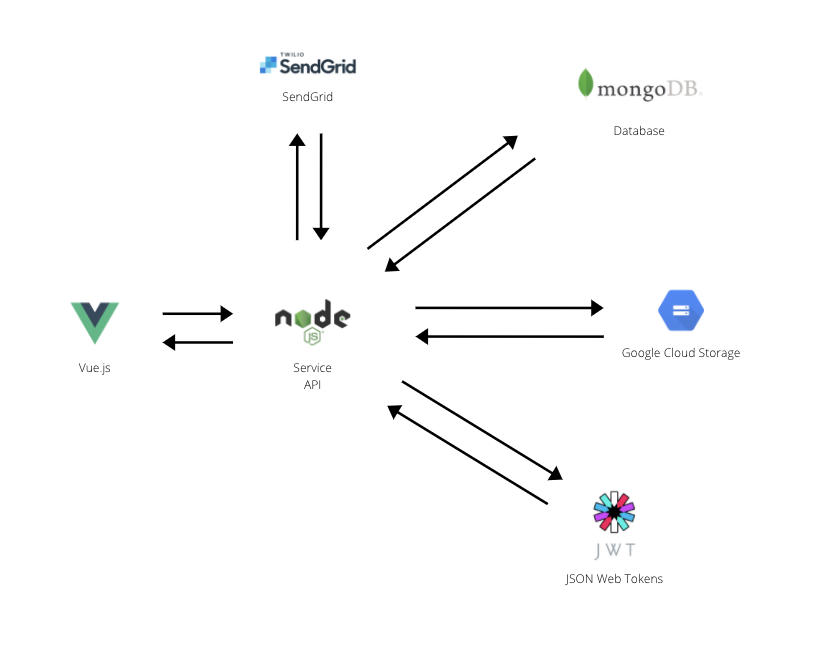
\includegraphics[width=0.9\columnwidth]{ExamaSystem.png}
  \caption{แสดงการทำงานขอเว็ปแอพพลิเคชั่นประเมินความสามารถเบื้องต้นของผู้สมัครงาน}
  \label{Fig:ExamaSystem}
\end{figure}

\newpage
\section{วิเคราะห์ความต้องการ}

\subsection{ความต้องการที่เป็นหน้าที่หลักของระบบ (Functional Requirement)}
\begin{enumerate}
  \item ผู้ใช้งานสามารถสามารถลงทะเบียนเป็นสมาชิกเพื่อใช้งานเว็บแอพพลิเคชั่นได้   
  \item ผู้ใช้ต้องยืนยันตัวตนผ่านอีเมลหลังจากทำการลงทะเบียน ถึงจะเข้าใช้งานระบบได้
  \item ผู้ใช้งานสามารถสร้าง, แก้ไข และลบคำถามในหมวดหมู่คำถามได้
  \item ระบบสามารถป้องกันการรีเฟรชเพจ หรือการเปลี่ยนหน้าได้ หากผู้ใช้กำลังสร้างหรือแก้ไขคำถามในหมวดหมู่คำถาม
  \item ผู้ใช้งานสามารถยกเลิกการสร้างหมวดหมู่คำถามได้
  \item ผู้ใช้งานไม่สามารถลบหมวดหมู่คำถามได้ หากหมวดหมู่นั้นถูกใช้งานอยู่ในข้อสอบ
  \item ผู้ใช้งานสามารถสร้างคำถามประเภท ปรนัย, อัตนัย และคำถามที่มีไฟล์แนบได้
  \item คำถามที่เป็นปรนัย สามารถเลือกให้มีข้อถูกมากกว่า 1 ข้อได้
  \item สามารถใส่รูปภาพเพิ่มในตัวเลือกคำตอบของคำถามประเภทปรนัยได้
  \item หากผู้ใช้งานส่งข้อสอบให้ผู้สมัครงานทำแล้ว ถ้าหมวดหมู่คำถามนั้นถูกใช้งานในข้อสอบ คำถามในหมวดหมู่นั้นจะสามารถแก้ไขได้เฉพาะเฉลยเท่านั้น ไม่สามารถแข้ไขคำถามได้ โดยหากต้องการแก้ไขให้ทำการคัดลอกหมวดหมู่คำถามของตนเองมาแก้ไขเป็นหมวดหมู่ใหม่
  \item ผู้ใช้งานสามารถคัดลอกหมวดหมู่คำถามของตนเองได้
  \item ผู้ใช้งานสามารถเปิดหมวดหมู่คำถามให้เป็นสาธารณะได้
  \item หมวดหมู่คำถามที่เป็นสาธารณะ ผู้ที่ไม่ใช้เจ้าของไม่สามารถแก้ไขได้ โดยผู้ใช้สามารถคัดลอกหมวดหมู่คำถามที่เป็นสาธารณะไปเป็นเป็นของตนเองได้ หากผู้ใช้ไม่ใช้เจ้าของแต่ต้องการแก้ไข
  \item ผู้ใช้งานสามารถค้นหาหมวดหมู่คำถามได้
  \item ผู้ใช้งานสามารถสร้างข้อสอบ ที่กำหนดหมวดหมู่คำถามที่ต้องการ,จำนวนข้อ และความยากได้ โดยข้อสอบจะทำการสุ่มเมื่อผู้ใช้ส่งให้ผู้ทำข้อสอบ
  \item ระบบสามารถป้องกันการรีเฟรชเพจ หรือการเปลี่ยนหน้าได้ หากผู้ใช้กำลังสร้างหรือแก้ไขข้อสอบ
  \item ผู้ใช้สามารถลบแก้ไขหมวดหมู่คำถามที่ใช้, จำนวนข้อ และระดับความยากของข้อสอบได้
  \item ผู้ใช้สามารถค้นหาข้อสอบได้
  \item ผู้ใช้สามารถเปิดข้อสอบให้เป็นสาธารณะได้
  \item ข้อสอบที่เป็นสาธารณะ ผู้ที่ไม่ใช้เจ้าของไม่สามารถแก้ไขได้ โดยผู้ใช้สามารถคัดลอกข้อสอบสาธารณะไปเป็นเป็นของตนเองได้ หากผู้ใช้ไม่ใช้เจ้าของแต่ต้องการแก้ไข
  \item หากผู้ใช้งานส่งข้อสอบให้ผู้สมัครงานทำแล้ว ข้อสอบที่ผู้ใช้งานสร้างขึ้นนั้นจะไม่สามารถแก้ไขได้ แต่สามารถส่งให้ผู้สมัครงานคนอื่นทำต่อไปได้ โดยระบบจะทำการสุ่มคำถามที่ผู้ออกข้อสอบกำหนด จำนวนข้อประเภทคำถาม และระดับความยาก
  \item ผู้ใช้งานสามารถดูประวัติที่ผู้ใช้ทำการส่งข้อสอบให้ผู้สมัครงานได้
  \item ผู้ใช้สามารถกำหนดระยะเวลาการทำข้อสอบได้
  \item ผู้ใช้สามารถกำหนดวันหมดอายุของข้อสอบได้
  \item ผู้ใช้สามารถส่งข้อสอบให้ผู้สมัครงานผ่านอีเมลได้
  \item ผู้ทำข้อสอบสามารถเข้ามาทำข้อสอบในเว็บแอพพลิเคชั่นได้ตลอด หากเวลาในการทำข้อสอบยังไม่หมด
  \item เมื่อผู้ทำข้อสอบทำการส่งข้อสอบแล้ว ระบบสามารถตรวจข้อสอบที่เป็นปรนัยได้
  \item มีการแสดงสถานะบอกว่าผู้ใช้งาน ตรวจข้อสอบนั้นหรือยัง
  \item มีการสรุปคะแนนรวมของผู้สมัครงาน
\end{enumerate}

\newcolumntype{L}[1]{>{\raggedright\let\newline\\\arraybackslash}p{#1}}

\section{การวิเคราะห์และออกแบบระบบ}

\subsection{แผนภาพยูสเคส (Use Case Diagram)}

\begin{figure}[H]
  \centering
  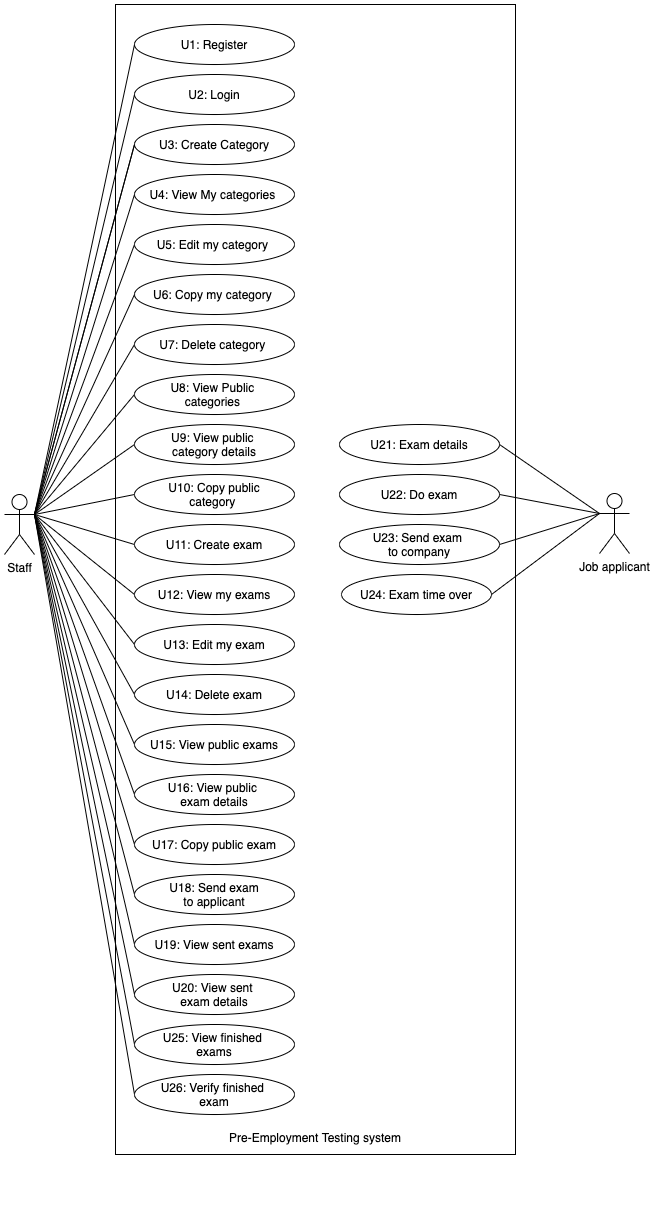
\includegraphics[width=0.78\columnwidth]{examaUseCaseDiagram .png}
  \caption{แผนภาพยูสเคสของระบบ}
  \label{Fig:examaUseCaseDiagram}
\end{figure}

\subsection{รายละเอียดการทำงานในแต่ละยูสเคศ (Use Case Description)}

\subsubsection{รายละเอียดยูสเคส ลงทะเบียน}

\begin{table}[H]
  \begin{tabular}{|l|l|l|} 
  \hline
  Use Case No:                                      & \multicolumn{2}{l|}{1}\\ 
  \hline
  Use Case Name:                                    & \multicolumn{2}{l|}{ลงทะเบียน}\\
  \hline
  Use Case~Scenario:                                & \multicolumn{2}{l|}{ผู้ใช้ลงทะเบียนกับระบบ}\\ 
  \hline
  \vcell{Triggering Event:}                         & \multicolumn{2}{l|}{\vcell{\begin{tabular}[b]{@{}l@{}}เมื่อผู้ใช้เข้าใช้งานเป็นครั้งแรก\end{tabular}}}\\[-\rowheight]
  \printcelltop                                     & \multicolumn{2}{l|}{\printcellmiddle}\\
  \hline
  Brief Description:                                & \multicolumn{2}{l|}{สำหรับให้ผู้ใช้ลงทะเบียนเข้าสู้ระบบ}\\ 
  \hline
  Actors:                                           & \multicolumn{2}{l|}{พนักงาน}\\ 
  \hline
  Related Use Cases:                                & \multicolumn{2}{l|}{-}\\ 
  \hline
  Stakeholders:                                     & \multicolumn{2}{l|}{-}\\ 
  \hline
  Pre - Conditions:                                 & \multicolumn{2}{l|}{-}\\ 
  \hline
  Post - Conditions:                                & \multicolumn{2}{l|}{ผู้ใช้สามารถเข้าใช้งานระบบได้}\\ 
  \hline
  Flow of Events:                                   & \multicolumn{1}{c|}{ผู้ใช้} & \multicolumn{1}{c|}{ระบบ}\\  
  \cline{2-3}
                                                    & \vcell{\begin{tabular}[b]{m{0.28\linewidth}}
                                                      1.ผู้ใช้เลือกลงทะเบียน\\\\\\
                                                      3.ผู้ใช้ทำการกรอกชื่อ-\\นามสกุล,อีเมล,รหัสผ่าน \\และยืนยันรหัสผ่าน แล้ว\\ทำการคลิกลงทะเบียน\\\\\\
                                                      5.ผู้ใช้งานได้รับอีเมล แล้ว\\ทำการคลิกลิงค์เว็บไซต์\\\\\\\\
                                                      \end{tabular}}
                                                    & \vcell{\begin{tabular}[b]{m{0.28\linewidth}}
                                                      \\
                                                      2.ระบบแสดงแบบฟอร์มให้กรอกข้อมูล\\\\\\\\\\
                                                      4.ระบบทำการส่งอีเมลให้ผู้\\ใช้เพื่อทำการยืนยันอีเมล\\\\\\
                                                      6.ระบบทำการยืนยันอีเมล\\ แล้วแสดงหน้าจอหลักของผู้ใช้งาน
                                                      \end{tabular}}\\[-\rowheight]
                                                    & \printcelltop & \printcelltop\\ 
  \hline
  \vcell{Exception Conditions:}                     & \multicolumn{2}{l|}{\vcell{\begin{tabular}[b]{@{}l@{}}- ผู้ใช้กรอกรายละเอียดไม่ครบถ้วน หรือไม่ตรงเงื่อนไข\\- ผู้ใช้ไม่ได้ทำการยืนยันอีเมล\\- ผู้ใช้กรอกอีเมลที่ไม่มีอยู่จริง\\- ผู้ใช้กรอกออีเมลที่ผู้ใช้งานไม่สามารถเข้าใช้อีเมลนั้นได้\end{tabular}}}\\[-\rowheight]
  \printcelltop                                     & \multicolumn{2}{l|}{\printcellmiddle}\\
  \hline
  \end{tabular}
  \caption{รายละเอียดยูสเคส ลงทะเบียน}
  \label{Table:register}
\end{table}

\subsubsection{รายละเอียดยูสเคส เข้าสู่ระบบ}

\begin{table}[H]
  \begin{tabular}{|l|l|l|} 
  \hline
  Use Case No:                                      & \multicolumn{2}{l|}{2}\\ 
  \hline
  Use Case Name:                                    & \multicolumn{2}{l|}{เข้าสู่ระบบ}\\
  \hline
  Use Case~Scenario:                                & \multicolumn{2}{l|}{ผู้ใช้ต้องการเข้าสู่ระบบ}\\ 
  \hline
  \vcell{Triggering Event:}                         & \multicolumn{2}{l|}{\vcell{\begin{tabular}[b]{@{}l@{}}- เมื่อผู้ใช้ต้องการเข้าใช้งานระบบ\\- ผู้ใช้เข้าเว็ปแอพพลิเคชั่นโดยที่ยังไม่เข้าใช้งานระบบ\end{tabular}}}\\[-\rowheight]
  \printcelltop                                     & \multicolumn{2}{l|}{\printcellmiddle}\\
  \hline
  Brief Description:                                & \multicolumn{2}{l|}{สำหรับให้ผู้ใช้เข้าสู่ระบบเพื่อเข้าใช้งานเว็ปแอปพลิเคชั่น}\\ 
  \hline
  Actors:                                           & \multicolumn{2}{l|}{พนักงาน}\\ 
  \hline
  Related Use Cases:                                & \multicolumn{2}{l|}{ลงทะเบียน}\\ 
  \hline
  Stakeholders:                                     & \multicolumn{2}{l|}{-}\\ 
  \hline
  Pre - Conditions:                                 & \multicolumn{2}{l|}{ผู้ใช้ต้องทำการลงทะเบียนและยืนยันตัวตนผ่านอีเมลเรียบร้อยแล้ว}\\ 
  \hline
  Post - Conditions:                                & \multicolumn{2}{l|}{ระบบแสดงหน้าจอสำหรับผู้ใช้งาน}\\ 
  \hline
  Flow of Events:                                   & \multicolumn{1}{c|}{ผู้ใช้} & \multicolumn{1}{c|}{ระบบ}\\  
  \cline{2-3}
                                                    & \vcell{\begin{tabular}[b]{m{0.28\linewidth}}
                                                      1.ผู้ใช้เข้าหน้าเว็ปโดยที่ยังไม่ได้ทำการเข้าสู้ระบบ\\\\\\
                                                      3.ผู้ใช้ทำการกรอกอีเมล และรหัสผ่านแล้วทำการคลิกเข้าสู่ระบบ หรือกด Enter บนแป้นพิมพ์\\\\\\
                                                      \end{tabular}}
                                                    & \vcell{\begin{tabular}[b]{m{0.28\linewidth}}
                                                      \\\\
                                                      2.ระบบแสดงแบบฟอร์มให้กรอกข้อมูล\\\\\\\\\\
                                                      4.ระบบแสดงหน้าจอหลักของผู้ใช้งาน
                                                      \end{tabular}}\\[-\rowheight]
                                                    & \printcelltop & \printcelltop\\ 
  \hline
  \vcell{Exception Conditions:}                     & \multicolumn{2}{l|}{\vcell{\begin{tabular}[b]{@{}l@{}}ผู้ใช้กรอกอีเมล หรือรหัสผ่านผิด\end{tabular}}}\\[-\rowheight]
  \printcelltop                                     & \multicolumn{2}{l|}{\printcellmiddle}\\
  \hline
  \end{tabular}
  \caption{รายละเอียดยูสเคส เข้าสู่ระบบ}
  \label{Table:login}
\end{table}

\subsubsection{รายละเอียดยูสเคส สร้างหมวดหมู่คำถาม}

\begin{table}[H]
  \begin{tabular}{|l|l|l|} 
  \hline
  Use Case No:                                      & \multicolumn{2}{l|}{3}\\ 
  \hline
  Use Case Name:                                    & \multicolumn{2}{l|}{สร้างหมวดหมู่คำถาม}\\
  \hline
  Use Case~Scenario:                                & \multicolumn{2}{l|}{ผู้ใช้ต้องการงหมวดหมู่คำถาม}\\
  \hline
  \vcell{Triggering Event:}                         & \multicolumn{2}{l|}{\vcell{\begin{tabular}[b]{@{}l@{}}เมื่อผู้ใช้ต้องการสร้างหมวดหมู่คำถาม ไว้ใช้ในข้อสอบของ\\ตนเอง หรือให้พนักงานคนอื่นใช้\end{tabular}}}\\[-\rowheight]
  \printcelltop                                     & \multicolumn{2}{l|}{\printcellmiddle}\\
  \hline
  \vcell{Brief Description:}                        & \multicolumn{2}{l|}{\vcell{\begin{tabular}[b]{@{}l@{}}สำหรับให้ผู้ใช้ ออกข้อสอบโดยแบ่งแยกตามแต่ละหมวดหมู่ เช่น\\คณิตศาสตร์, โปรแกรมมิ่ง หรือ แบบทดสอบสติปัญญา โดยมีชนิด\\คำถามแบ่งออกเป็น อัตนัย, ปรนัย และคำถามที่มีไฟล์แนบ\end{tabular}}}\\[-\rowheight]
  \printcelltop                                     & \multicolumn{2}{l|}{\printcellmiddle}\\
  \hline
  Actors:                                           & \multicolumn{2}{l|}{พนักงาน}\\ 
  \hline
  Related Use Cases:                                & \multicolumn{2}{l|}{เข้าสู่ระบบ}\\ 
  \hline
  Stakeholders:                                     & \multicolumn{2}{l|}{-}\\ 
  \hline
  Pre - Conditions:                                 & \multicolumn{2}{l|}{ผู้ใช้ต้องทำการเข้าสู่ระบบ}\\ 
  \hline
  \vcell{Post - Conditions:}                        & \multicolumn{2}{l|}{\vcell{\begin{tabular}[b]{@{}l@{}}ผู้ใช้มีหมวดหมู่คำถามที่ตนเองสร้างขึ้น และแสดงหน้าหมวด\\หมู่ทั้งหมดของผู้ใช้\end{tabular}}}\\[-\rowheight]
  \printcelltop                                     & \multicolumn{2}{l|}{\printcellmiddle}\\
  \hline
  Flow of Events:                                   & \multicolumn{1}{c|}{ผู้ใช้} & \multicolumn{1}{c|}{ระบบ}\\  
  \cline{2-3}
                                                    & \vcell{\begin{tabular}[b]{m{0.28\linewidth}}
                                                      1.ไปที่หน้าสร้างหมวดหมู่\\\\\\
                                                      3.ผู้ใช้กรอกชื่อหมวดหมู่\\และกรอกหัวเรื่อง\\
                                                      4.สร้างคำถามภายใต้ หมวดหมู่นั้นโดยสามารถเลือก\\ระดับความยาก และประเภทของคำถาม แล้วทำการคลิกสร้างหมวดหมู่\\\\\\\\                                                
                                                      \end{tabular}}
                                                    & \vcell{\begin{tabular}[b]{m{0.28\linewidth}}
                                                      \\
                                                      2.ระบบแสดงหน้าสร้าง\\หมวดหมู่คำถาม\\\\\\\\\\\\\\\\
                                                      5.ระบบทำการสร้างหมดหมู่คำถาม แล้วแสดงหน้าหมวด\\หมู่คำถามทั้งหมดของผู้ใช้
                                                      \end{tabular}}\\[-\rowheight]
                                                    & \printcelltop & \printcelltop\\ 
  \hline
  \vcell{Exception Conditions:}                     & \multicolumn{2}{l|}{\vcell{\begin{tabular}[b]{@{}l@{}}- ผู้ใช้กรอกขื่อหมวดหมู่ซ้ำกับ หมวดหมู่ที่ตนเองมีอยู่แล้ว\\- ผู้ใช้กรอกข้อมูลไม่ครบ ตามฟอร์มที่ให้กรอก\\- ไฟล์ที่แนบมามีขนาดใหญ่เกินที่กำหนด หรือประเภทของไฟล์ไม่\\\hspace{0.22cm}ถูกต้อง\end{tabular}}}\\[-\rowheight]
  \printcelltop                                     & \multicolumn{2}{l|}{\printcellmiddle}\\
  \hline
  \end{tabular}
  \caption{รายละเอียดยูสเคส สร้างหมวดหมู่คำถาม}
  \label{Table:createCategory}
\end{table}

\subsubsection{รายละเอียดยูสเคส ดูหมวดหมู่คำถามของผู้ใช้}

\begin{table}[H]
  \begin{tabular}{|l|l|l|} 
  \hline
  Use Case No:                                      & \multicolumn{2}{l|}{4}\\ 
  \hline
  Use Case Name:                                    & \multicolumn{2}{l|}{ดูหมวดหมู่คำถามของผู้ใช้}\\
  \hline
  Use Case~Scenario:                                & \multicolumn{2}{l|}{ผู้ใช้ต้องการดูหมวดหมู่คำถามของตนเอง}\\ 
  \hline
  \vcell{Triggering Event:}                         & \multicolumn{2}{l|}{\vcell{\begin{tabular}[b]{@{}l@{}}- เมื่อผู้ใช้ต้องการดูหมวดหมู่คำถามของตนเอง\\- เมื่อผู้ใช้สร้างประเภทของข้อสอบสำเร็จ หน้าเว็ปจะทำการไป\\\hspace{0.22cm}แสดงผลที่หน้าหมวดหมู่คำถามทั้งหมเของผู้ใช้\end{tabular}}}\\[-\rowheight]
  \printcelltop                                     & \multicolumn{2}{l|}{\printcellmiddle}\\
  \hline
  \vcell{Brief Description:}                        & \multicolumn{2}{l|}{\vcell{\begin{tabular}[b]{@{}l@{}}สำหรับให้ผู้ใช้งานดูหมวดหมู่คำถามที่ตนเองสร้างขึ้น หรือ\\หมวดหมู่คำถามที่คัดลอกมาจากหมวดหมู่สาธารณะ\end{tabular}}}\\[-\rowheight]
  \printcelltop                                     & \multicolumn{2}{l|}{\printcellmiddle}\\
  \hline
  Actors:                                           & \multicolumn{2}{l|}{พนักงาน}\\ 
  \hline
  \vcell{Related Use Cases:}                        & \multicolumn{2}{l|}{\vcell{\begin{tabular}[b]{@{}l@{}}เข้าสู่ระบบ, สร้างหมวดหมู่คำถาม, คัดลอกหมวดหมู่คำถาม\\จากหมวดหมู่คำถามสาธารณะ\end{tabular}}}\\[-\rowheight]
  \printcelltop                                     & \multicolumn{2}{l|}{\printcellmiddle}\\
  \hline
  Stakeholders:                                     & \multicolumn{2}{l|}{-}\\ 
  \hline
  \vcell{Pre - Conditions:}                         & \multicolumn{2}{l|}{\vcell{\begin{tabular}[b]{@{}l@{}}- ผู้ใช้ต้องทำการเข้าสู่ระบบ\\- สร้างหมวดหมู่คำถาม หรือคัดลอกหมวดหมู่คำถามจาก\\\hspace{0.22cm}หมวดหมู่คำถามสาธารณะ\end{tabular}}}\\[-\rowheight]
  \printcelltop                                     & \multicolumn{2}{l|}{\printcellmiddle}\\
  \hline
  \vcell{Post - Conditions:}                        & \multicolumn{2}{l|}{\vcell{\begin{tabular}[b]{@{}l@{}}แสดงหน้าหมวดหมู่ทั้งหมดของผู้ใช้\end{tabular}}}\\[-\rowheight]
  \printcelltop                                     & \multicolumn{2}{l|}{\printcellmiddle}\\
  \hline
  Flow of Events:                                   & \multicolumn{1}{c|}{ผู้ใช้} & \multicolumn{1}{c|}{ระบบ}\\  
  \cline{2-3}
                                                    & \vcell{\begin{tabular}[b]{m{0.28\linewidth}}
                                                      1.ไปที่หน้าดูหมวดหมู่คำ\\ถามของผู้ใช้                                            
                                                      \end{tabular}}
                                                    & \vcell{\begin{tabular}[b]{m{0.28\linewidth}}
                                                      \\\\
                                                      2.ระบบแสดงหมวดหมู่\\ทั้งหมดของผู้ใช้
                                                      \end{tabular}}\\[-\rowheight]
                                                    & \printcelltop & \printcelltop\\ 
  \hline
  \vcell{Exception Conditions:}                     & \multicolumn{2}{l|}{\vcell{\begin{tabular}[b]{@{}l@{}}ผู้ใช้ไม่มีหมวดหมู่คำถาม\end{tabular}}}\\[-\rowheight]
  \printcelltop                                     & \multicolumn{2}{l|}{\printcellmiddle}\\
  \hline
  \end{tabular}
  \caption{รายละเอียดยูสเคส ดูหมวดหมู่คำถามของผู้ใช้}
  \label{Table:viewMyCategory}
\end{table}

\subsubsection{รายละเอียดยูสเคส แก้ไขหมวดหมู่คำถามของผู้ใช้}

\begin{table}[H]
  \begin{tabular}{|l|l|l|} 
  \hline
  Use Case No:                                      & \multicolumn{2}{l|}{5}\\ 
  \hline
  Use Case Name:                                    & \multicolumn{2}{l|}{แก้ไขหมวดหมู่คำถามของผู้ใช้}\\
  \hline
  Use Case~Scenario:                                & \multicolumn{2}{l|}{ผู้ใช้ต้องการแก้ไขหมวดหมู่คำถามของตนเอง}\\ 
  \hline
  \vcell{Triggering Event:}                         & \multicolumn{2}{l|}{\vcell{\begin{tabular}[b]{@{}l@{}}เมื่อผู้ใช้ต้องการแก้ไขรายละเอียดในหมวดหมู่คำถาม เช่นเพิ่มคำ\\ถาม, แก้ไขคำถาม หรือแก้ไขชื่อหมวดหมู่\end{tabular}}}\\[-\rowheight]
  \printcelltop                                     & \multicolumn{2}{l|}{\printcellmiddle}\\
  \hline
  \vcell{Brief Description:}                        & \multicolumn{2}{l|}{\vcell{\begin{tabular}[b]{@{}l@{}}สำหรับให้ผู้ใช้งานแก้ไขรายละเอียดต่างๆในหมวดหมู่คำถาม\end{tabular}}}\\[-\rowheight]
  \printcelltop                                     & \multicolumn{2}{l|}{\printcellmiddle}\\
  \hline
  Actors:                                           & \multicolumn{2}{l|}{พนักงาน}\\ 
  \hline
  \vcell{Related Use Cases:}                        & \multicolumn{2}{l|}{\vcell{\begin{tabular}[b]{@{}l@{}}เข้าสู่ระบบ, สร้างหมวดหมู่คำถาม, คัดลอกหมวดหมู่คำถาม\\จากหมวดหมู่คำถามสาธารณะ\end{tabular}}}\\[-\rowheight]
  \printcelltop                                     & \multicolumn{2}{l|}{\printcellmiddle}\\
  \hline
  Stakeholders:                                     & \multicolumn{2}{l|}{-}\\ 
  \hline
  \vcell{Pre - Conditions:}                         & \multicolumn{2}{l|}{\vcell{\begin{tabular}[b]{@{}l@{}}- ผู้ใช้ต้องทำการเข้าสู่ระบบ\\- สร้างหมวดหมู่คำถาม หรือคัดลอกหมวดหมู่คำถามจาก\\\hspace{0.22cm}หมวดหมู่คำถามสาธารณะ\end{tabular}}}\\[-\rowheight]
  \printcelltop                                     & \multicolumn{2}{l|}{\printcellmiddle}\\
  \hline
  \vcell{Post - Conditions:}                        & \multicolumn{2}{l|}{\vcell{\begin{tabular}[b]{@{}l@{}}แสดงหน้าหมวดหมู่ทั้งหมดของผู้ใช้\end{tabular}}}\\[-\rowheight]
  \printcelltop                                     & \multicolumn{2}{l|}{\printcellmiddle}\\
  \hline
  Flow of Events:                                   & \multicolumn{1}{c|}{ผู้ใช้} & \multicolumn{1}{c|}{ระบบ}\\  
  \cline{2-3}
                                                    & \vcell{\begin{tabular}[b]{m{0.28\linewidth}}
                                                      1.ไปที่หน้าดูหมวดหมู่คำ\\ถามของผู้ใช้\\\\\\
                                                      3.คลิกที่หมวดหมู่คำถาม\\ที่ต้องการแก้ไข\\\\\\
                                                      5.ผู้ใช้ทำการแก้ไขข้อมูล\\ต่างๆในประเภทที่ต้องการ\\ แล้วทำการคลิกยืนยันการ\\แก้ไข\\\\\\\\
                                                      \end{tabular}}
                                                    & \vcell{\begin{tabular}[b]{m{0.28\linewidth}}
                                                      \\\\
                                                      2.ระบบแสดงหมวดหมู่\\ทั้งหมดของผู้ใช้\\\\\\
                                                      4.ระบบแสดงหน้าแก้ไข\\หมวดหมู่นั้นๆ\\\\\\\\\\
                                                      6.ระบบทำการแก้ไขข้อมูล\\
                                                      7.ระบบแสดงหน้าหมวดหมู่ทั้งหมดของผู้ใช้\\
                                                      \end{tabular}}\\[-\rowheight]
                                                    & \printcelltop & \printcelltop\\ 
  \hline
  \vcell{Exception Conditions:}                     & \multicolumn{2}{l|}{\vcell{
                                                        \begin{tabular}[b]{@{}l@{}}
                                                          - ผู้ใช้กรอกชื่อหมวดหมู่ซ้ำกับ หมวดหมู่ที่ตนเองมีอยู่แล้ว\\
                                                          - ผู้ใช้กรอกรายละเอียดไม่ครบถ้วน หรือไม่ตรงเงื่อนไข\\
                                                          - ไฟล์ที่แนบมามีขนาดใหญ่เกินที่กำหนด หรือประเภทของไฟล์\\\hspace{0.22cm}ไม่ถูกต้อง\\
                                                          - สามารถแก้ไขได้เฉพาะคำตอบ หากข้อสอบเคยถูกใช้ไปแล้ว
                                                        \end{tabular}}}\\[-\rowheight]
  \printcelltop                                     & \multicolumn{2}{l|}{\printcellmiddle}\\
  \hline
  \end{tabular}
  \caption{รายละเอียดยูสเคส แก้ไขหมวดหมู่คำถามของผู้ใช้}
  \label{Table:editMyCategory}
\end{table}

\subsubsection{รายละเอียดยูสเคส คัดลอกหมวดหมู่คำถามของผู้ใช้}

\begin{table}[H]
  \begin{tabular}{|l|l|l|} 
  \hline
  Use Case No:                                      & \multicolumn{2}{l|}{6}\\ 
  \hline
  Use Case Name:                                    & \multicolumn{2}{l|}{คัดลอกหมวดหมู่คำถามของผู้ใช้}\\
  \hline
  Use Case~Scenario:                                & \multicolumn{2}{l|}{ผู้ใช้ต้องการคัดลอกหมวดหมู่คำถามของตนเอง}\\ 
  \hline
  \vcell{Triggering Event:}                         & \multicolumn{2}{l|}{\vcell{\begin{tabular}[b]{@{}l@{}}เมื่อผู้ใช้ต้องการแก้ไขหมวดหมู่คำถามที่ถูกส่งให้ผู้สมัครงาน\\แล้ว ทำให้ไม่สามารถแก้ไขหมวดหมู่เดิมได้ หรือต้องการคัดลอก\\หมวดหมู่มาแก้ไข โดยที่ไม่ต้องการให้กระทบหมวดหมู่เดิม\end{tabular}}}\\[-\rowheight]
  \printcelltop                                     & \multicolumn{2}{l|}{\printcellmiddle}\\
  \hline
  \vcell{Brief Description:}                        & \multicolumn{2}{l|}{\vcell{\begin{tabular}[b]{@{}l@{}}สำหรับให้ผู้ใช้งานคัดลอกหมวดหมู่คำถามของตนเอง\end{tabular}}}\\[-\rowheight]
  \printcelltop                                     & \multicolumn{2}{l|}{\printcellmiddle}\\
  \hline
  Actors:                                           & \multicolumn{2}{l|}{พนักงาน}\\ 
  \hline
  \vcell{Related Use Cases:}                        & \multicolumn{2}{l|}{\vcell{\begin{tabular}[b]{@{}l@{}}เข้าสู่ระบบ, สร้างหมวดหมู่คำถาม, ส่งข้อสอบให้ผู้สมัคร\end{tabular}}}\\[-\rowheight]
  \printcelltop                                     & \multicolumn{2}{l|}{\printcellmiddle}\\
  \hline
  Stakeholders:                                     & \multicolumn{2}{l|}{-}\\ 
  \hline
  \vcell{Pre - Conditions:}                         & \multicolumn{2}{l|}{\vcell{\begin{tabular}[b]{@{}l@{}}- ผู้ใช้ต้องทำการเข้าสู่ระบบ\\- สร้างหมวดหมู่คำถาม หรือคัดลอกหมวดหมู่คำถามจาก\\\hspace{0.22cm}หมวดหมู่คำถามสาธารณะ\end{tabular}}}\\[-\rowheight]
  \printcelltop                                     & \multicolumn{2}{l|}{\printcellmiddle}\\
  \hline
  \vcell{Post - Conditions:}                        & \multicolumn{2}{l|}{\vcell{\begin{tabular}[b]{@{}l@{}}ระบบทำการคัดลอกหหมวดหมู่คำถามที่ผู้ใช้ต้องการ\end{tabular}}}\\[-\rowheight]
  \printcelltop                                     & \multicolumn{2}{l|}{\printcellmiddle}\\
  \hline
  Flow of Events:                                   & \multicolumn{1}{c|}{ผู้ใช้} & \multicolumn{1}{c|}{ระบบ}\\  
  \cline{2-3}
                                                    & \vcell{\begin{tabular}[b]{m{0.28\linewidth}}
                                                      1.ไปที่หน้าดูหมวดหมู่\\คำถามของผู้ใช้\\\\\\
                                                      3.คลิกปุ่มคักลอกที่หมวด\\หมู่ที่ต้องการคัดลอก\\\\\\
                                                      5.ผู้ใช้งานกดยืนยันการคัด\\ลอก\\\\\\
                                                      \end{tabular}}
                                                    & \vcell{\begin{tabular}[b]{m{0.28\linewidth}}
                                                      \\\\
                                                      2.ระบบแสดงหมวดหมู่\\ทั้งหมดของผู้ใช้\\\\\\
                                                      4.ระบบแสดงหน้ายืนยันการคัดลอก\\\\\\
                                                      6.ระบบทำการคัดลอกหมวดหมู่คำถามนั้น\\
                                                      \end{tabular}}\\[-\rowheight]
                                                    & \printcelltop & \printcelltop\\ 
  \hline
  \vcell{Exception Conditions:}                     & \multicolumn{2}{l|}{\vcell{
                                                        \begin{tabular}[b]{@{}l@{}}
                                                          ผู้ใช้ไม่มีหมวดหมู่คำถาม
                                                        \end{tabular}}}\\[-\rowheight]
  \printcelltop                                     & \multicolumn{2}{l|}{\printcellmiddle}\\
  \hline
  \end{tabular}
  \caption{รายละเอียดยูสเคส คัดลอกหมวดหมู่คำถามของผู้ใช้}
  \label{Table:copyMyCategory}
\end{table}

\subsubsection{รายละเอียดยูสเคส ลบหมวดหมู่คำถามของผู้ใช้}

\begin{table}[H]
  \begin{tabular}{|l|l|l|} 
  \hline
  Use Case No:                                      & \multicolumn{2}{l|}{7}\\ 
  \hline
  Use Case Name:                                    & \multicolumn{2}{l|}{ลบหมวดหมู่คำถามของผู้ใช้}\\
  \hline
  Use Case~Scenario:                                & \multicolumn{2}{l|}{ผู้ใช้ต้องการลบหมวดหมู่คำถามของตนเอง}\\ 
  \hline
  \vcell{Triggering Event:}                         & \multicolumn{2}{l|}{\vcell{\begin{tabular}[b]{@{}l@{}}เมื่อผู้ใช้ไม่ต้องการหมวดหมู่คำถามนั้นๆแล้ว\end{tabular}}}\\[-\rowheight]
  \printcelltop                                     & \multicolumn{2}{l|}{\printcellmiddle}\\
  \hline
  \vcell{Brief Description:}                        & \multicolumn{2}{l|}{\vcell{\begin{tabular}[b]{@{}l@{}}สำหรับให้ผู้ใช้งานลบหมวดหมู่คำถามออกจากหมวดหมู่คำถาม\\ของตนเอง\end{tabular}}}\\[-\rowheight]
  \printcelltop                                     & \multicolumn{2}{l|}{\printcellmiddle}\\
  \hline
  Actors:                                           & \multicolumn{2}{l|}{พนักงาน}\\ 
  \hline
  \vcell{Related Use Cases:}                        & \multicolumn{2}{l|}{\vcell{\begin{tabular}[b]{@{}l@{}}เข้าสู่ระบบ, สร้างหมวดหมู่คำถาม, คัดลอกหมวดหมู่คำถาม\\จากหมวดหมู่คำถามสาธารณะ, ข้อสอบของผู้ใช้\end{tabular}}}\\[-\rowheight]
  \printcelltop                                     & \multicolumn{2}{l|}{\printcellmiddle}\\
  \hline
  Stakeholders:                                     & \multicolumn{2}{l|}{-}\\ 
  \hline
  \vcell{Pre - Conditions:}                         & \multicolumn{2}{l|}{\vcell{\begin{tabular}[b]{@{}l@{}}- ผู้ใช้ต้องทำการเข้าสู่ระบบ\\- สร้างหมวดหมู่คำถาม หรือคัดลอกหมวดหมู่คำถามจาก\\\hspace{0.22cm}หมวดหมู่สาธารณะ\end{tabular}}}\\[-\rowheight]
  \printcelltop                                     & \multicolumn{2}{l|}{\printcellmiddle}\\
  \hline
  \vcell{Post - Conditions:}                        & \multicolumn{2}{l|}{\vcell{\begin{tabular}[b]{@{}l@{}}ระบบลบหมวดหมู่คำถามของผู้ใช้\end{tabular}}}\\[-\rowheight]
  \printcelltop                                     & \multicolumn{2}{l|}{\printcellmiddle}\\
  \hline
  Flow of Events:                                   & \multicolumn{1}{c|}{ผู้ใช้} & \multicolumn{1}{c|}{ระบบ}\\  
  \cline{2-3}
                                                    & \vcell{\begin{tabular}[b]{m{0.28\linewidth}}
                                                      1.ไปที่หน้าดูหมวดหมู่คำ\\ถามของผู้ใช้\\\\\\
                                                      3.คลิกที่รูปถึงขยะของ\\หมวดหมู่คำถามที่ต้องการลบ\\\\\\\\
                                                      5.ผู้ใช้ทำการยืนยันการลบ\\\\\\
                                                      \end{tabular}}
                                                    & \vcell{\begin{tabular}[b]{m{0.28\linewidth}}
                                                      \\\\
                                                      2.ระบบแสดงหมวดหมู่\\ทั้งหมดของผู้ใช้\\\\\\\\
                                                      4.ระบบทำการแสดง\\หน้าต่างข้อความยืนยัน\\การลบ\\\\
                                                      6.ระบบทำการลบหมวดหมู่คำถามที่ผู้ใช้ต้องการลบ\\
                                                      \end{tabular}}\\[-\rowheight]
                                                    & \printcelltop & \printcelltop\\ 
  \hline
  \vcell{Exception Conditions:}                     & \multicolumn{2}{l|}{\vcell{
                                                        \begin{tabular}[b]{@{}l@{}}
                                                          - ผู้ใช้ไม่ทำการยืนยันการลบ\\
                                                          - หมวดหมู่คำถามที่ต้องการลบ ถูกใช้งานอยู่ในข้อสอบ ทำให้ไม่\\
                                                          \hspace{0.22cm}สามารถลบได้
                                                        \end{tabular}}}\\[-\rowheight]
  \printcelltop                                     & \multicolumn{2}{l|}{\printcellmiddle}\\
  \hline
  \end{tabular}
  \caption{รายละเอียดยูสเคส ลบหมวดหมู่คำถามของผู้ใช้}
  \label{Table:deleteCategory}
\end{table}

\subsubsection{รายละเอียดยูสเคส ดูหมวดหมู่คำถามสาธารณะ}

\begin{table}[H]
  \begin{tabular}{|l|l|l|} 
  \hline
  Use Case No:                                      & \multicolumn{2}{l|}{8}\\ 
  \hline
  Use Case Name:                                    & \multicolumn{2}{l|}{ดูหมวดหมู่คำถามสาธารณะ}\\
  \hline
  Use Case~Scenario:                                & \multicolumn{2}{l|}{ผู้ใช้ต้องการดูหมวดหมู่คำถามสาธารณะ}\\ 
  \hline
  \vcell{Triggering Event:}                         & \multicolumn{2}{l|}{\vcell{
                                                        \begin{tabular}[b]{@{}l@{}}
                                                          - เมื่อผู้ใช้ต้องการดูหมวดหมู่คำถามสาธารณะ\\
                                                          - เมื่อผู้ใช้ต้องการนำหมวดหมู่คำถามสาธารณะไปใช้ในข้อสอบ\\
                                                          \hspace{0.22cm}ของตนเอง
                                                        \end{tabular}}}\\[-\rowheight]
  \printcelltop                                     & \multicolumn{2}{l|}{\printcellmiddle}\\
  \hline
  \vcell{Brief Description:}                        & \multicolumn{2}{l|}{\vcell{\begin{tabular}[b]{@{}l@{}}สำหรับให้ผู้ใช้ดูว่ามีหมวดหมู่คำถามสาธารณะใดบ้างที่อยู่ใน\\ระบบและสามารถคัดลอกไปใช้ได้\end{tabular}}}\\[-\rowheight]
  \printcelltop                                     & \multicolumn{2}{l|}{\printcellmiddle}\\
  \hline
  Actors:                                           & \multicolumn{2}{l|}{พนักงาน}\\ 
  \hline
  \vcell{Related Use Cases:}                        & \multicolumn{2}{l|}{\vcell{\begin{tabular}[b]{@{}l@{}}เข้าสู่ระบบ\end{tabular}}}\\[-\rowheight]
  \printcelltop                                     & \multicolumn{2}{l|}{\printcellmiddle}\\
  \hline
  Stakeholders:                                     & \multicolumn{2}{l|}{-}\\ 
  \hline
  \vcell{Pre - Conditions:}                         & \multicolumn{2}{l|}{\vcell{\begin{tabular}[b]{@{}l@{}}ผู้ใช้ต้องทำการเข้าสู่ระบบ\end{tabular}}}\\[-\rowheight]
  \printcelltop                                     & \multicolumn{2}{l|}{\printcellmiddle}\\
  \hline
  \vcell{Post - Conditions:}                        & \multicolumn{2}{l|}{\vcell{\begin{tabular}[b]{@{}l@{}}ระบบแสดงหมวดหมูข้อสอบทั้งหมด ที่เป็นสาธารณะ\end{tabular}}}\\[-\rowheight]
  \printcelltop                                     & \multicolumn{2}{l|}{\printcellmiddle}\\
  \hline
  Flow of Events:                                   & \multicolumn{1}{c|}{ผู้ใช้} & \multicolumn{1}{c|}{ระบบ}\\  
  \cline{2-3}
                                                    & \vcell{\begin{tabular}[b]{m{0.28\linewidth}}
                                                      1.ไปที่หน้าดูหมวดหมู่\\คำถามสาธารณะ\\\\\\
                                                      \end{tabular}}
                                                    & \vcell{\begin{tabular}[b]{m{0.28\linewidth}}
                                                      \\\\
                                                      2.ระบบแสดงหมวดหมู่\\ทั้งหมดที่เป็นสาธารณะ
                                                      \end{tabular}}\\[-\rowheight]
                                                    & \printcelltop & \printcelltop\\ 
  \hline
  \vcell{Exception Conditions:}                     & \multicolumn{2}{l|}{\vcell{
                                                        \begin{tabular}[b]{@{}l@{}}
                                                          ไม่มีหมวดหมู่คำถามที่เป็นสาธารณะอยู่ในระบบ
                                                        \end{tabular}}}\\[-\rowheight]
  \printcelltop                                     & \multicolumn{2}{l|}{\printcellmiddle}\\
  \hline
  \end{tabular}
  \caption{รายละเอียดยูสเคส ดูหมวดหมู่คำถามสาธารณะ}
  \label{Table:viewPublicCategorires}
\end{table}

\subsubsection{รายละเอียดยูสเคส ดูรายละเอียดของหมวดหมู่คำถามสาธารณะ}

\begin{table}[H]
  \begin{tabular}{|l|l|l|} 
  \hline
  Use Case No:                                      & \multicolumn{2}{l|}{9}\\ 
  \hline
  Use Case Name:                                    & \multicolumn{2}{l|}{ดูรายละเอียดของหมวดหมู่คำถามสาธารณะ}\\
  \hline
  Use Case~Scenario:                                & \multicolumn{2}{l|}{ผู้ใช้ต้องการดูรายละเอียดในหมวดหมู่คำถามสาธารณะที่ต้องการ}\\ 
  \hline
  \vcell{Triggering Event:}                         & \multicolumn{2}{l|}{\vcell{
                                                        \begin{tabular}[b]{@{}l@{}}
                                                          - เมื่อผู้ใช้ต้องการดูรายละเอียดของหมวดหมู่คำถามสาธารณะ\\
                                                          - เมื่อผู้ใช้ต้องการนำหมวดหมู่คำถามสาธารณะนั้นๆไปใช้ใน\\
                                                          \hspace{0.22cm}ข้อสอบของตนเอง
                                                        \end{tabular}}}\\[-\rowheight]
  \printcelltop                                     & \multicolumn{2}{l|}{\printcellmiddle}\\
  \hline
  \vcell{Brief Description:}                        & \multicolumn{2}{l|}{\vcell{\begin{tabular}[b]{@{}l@{}}สำหรับให้ผู้ใช้ดูรายละเอียดของหมวดหมู่คำถามสาธารณะ ว่าใน\\หมวดหมู่นั้นมีคำถามอะไรบ้าง\end{tabular}}}\\[-\rowheight]
  \printcelltop                                     & \multicolumn{2}{l|}{\printcellmiddle}\\
  \hline
  Actors:                                           & \multicolumn{2}{l|}{พนักงาน}\\ 
  \hline
  \vcell{Related Use Cases:}                        & \multicolumn{2}{l|}{\vcell{\begin{tabular}[b]{@{}l@{}}เข้าสู่ระบบ, ดูหมวดหมู่คำถามสาธารณะ\end{tabular}}}\\[-\rowheight]
  \printcelltop                                     & \multicolumn{2}{l|}{\printcellmiddle}\\
  \hline
  Stakeholders:                                     & \multicolumn{2}{l|}{-}\\ 
  \hline
  \vcell{Pre - Conditions:}                         & \multicolumn{2}{l|}{\vcell{\begin{tabular}[b]{@{}l@{}}ผู้ใช้ต้องทำการเข้าสู่ระบบ\end{tabular}}}\\[-\rowheight]
  \printcelltop                                     & \multicolumn{2}{l|}{\printcellmiddle}\\
  \hline
  \vcell{Post - Conditions:}                        & \multicolumn{2}{l|}{\vcell{\begin{tabular}[b]{@{}l@{}}ระบบรายละเอียดของหมวดหมูข้อสอบนั้นๆ\end{tabular}}}\\[-\rowheight]
  \printcelltop                                     & \multicolumn{2}{l|}{\printcellmiddle}\\
  \hline
  Flow of Events:                                   & \multicolumn{1}{c|}{ผู้ใช้} & \multicolumn{1}{c|}{ระบบ}\\  
  \cline{2-3}
                                                    & \vcell{\begin{tabular}[b]{m{0.28\linewidth}}
                                                      1.ไปที่หน้าดูหมวดหมู่\\คำถามสาธารณะ\\\\\\
                                                      3.คลิกหมวดหมู่ที่ต้องการ\\ดูรายละเอียด\\
                                                      \end{tabular}}
                                                    & \vcell{\begin{tabular}[b]{m{0.28\linewidth}}
                                                      \\\\
                                                      2.ระบบแสดงหมวดหมู่\\ทั้งหมดที่เป็นสาธารณะ\\\\\\
                                                      4.ระบบแสดงรายละเอียด\\ของหมวดหมู่คำถามนั้น
                                                      \end{tabular}}\\[-\rowheight]
                                                    & \printcelltop & \printcelltop\\ 
  \hline
  \vcell{Exception Conditions:}                     & \multicolumn{2}{l|}{\vcell{
                                                        \begin{tabular}[b]{@{}l@{}}
                                                          ไม่มีหมวดหมู่คำถามที่เป็นสาธารณะอยู่ในระบบ
                                                        \end{tabular}}}\\[-\rowheight]
  \printcelltop                                     & \multicolumn{2}{l|}{\printcellmiddle}\\
  \hline
  \end{tabular}
  \caption{รายละเอียดยูสเคส ดูรายละเอียดของหมวดหมู่คำถามสาธารณะ}
  \label{Table:viewPublicCategoriryDetails}
\end{table}

\subsubsection{รายละเอียดยูสเคส คัดลอกหมวดหมู่คำถามสาธารณะ}

\begin{table}[H]
  \begin{tabular}{|l|l|l|} 
  \hline
  Use Case No:                                      & \multicolumn{2}{l|}{10}\\ 
  \hline
  Use Case Name:                                    & \multicolumn{2}{l|}{คัดลอกหมวดหมู่คำถามสาธารณะ}\\
  \hline
  Use Case~Scenario:                                & \multicolumn{2}{l|}{ผู้ใช้ต้องการนำหมวดหมู่คำถามสาธารณะ}\\ 
  \hline
  \vcell{Triggering Event:}                         & \multicolumn{2}{l|}{\vcell{
                                                        \begin{tabular}[b]{@{}l@{}}
                                                          เมื่อผู้ใช้ต้องการนำหมวดหมู่คำถามสาธารณะนั้นๆ ไปใช้ในข้อ\\สอบของตนเอง
                                                        \end{tabular}}}\\[-\rowheight]
  \printcelltop                                     & \multicolumn{2}{l|}{\printcellmiddle}\\
  \hline
  \vcell{Brief Description:}                        & \multicolumn{2}{l|}{\vcell{\begin{tabular}[b]{@{}l@{}}สำหรับให้ผู้ใช้ทำการคัดลอกหมวดหมู่คำถามสาธารณะ ไปใช้ใน\\ข้อสอบของตนเอง\end{tabular}}}\\[-\rowheight]
  \printcelltop                                     & \multicolumn{2}{l|}{\printcellmiddle}\\
  \hline
  Actors:                                           & \multicolumn{2}{l|}{พนักงาน}\\ 
  \hline
  \vcell{Related Use Cases:}                        & \multicolumn{2}{l|}{\vcell{\begin{tabular}[b]{@{}l@{}}เข้าสู่ระบบ, ดูหมวดหมู่คำถามหมวดหมู่คำถามสาธารณะ\end{tabular}}}\\[-\rowheight]
  \printcelltop                                     & \multicolumn{2}{l|}{\printcellmiddle}\\
  \hline
  Stakeholders:                                     & \multicolumn{2}{l|}{-}\\ 
  \hline
  \vcell{Pre - Conditions:}                         & \multicolumn{2}{l|}{\vcell{\begin{tabular}[b]{@{}l@{}}ผู้ใช้ต้องทำการเข้าสู่ระบบ\end{tabular}}}\\[-\rowheight]
  \printcelltop                                     & \multicolumn{2}{l|}{\printcellmiddle}\\
  \hline
  \vcell{Post - Conditions:}                        & \multicolumn{2}{l|}{\vcell{\begin{tabular}[b]{@{}l@{}}ระบบทำการคักลอกหมวดหมู่สาธารณะที่ผู้ใช้ต้องการ ไปเก็บใน\\หมวดหมู่คำถามของตนเอง\end{tabular}}}\\[-\rowheight]
  \printcelltop                                     & \multicolumn{2}{l|}{\printcellmiddle}\\
  \hline
  Flow of Events:                                   & \multicolumn{1}{c|}{ผู้ใช้} & \multicolumn{1}{c|}{ระบบ}\\  
  \cline{2-3}
                                                    & \vcell{\begin{tabular}[b]{m{0.28\linewidth}}
                                                      1.ไปที่หน้าดูหมวดหมู่\\คำถามสาธารณะ\\\\\\
                                                      3.คลิกปุ่มคัดลอกที่หมวด\\หมู่ที่ต้องการ\\\\\\\\\\
                                                      \end{tabular}}
                                                    & \vcell{\begin{tabular}[b]{m{0.28\linewidth}}
                                                      \\\\
                                                      2.ระบบแสดงหมวดหมู่\\ทั้งหมดที่เป็นสาธารณะ\\\\\\
                                                      4.ระบบทำการคัดลอกข้อมูลสาธารณะที่ต้องการ ไปเก็บในหมวดหมู่คำถามของตน\\เอง
                                                      \end{tabular}}\\[-\rowheight]
                                                    & \printcelltop & \printcelltop\\ 
  \hline
  \vcell{Exception Conditions:}                     & \multicolumn{2}{l|}{\vcell{
                                                        \begin{tabular}[b]{@{}l@{}}
                                                          ไม่มีหมวดหมู่คำถามที่เป็นสาธารณะอยู่ในระบบ
                                                        \end{tabular}}}\\[-\rowheight]
  \printcelltop                                     & \multicolumn{2}{l|}{\printcellmiddle}\\
  \hline
  \end{tabular}
  \caption{รายละเอียดยูสเคส คัดลอกหมวดหมู่คำถามสาธารณะ}
  \label{Table:copyPublicCategory}
\end{table}

\subsubsection{รายละเอียดยูสเคส สร้างข้อสอบ}

\begin{table}[H]
  \begin{tabular}{|l|l|l|} 
  \hline
  Use Case No:                                      & \multicolumn{2}{l|}{11}\\ 
  \hline
  Use Case Name:                                    & \multicolumn{2}{l|}{สร้างข้อสอบ}\\
  \hline
  Use Case~Scenario:                                & \multicolumn{2}{l|}{ผู้ใช้ต้องการสร้างข้อสอบ}\\ 
  \hline
  \vcell{Triggering Event:}                         & \multicolumn{2}{l|}{\vcell{
                                                        \begin{tabular}[b]{@{}l@{}}
                                                          เมื่อผู้ใช้ต้องการสร้างข้อสอบไปของตนเอง เพื่อนำไปทดสอบกับ\\ผู้สมัครงาน
                                                        \end{tabular}}}\\[-\rowheight]
  \printcelltop                                     & \multicolumn{2}{l|}{\printcellmiddle}\\
  \hline
  \vcell{Brief Description:}                        & \multicolumn{2}{l|}{\vcell{
                                                        \begin{tabular}[b]{@{}l@{}}
                                                          สำหรับผู้ใช้ที่ต้องการทำการออกข้อสอบ โดยการดึงคำถามจาก\\
                                                          ประเภทของข้อสอบ ตามจำนวนข้อและความยากที่ต้องการ เช่น\\
                                                          ต้องการคำถามหมวดหมู่ คณิตศาสตร์ ข้อระดับง่าย 2 ข้อ ข้อระดับ\\
                                                          ยาก 1 ข้อ และคำถามหมวดหมู่ ภาษาอังกฤษ ข้อระดับปลานกลาง\\
                                                          3 ข้อ สามารถกำหนดระยะเวลาในการทำข้อสอบ และวันหมดอายุ\\
                                                          ของข้อสอบได้
                                                        \end{tabular}}}\\[-\rowheight]
  \printcelltop                                     & \multicolumn{2}{l|}{\printcellmiddle}\\
  \hline
  Actors:                                           & \multicolumn{2}{l|}{พนักงาน}\\ 
  \hline
  \vcell{Related Use Cases:}                        & \multicolumn{2}{l|}{\vcell{\begin{tabular}[b]{@{}l@{}}เข้าสู่ระบบ, สร้างหมวดหมู่คำถาม, คัดลอกหมวดหมู่คำถาม\\สาธารณะ\end{tabular}}}\\[-\rowheight]
  \printcelltop                                     & \multicolumn{2}{l|}{\printcellmiddle}\\
  \hline
  Stakeholders:                                     & \multicolumn{2}{l|}{-}\\ 
  \hline
  \vcell{Pre - Conditions:}                         & \multicolumn{2}{l|}{\vcell{
                                                        \begin{tabular}[b]{@{}l@{}}
                                                          - ผู้ใช้ต้องทำการเข้าสู่ระบบ\\
                                                          - ผู้ใช้งานต้องสร้างหมวดหมู่คำถามของตนเอง หรือคัดลอก\\
                                                          \hspace{0.22cm}หมวดหมู่คำถามสาธารณะ
                                                        \end{tabular}}}\\[-\rowheight]
  \printcelltop                                     & \multicolumn{2}{l|}{\printcellmiddle}\\
  \hline
  \vcell{Post - Conditions:}                        & \multicolumn{2}{l|}{\vcell{\begin{tabular}[b]{@{}l@{}}ระบบทำการสร้างข้อสอบตามที่ผู้ใช้กำหนด\end{tabular}}}\\[-\rowheight]
  \printcelltop                                     & \multicolumn{2}{l|}{\printcellmiddle}\\
  \hline
  Flow of Events:                                   & \multicolumn{1}{c|}{ผู้ใช้} & \multicolumn{1}{c|}{ระบบ}\\  
  \cline{2-3}
                                                    & \vcell{\begin{tabular}[b]{m{0.28\linewidth}}
                                                      1.ไปที่หน้าสร้างข้อสอบ\\\\\\\\\\
                                                      3.เลือกหมวดหมู่คำถามที่\\ต้องการ แล้วเลือกระดับ\\ความยากและจำนวนข้อที่\\ต้องการในหมวดหมู่นั้นๆ\\ แล้วคลิกสร้างข้อสอบ\\\\\\
                                                      \end{tabular}}
                                                    & \vcell{\begin{tabular}[b]{m{0.28\linewidth}}
                                                      \\
                                                      2.ระบบแสดงหมดหมู่ของ\\ตนเองสำหรับเลือกใช้ใน\\ข้อสอบ และแสดงรายละ\\เอียดให้กรอก\\\\\\\\\\\\
                                                      4.ระบบทำการสร้างข้อสอบตามที่ผู้ใช้งานกำหนด
                                                      \end{tabular}}\\[-\rowheight]
                                                    & \printcelltop & \printcelltop\\ 
  \hline
  \vcell{Exception Conditions:}                     & \multicolumn{2}{l|}{\vcell{
                                                        \begin{tabular}[b]{@{}l@{}}
                                                          - ไม่มีหมวดหมู่คำถามของตนเอง\\
                                                          - ผู้ใช้กรอกรายละเอียดไม่ครบถ้วน หรือไม่ตรงเงื่อนไข
                                                        \end{tabular}}}\\[-\rowheight]
  \printcelltop                                     & \multicolumn{2}{l|}{\printcellmiddle}\\
  \hline
  \end{tabular}
  \caption{รายละเอียดยูสเคส สร้างข้อสอบ}
  \label{Table:createExam}
\end{table}

\subsubsection{รายละเอียดยูสเคส ดูข้อสอบทั้งหมดของตนเอง}

\begin{table}[H]
  \begin{tabular}{|l|l|l|} 
  \hline
  Use Case No:                                      & \multicolumn{2}{l|}{12}\\ 
  \hline
  Use Case Name:                                    & \multicolumn{2}{l|}{ดูข้อสอบทั้งหมดของตนเอง}\\
  \hline
  Use Case~Scenario:                                & \multicolumn{2}{l|}{ผู้ใช้ต้องการดูข้อสอบทั้งหมดของตนเอง}\\ 
  \hline
  \vcell{Triggering Event:}                         & \multicolumn{2}{l|}{\vcell{
                                                        \begin{tabular}[b]{@{}l@{}}
                                                          เมื่อผู้ใช้ต้องการดูว่าตนเองมีข้อสอบอะไรบ้าง
                                                        \end{tabular}}}\\[-\rowheight]
  \printcelltop                                     & \multicolumn{2}{l|}{\printcellmiddle}\\
  \hline
  \vcell{Brief Description:}                        & \multicolumn{2}{l|}{\vcell{
                                                        \begin{tabular}[b]{@{}l@{}}
                                                          สำหรับผู้ใช้ที่ดูข้อสอบที่ตนเองสร้างขึ้น หรือดูข้อสอบที่ทำการคัด\\ลอกมาจากข้อสอบสาธารณะ
                                                        \end{tabular}}}\\[-\rowheight]
  \printcelltop                                     & \multicolumn{2}{l|}{\printcellmiddle}\\
  \hline
  Actors:                                           & \multicolumn{2}{l|}{พนักงาน}\\ 
  \hline
  \vcell{Related Use Cases:}                        & \multicolumn{2}{l|}{\vcell{\begin{tabular}[b]{@{}l@{}}เข้าสู่ระบบ, สร้างข้อสอบ, คัดลอกข้อสอบจากสาธารณะ\end{tabular}}}\\[-\rowheight]
  \printcelltop                                     & \multicolumn{2}{l|}{\printcellmiddle}\\
  \hline
  Stakeholders:                                     & \multicolumn{2}{l|}{-}\\ 
  \hline
  \vcell{Pre - Conditions:}                         & \multicolumn{2}{l|}{\vcell{
                                                        \begin{tabular}[b]{@{}l@{}}
                                                          ผู้ใช้ต้องทำการเข้าสู่ระบบ
                                                        \end{tabular}}}\\[-\rowheight]
  \printcelltop                                     & \multicolumn{2}{l|}{\printcellmiddle}\\
  \hline
  \vcell{Post - Conditions:}                        & \multicolumn{2}{l|}{\vcell{\begin{tabular}[b]{@{}l@{}}ระบบทำการแสดงข้อสอบทั้งหมดของตนเอง\end{tabular}}}\\[-\rowheight]
  \printcelltop                                     & \multicolumn{2}{l|}{\printcellmiddle}\\
  \hline
  Flow of Events:                                   & \multicolumn{1}{c|}{ผู้ใช้} & \multicolumn{1}{c|}{ระบบ}\\  
  \cline{2-3}
                                                    & \vcell{\begin{tabular}[b]{m{0.28\linewidth}}
                                                      1.ไปที่หน้าดูข้อสอบทั้งหมดของตนเอง\\\\\\
                                                      \end{tabular}}
                                                    & \vcell{\begin{tabular}[b]{m{0.28\linewidth}}
                                                      \\\\
                                                      2.ระบบแสดงข้อสอบ\\ทั้งหมดของผู้ใช้
                                                      \end{tabular}}\\[-\rowheight]
                                                    & \printcelltop & \printcelltop\\ 
  \hline
  \vcell{Exception Conditions:}                     & \multicolumn{2}{l|}{\vcell{
                                                        \begin{tabular}[b]{@{}l@{}}
                                                          ไม่มีข้อสอบของตนเอง
                                                        \end{tabular}}}\\[-\rowheight]
  \printcelltop                                     & \multicolumn{2}{l|}{\printcellmiddle}\\
  \hline
  \end{tabular}
  \caption{รายละเอียดยูสเคส ดูข้อสอบทั้งหมดของตนเอง}
  \label{Table:viewMyExams}
\end{table}

\subsubsection{รายละเอียดยูสเคส แก้ไขข้อสอบของตนเอง}

\begin{table}[H]
  \begin{tabular}{|l|l|l|} 
  \hline
  Use Case No:                                      & \multicolumn{2}{l|}{13}\\ 
  \hline
  Use Case Name:                                    & \multicolumn{2}{l|}{แก้ไขข้อสอบของตนเอง}\\
  \hline
  Use Case~Scenario:                                & \multicolumn{2}{l|}{ผู้ใช้ต้องการแก้ไขข้อสอบของตนเอง}\\ 
  \hline
  \vcell{Triggering Event:}                         & \multicolumn{2}{l|}{\vcell{
                                                        \begin{tabular}[b]{@{}l@{}}
                                                          เมื่อผู้ใช้ต้องการแก้ไขข้อสอบที่ตนเองสร้างขึ้น หรือข้อสอบที่ทำ\\
                                                          การคัดสอกมาจากข้อสอบสาธารณะ
                                                        \end{tabular}}}\\[-\rowheight]
  \printcelltop                                     & \multicolumn{2}{l|}{\printcellmiddle}\\
  \hline
  \vcell{Brief Description:}                        & \multicolumn{2}{l|}{\vcell{
                                                        \begin{tabular}[b]{@{}l@{}}
                                                          สำหรับผู้ใช้ที่ต้องการแก้ไขข้อสอบ เช่น เพิ่มหรือลดจำนวนข้อและ\\ระดับความยากในหมวดหมู่คำถามนั้นๆ
                                                        \end{tabular}}}\\[-\rowheight]
  \printcelltop                                     & \multicolumn{2}{l|}{\printcellmiddle}\\
  \hline
  Actors:                                           & \multicolumn{2}{l|}{พนักงาน}\\ 
  \hline
  \vcell{Related Use Cases:}                        & \multicolumn{2}{l|}{\vcell{\begin{tabular}[b]{@{}l@{}}เข้าสู่ระบบ, สร้างข้อสอบ, คัดลอกข้อสอบจากสาธารณะ\end{tabular}}}\\[-\rowheight]
  \printcelltop                                     & \multicolumn{2}{l|}{\printcellmiddle}\\
  \hline
  Stakeholders:                                     & \multicolumn{2}{l|}{-}\\ 
  \hline
  \vcell{Pre - Conditions:}                         & \multicolumn{2}{l|}{\vcell{
                                                        \begin{tabular}[b]{@{}l@{}}
                                                          - ผู้ใช้ต้องทำการเข้าสู่ระบบ\\
                                                          - ผู้ใช้ต้องสร้างข้อสอบ หรือคัดลอกข้อสอบจากข้อสอบสาธารณะ
                                                        \end{tabular}}}\\[-\rowheight]
  \printcelltop                                     & \multicolumn{2}{l|}{\printcellmiddle}\\
  \hline
  \vcell{Post - Conditions:}                        & \multicolumn{2}{l|}{\vcell{\begin{tabular}[b]{@{}l@{}}ระบบทำการแก้ไขข้อสอบตามที่ผู้ใช้กำหนด\end{tabular}}}\\[-\rowheight]
  \printcelltop                                     & \multicolumn{2}{l|}{\printcellmiddle}\\
  \hline
  Flow of Events:                                   & \multicolumn{1}{c|}{ผู้ใช้} & \multicolumn{1}{c|}{ระบบ}\\  
  \cline{2-3}
                                                    & \vcell{\begin{tabular}[b]{m{0.28\linewidth}}
                                                      1.ไปที่หน้าดูข้อสอบทั้งหมดของตนเอง\\\\\\
                                                      3.เลือกข้อสอบที่ต้องการ\\แก้ไข\\\\\\
                                                      5.ทำการแก้ไขข้อสอบตามที่ต้องการ แล้วคลิกยืนยัน\\\\\\
                                                      \end{tabular}}
                                                    & \vcell{\begin{tabular}[b]{m{0.28\linewidth}}
                                                      \\\\
                                                      2.ระบบแสดงข้อสอบ\\ทั้งหมดของผู้ใช้\\\\\\
                                                      4.ระบบทำการแสดงราย\\ละเอียดของข้อสอบนั้น\\\\\\
                                                      6.ระบบทำการแก้ไขตามที่ผู้ใช้กำหนด
                                                      \end{tabular}}\\[-\rowheight]
                                                    & \printcelltop & \printcelltop\\ 
  \hline
  \vcell{Exception Conditions:}                     & \multicolumn{2}{l|}{\vcell{
                                                        \begin{tabular}[b]{@{}l@{}}
                                                          - ไม่มีข้อสอบของตนเอง\\
                                                          - ผู้ใช้มีการใช้ขื่อซ้ำกับข้อสอบของตนเองที่มีอยู่\\
                                                          - ผู้ใช้กรอกรายละเอียดไม่ครบถ้วน หรือไม่ตรงเงื่อนไข
                                                        \end{tabular}}}\\[-\rowheight]
  \printcelltop                                     & \multicolumn{2}{l|}{\printcellmiddle}\\
  \hline
  \end{tabular}
  \caption{รายละเอียดยูสเคส แก้ไขข้อสอบของตนเอง}
  \label{Table:editMyExam}
\end{table}

\subsubsection{รายละเอียดยูสเคส แก้ไขข้อสอบของตนเอง}

\begin{table}[H]
  \begin{tabular}{|l|l|l|} 
  \hline
  Use Case No:                                      & \multicolumn{2}{l|}{13}\\ 
  \hline
  Use Case Name:                                    & \multicolumn{2}{l|}{แก้ไขข้อสอบของตนเอง}\\
  \hline
  Use Case~Scenario:                                & \multicolumn{2}{l|}{ผู้ใช้ต้องการแก้ไขรายละเอียดข้อสอบของตนเอง}\\ 
  \hline
  \vcell{Triggering Event:}                         & \multicolumn{2}{l|}{\vcell{
                                                        \begin{tabular}[b]{@{}l@{}}
                                                          เมื่อผู้ใช้ต้องการแก้ไขรายละเอียดข้อสอบที่ตนเองสร้างขึ้น หรือ\\
                                                          ข้อสอบที่ทำการคัดสอกมาจากข้อสอบสาธารณะ
                                                        \end{tabular}}}\\[-\rowheight]
  \printcelltop                                     & \multicolumn{2}{l|}{\printcellmiddle}\\
  \hline
  \vcell{Brief Description:}                        & \multicolumn{2}{l|}{\vcell{
                                                        \begin{tabular}[b]{@{}l@{}}
                                                          สำหรับผู้ใช้ที่ต้องการแก้ไขรายละเอียดข้อสอบ เช่น เพิ่มหรือลด\\จำนวนข้อและระดับความยากในหมวดหมู่คำถามนั้นๆ
                                                        \end{tabular}}}\\[-\rowheight]
  \printcelltop                                     & \multicolumn{2}{l|}{\printcellmiddle}\\
  \hline
  Actors:                                           & \multicolumn{2}{l|}{พนักงาน}\\ 
  \hline
  \vcell{Related Use Cases:}                        & \multicolumn{2}{l|}{\vcell{\begin{tabular}[b]{@{}l@{}}เข้าสู่ระบบ, สร้างข้อสอบ, คัดลอกข้อสอบจากสาธารณะ\end{tabular}}}\\[-\rowheight]
  \printcelltop                                     & \multicolumn{2}{l|}{\printcellmiddle}\\
  \hline
  Stakeholders:                                     & \multicolumn{2}{l|}{-}\\ 
  \hline
  \vcell{Pre - Conditions:}                         & \multicolumn{2}{l|}{\vcell{
                                                        \begin{tabular}[b]{@{}l@{}}
                                                          - ผู้ใช้ต้องทำการเข้าสู่ระบบ\\
                                                          - ผู้ใช้ต้องสร้างข้อสอบ หรือคัดลอกข้อสอบจากข้อสอบสาธารณะ
                                                        \end{tabular}}}\\[-\rowheight]
  \printcelltop                                     & \multicolumn{2}{l|}{\printcellmiddle}\\
  \hline
  \vcell{Post - Conditions:}                        & \multicolumn{2}{l|}{\vcell{\begin{tabular}[b]{@{}l@{}}ระบบทำการแก้ไขข้อสอบตามที่ผู้ใช้กำหนด\end{tabular}}}\\[-\rowheight]
  \printcelltop                                     & \multicolumn{2}{l|}{\printcellmiddle}\\
  \hline
  Flow of Events:                                   & \multicolumn{1}{c|}{ผู้ใช้} & \multicolumn{1}{c|}{ระบบ}\\  
  \cline{2-3}
                                                    & \vcell{\begin{tabular}[b]{m{0.28\linewidth}}
                                                      1.ไปที่หน้าดูข้อสอบทั้งหมดของตนเอง\\\\\\
                                                      3.เลือกข้อสอบที่ต้องการ\\แก้ไข\\\\\\
                                                      5.ทำการแก้ไขข้อสอบตามที่ต้องการ แล้วคลิกยืนยัน\\\\\\
                                                      \end{tabular}}
                                                    & \vcell{\begin{tabular}[b]{m{0.28\linewidth}}
                                                      \\\\
                                                      2.ระบบแสดงข้อสอบ\\ทั้งหมดของผู้ใช้\\\\\\
                                                      4.ระบบทำการแสดงราย\\ละเอียดของข้อสอบนั้น\\\\\\
                                                      6.ระบบทำการแก้ไขตามที่ผู้ใช้กำหนด
                                                      \end{tabular}}\\[-\rowheight]
                                                    & \printcelltop & \printcelltop\\ 
  \hline
  \vcell{Exception Conditions:}                     & \multicolumn{2}{l|}{\vcell{
                                                        \begin{tabular}[b]{@{}l@{}}
                                                          - ไม่มีข้อสอบของตนเอง\\
                                                          - ผู้ใช้มีการใช้ขื่อซ้ำกับข้อสอบของตนเองที่มีอยู่\\
                                                          - ผู้ใช้กรอกรายละเอียดไม่ครบถ้วน หรือไม่ตรงเงื่อนไข
                                                        \end{tabular}}}\\[-\rowheight]
  \printcelltop                                     & \multicolumn{2}{l|}{\printcellmiddle}\\
  \hline
  \end{tabular}
  \caption{รายละเอียดยูสเคส แก้ไขข้อสอบของตนเอง}
  \label{Table:editMyExam}
\end{table}

\subsubsection{รายละเอียดยูสเคส ลบข้อสอบ}

\begin{table}[H]
  \begin{tabular}{|l|l|l|} 
  \hline
  Use Case No:                                      & \multicolumn{2}{l|}{14}\\ 
  \hline
  Use Case Name:                                    & \multicolumn{2}{l|}{ลบข้อสอบ}\\
  \hline
  Use Case~Scenario:                                & \multicolumn{2}{l|}{ผู้ใช้ต้องการลบข้อสอบ}\\ 
  \hline
  \vcell{Triggering Event:}                         & \multicolumn{2}{l|}{\vcell{
                                                        \begin{tabular}[b]{@{}l@{}}
                                                          เมื่อผู้ใช้ไม่ต้องการข้อสอบนั้นแล้ว
                                                        \end{tabular}}}\\[-\rowheight]
  \printcelltop                                     & \multicolumn{2}{l|}{\printcellmiddle}\\
  \hline
  \vcell{Brief Description:}                        & \multicolumn{2}{l|}{\vcell{
                                                        \begin{tabular}[b]{@{}l@{}}
                                                          สำหรับผู้ใช้ที่ต้องลบข้อสอบที่ตนเองสร้างขึ้น หรือลบข้อสอบที่\\
                                                          ทำการคัดลอกมาจากข้อสอบสาธารณะ
                                                        \end{tabular}}}\\[-\rowheight]
  \printcelltop                                     & \multicolumn{2}{l|}{\printcellmiddle}\\
  \hline
  Actors:                                           & \multicolumn{2}{l|}{พนักงาน}\\ 
  \hline
  \vcell{Related Use Cases:}                        & \multicolumn{2}{l|}{\vcell{\begin{tabular}[b]{@{}l@{}}เข้าสู่ระบบ, สร้างข้อสอบ, คัดลอกข้อสอบจากสาธารณะ\end{tabular}}}\\[-\rowheight]
  \printcelltop                                     & \multicolumn{2}{l|}{\printcellmiddle}\\
  \hline
  Stakeholders:                                     & \multicolumn{2}{l|}{-}\\ 
  \hline
  \vcell{Pre - Conditions:}                         & \multicolumn{2}{l|}{\vcell{
                                                        \begin{tabular}[b]{@{}l@{}}
                                                          - ผู้ใช้ต้องทำการเข้าสู่ระบบ\\
                                                          - ผู้ใช้ต้องสร้างข้อสอบ หรือคัดลอกข้อสอบจากข้อสอบสาธารณะ
                                                        \end{tabular}}}\\[-\rowheight]
  \printcelltop                                     & \multicolumn{2}{l|}{\printcellmiddle}\\
  \hline
  \vcell{Post - Conditions:}                        & \multicolumn{2}{l|}{\vcell{\begin{tabular}[b]{@{}l@{}}ระบบทำการคัดลอกข้อสอบที่ผู้ใช้ต้องการ\end{tabular}}}\\[-\rowheight]
  \printcelltop                                     & \multicolumn{2}{l|}{\printcellmiddle}\\
  \hline
  Flow of Events:                                   & \multicolumn{1}{c|}{ผู้ใช้} & \multicolumn{1}{c|}{ระบบ}\\  
  \cline{2-3}
                                                    & \vcell{\begin{tabular}[b]{m{0.28\linewidth}}
                                                      1.ไปที่หน้าดูข้อสอบทั้งหมดของตนเอง\\\\\\
                                                      3.เลือกข้อสอบที่ต้องการลบ\\\\\\
                                                      5.ทำการยืนยันการลบ\\ข้อสอบ\\\\
                                                      \end{tabular}}
                                                    & \vcell{\begin{tabular}[b]{m{0.28\linewidth}}
                                                      \\\\
                                                      2.ระบบแสดงข้อสอบทั้ง\\หมดของผู้ใช้\\\\
                                                      4.ระบบทำการแสดงหน้า\\ต่างข้อความยืนยันการลบ\\\\\\
                                                      6.ระบบทําการคัดลอก\\หมวดหมู่คำถามนั้น
                                                      \end{tabular}}\\[-\rowheight]
                                                    & \printcelltop & \printcelltop\\ 
  \hline
  \vcell{Exception Conditions:}                     & \multicolumn{2}{l|}{\vcell{
                                                        \begin{tabular}[b]{@{}l@{}}
                                                          - ไม่มีข้อสอบของตนเอง\\
                                                          - ผู้ใช้ไม่ทำการยืนยันการลบข้อสอบ
                                                        \end{tabular}}}\\[-\rowheight]
  \printcelltop                                     & \multicolumn{2}{l|}{\printcellmiddle}\\
  \hline
  \end{tabular}
  \caption{รายละเอียดยูสเคส ลบข้อสอบ}
  \label{Table:deleteExam}
\end{table}

\subsubsection{รายละเอียดยูสเคส ดูข้อสอบสาธารณะ}

\begin{table}[H]
  \begin{tabular}{|l|l|l|} 
  \hline
  Use Case No:                                      & \multicolumn{2}{l|}{15}\\ 
  \hline
  Use Case Name:                                    & \multicolumn{2}{l|}{ดูข้อสอบสาธารณะ}\\
  \hline
  Use Case~Scenario:                                & \multicolumn{2}{l|}{ผู้ใช้ต้องการดูข้อสอบสาธารณะ}\\ 
  \hline
  \vcell{Triggering Event:}                         & \multicolumn{2}{l|}{\vcell{
                                                        \begin{tabular}[b]{@{}l@{}}
                                                          เมื่อผู้ใช้มีความต้องการที่จะดูข้อสอบสาธารณะ
                                                        \end{tabular}}}\\[-\rowheight]
  \printcelltop                                     & \multicolumn{2}{l|}{\printcellmiddle}\\
  \hline
  \vcell{Brief Description:}                        & \multicolumn{2}{l|}{\vcell{
                                                        \begin{tabular}[b]{@{}l@{}}
                                                          สำหรับผู้ใช้ที่ต้องการดูว่ามีข้อสอบอะไรบ้างที่เปิดเป็นสาธาณะ
                                                        \end{tabular}}}\\[-\rowheight]
  \printcelltop                                     & \multicolumn{2}{l|}{\printcellmiddle}\\
  \hline
  Actors:                                           & \multicolumn{2}{l|}{พนักงาน}\\ 
  \hline
  \vcell{Related Use Cases:}                        & \multicolumn{2}{l|}{\vcell{\begin{tabular}[b]{@{}l@{}}เข้าสู่ระบบ\end{tabular}}}\\[-\rowheight]
  \printcelltop                                     & \multicolumn{2}{l|}{\printcellmiddle}\\
  \hline
  Stakeholders:                                     & \multicolumn{2}{l|}{-}\\ 
  \hline
  \vcell{Pre - Conditions:}                         & \multicolumn{2}{l|}{\vcell{
                                                        \begin{tabular}[b]{@{}l@{}}
                                                          ผู้ใช้ต้องทำการเข้าสู่ระบบ
                                                        \end{tabular}}}\\[-\rowheight]
  \printcelltop                                     & \multicolumn{2}{l|}{\printcellmiddle}\\
  \hline
  \vcell{Post - Conditions:}                        & \multicolumn{2}{l|}{\vcell{\begin{tabular}[b]{@{}l@{}}ระบบทำการแสดงข้อสอบที่เป็นสาธารณะทั้งหมด\end{tabular}}}\\[-\rowheight]
  \printcelltop                                     & \multicolumn{2}{l|}{\printcellmiddle}\\
  \hline
  Flow of Events:                                   & \multicolumn{1}{c|}{ผู้ใช้} & \multicolumn{1}{c|}{ระบบ}\\  
  \cline{2-3}
                                                    & \vcell{\begin{tabular}[b]{m{0.28\linewidth}}
                                                      1.ไปที่หน้าข้อสอบ\\สาธารณะ\\\\\\
                                                      \end{tabular}}
                                                    & \vcell{\begin{tabular}[b]{m{0.28\linewidth}}
                                                      \\\\
                                                      2.ระบบแสดงข้อสอบ\\ทั้งหมดที่เป็นสาธารณะ
                                                      \end{tabular}}\\[-\rowheight]
                                                    & \printcelltop & \printcelltop\\ 
  \hline
  \vcell{Exception Conditions:}                     & \multicolumn{2}{l|}{\vcell{
                                                        \begin{tabular}[b]{@{}l@{}}
                                                          ไม่มีข้อสอบสาธารณะอยู่ในระบบ
                                                        \end{tabular}}}\\[-\rowheight]
  \printcelltop                                     & \multicolumn{2}{l|}{\printcellmiddle}\\
  \hline
  \end{tabular}
  \caption{รายละเอียดยูสเคส ดูข้อสอบสาธารณะ}
  \label{Table:viewPublicExams}
\end{table}

\subsubsection{รายละเอียดยูสเคส ดูรายละเอียดของข้อสอบสาธารณะ}

\begin{table}[H]
  \begin{tabular}{|l|l|l|} 
  \hline
  Use Case No:                                      & \multicolumn{2}{l|}{16}\\ 
  \hline
  Use Case Name:                                    & \multicolumn{2}{l|}{ดูรายละเอียดของข้อสอบสาธารณะ}\\
  \hline
  Use Case~Scenario:                                & \multicolumn{2}{l|}{ผู้ใช้ต้องการดูรายละเอียดของข้อสอบสาธารณะ}\\ 
  \hline
  \vcell{Triggering Event:}                         & \multicolumn{2}{l|}{\vcell{
                                                        \begin{tabular}[b]{@{}l@{}}
                                                          - เมื่อผู้ใช้มีความต้องการที่จะดูรายละเอียดของข้อสอบสาธารณะ\\\hspace{0.22cm} เพื่อที่จะนำไปเป็นแนวทางในข้อสอบของตนเอง\\
                                                          - ผู้ใช้ต้องการทำการคัดลอกข้อสอบสาธารณะ ไปปรับแต่งหรือ\\\hspace{0.22cm}นำไปใช้กับผู้สมัครสอบ
                                                        \end{tabular}}}\\[-\rowheight]
  \printcelltop                                     & \multicolumn{2}{l|}{\printcellmiddle}\\
  \hline
  \vcell{Brief Description:}                        & \multicolumn{2}{l|}{\vcell{
                                                        \begin{tabular}[b]{@{}l@{}}
                                                          สำหรับให้ผู้ใช้ดูว่ามีข้อสอบสาธารณะใดบ้างที่อยู่ในระบบ และ\\สามารถคัดลอกไปใช้ได้
                                                        \end{tabular}}}\\[-\rowheight]
  \printcelltop                                     & \multicolumn{2}{l|}{\printcellmiddle}\\
  \hline
  Actors:                                           & \multicolumn{2}{l|}{พนักงาน}\\ 
  \hline
  \vcell{Related Use Cases:}                        & \multicolumn{2}{l|}{\vcell{\begin{tabular}[b]{@{}l@{}}เข้าสู่ระบบ\end{tabular}}}\\[-\rowheight]
  \printcelltop                                     & \multicolumn{2}{l|}{\printcellmiddle}\\
  \hline
  Stakeholders:                                     & \multicolumn{2}{l|}{-}\\ 
  \hline
  \vcell{Pre - Conditions:}                         & \multicolumn{2}{l|}{\vcell{
                                                        \begin{tabular}[b]{@{}l@{}}
                                                          ผู้ใช้ต้องทำการเข้าสู่ระบบ
                                                        \end{tabular}}}\\[-\rowheight]
  \printcelltop                                     & \multicolumn{2}{l|}{\printcellmiddle}\\
  \hline
  \vcell{Post - Conditions:}                        & \multicolumn{2}{l|}{\vcell{\begin{tabular}[b]{@{}l@{}}ระบบทำการแสดงรายละเอียดของข้อสอบ\end{tabular}}}\\[-\rowheight]
  \printcelltop                                     & \multicolumn{2}{l|}{\printcellmiddle}\\
  \hline
  Flow of Events:                                   & \multicolumn{1}{c|}{ผู้ใช้} & \multicolumn{1}{c|}{ระบบ}\\  
  \cline{2-3}
                                                    & \vcell{\begin{tabular}[b]{m{0.28\linewidth}}
                                                      1.ไปที่หน้าข้อสอบ\\สาธารณะ\\\\\\
                                                      3.คลิกดูข้อสอบที่ต้องการดู\\รายละเอียด\\\\\\
                                                      \end{tabular}}
                                                    & \vcell{\begin{tabular}[b]{m{0.28\linewidth}}
                                                      \\\\
                                                      2.ระบบแสดงข้อสอบ\\ทั้งหมดที่เป็นสาธารณะ\\\\\\
                                                      4.ระบบแสดงรายละเอียด\\ข้อสอบ
                                                      \end{tabular}}\\[-\rowheight]
                                                    & \printcelltop & \printcelltop\\ 
  \hline
  \vcell{Exception Conditions:}                     & \multicolumn{2}{l|}{\vcell{
                                                        \begin{tabular}[b]{@{}l@{}}
                                                          ไม่มีข้อสอบสาธารณะอยู่ในระบบ
                                                        \end{tabular}}}\\[-\rowheight]
  \printcelltop                                     & \multicolumn{2}{l|}{\printcellmiddle}\\
  \hline
  \end{tabular}
  \caption{รายละเอียดยูสเคส ดูข้อสอบสาธารณะ}
  \label{Table:viewPublicExamDetails}
\end{table}

\subsubsection{รายละเอียดยูสเคส คัดลอกข้อสอบสาธารณะ}

\begin{table}[H]
  \begin{tabular}{|l|l|l|} 
  \hline
  Use Case No:                                      & \multicolumn{2}{l|}{17}\\ 
  \hline
  Use Case Name:                                    & \multicolumn{2}{l|}{คัดลอกข้อสอบสาธารณะ}\\
  \hline
  Use Case~Scenario:                                & \multicolumn{2}{l|}{ผู้ใช้ต้องการคัดลอกข้อสอบสาธารณะ}\\ 
  \hline
  \vcell{Triggering Event:}                         & \multicolumn{2}{l|}{\vcell{
                                                        \begin{tabular}[b]{@{}l@{}}
                                                          เมื่อผู้ใช้มีความต้องการที่จะนำข้อสอบสาธารณะไปใช้ หรือนำไป\\ปรับแก้ เพื่อนำไปใช้กับผู้สมัครงาน
                                                        \end{tabular}}}\\[-\rowheight]
  \printcelltop                                     & \multicolumn{2}{l|}{\printcellmiddle}\\
  \hline
  \vcell{Brief Description:}                        & \multicolumn{2}{l|}{\vcell{
                                                        \begin{tabular}[b]{@{}l@{}}
                                                          สำหรับให้ผู้ใช้คัดลอกข้อสอบไปใช้ หรือนำไปปรับแก้ไขตามที่\\ผู้ใช้ต้องการ
                                                        \end{tabular}}}\\[-\rowheight]
  \printcelltop                                     & \multicolumn{2}{l|}{\printcellmiddle}\\
  \hline
  Actors:                                           & \multicolumn{2}{l|}{พนักงาน}\\ 
  \hline
  \vcell{Related Use Cases:}                        & \multicolumn{2}{l|}{\vcell{\begin{tabular}[b]{@{}l@{}}เข้าสู่ระบบ, ดูข้อสอบสาธารณะ \end{tabular}}}\\[-\rowheight]
  \printcelltop                                     & \multicolumn{2}{l|}{\printcellmiddle}\\
  \hline
  Stakeholders:                                     & \multicolumn{2}{l|}{-}\\ 
  \hline
  \vcell{Pre - Conditions:}                         & \multicolumn{2}{l|}{\vcell{
                                                        \begin{tabular}[b]{@{}l@{}}
                                                          ผู้ใช้ต้องทำการเข้าสู่ระบบ
                                                        \end{tabular}}}\\[-\rowheight]
  \printcelltop                                     & \multicolumn{2}{l|}{\printcellmiddle}\\
  \hline
  \vcell{Post - Conditions:}                        & \multicolumn{2}{l|}{\vcell{\begin{tabular}[b]{@{}l@{}}ระบบทำการคัดลอกข้อสอบสาธารณะที่ผู้ใช้ต้องการ\end{tabular}}}\\[-\rowheight]
  \printcelltop                                     & \multicolumn{2}{l|}{\printcellmiddle}\\
  \hline
  Flow of Events:                                   & \multicolumn{1}{c|}{ผู้ใช้} & \multicolumn{1}{c|}{ระบบ}\\  
  \cline{2-3}
                                                    & \vcell{\begin{tabular}[b]{m{0.28\linewidth}}
                                                      1.ไปที่หน้าข้อสอบ\\สาธารณะ\\\\\\
                                                      3.คลิกดูข้อสอบที่ต้องการดู\\รายละเอียด\\\\\\
                                                      5.ผู้ใช้ทำการยืนยันการคัด\\ลอกข้อสอบ\\\\\\\\\\\\\\
                                                      \end{tabular}}
                                                    & \vcell{\begin{tabular}[b]{m{0.28\linewidth}}
                                                      \\\\
                                                      2.ระบบแสดงข้อสอบ\\ทั้งหมดที่เป็นสาธารณะ\\\\\\
                                                      4.ระบบแสดงหน้าต่างยืนยันการคัดลอก\\\\\\
                                                      6.ระบบทำการคัดลอก\\ข้อสอบที่ผู้ใช้ต้องการ และหมวดหมู่คำถามทั้งหมดที่\\ใช้ในข้อสอบนั้น ไปเก็บไว้ในข้อสอบของตนเองและ\\หมวดหมู่คำถามของตนเอง
                                                      \end{tabular}}\\[-\rowheight]
                                                    & \printcelltop & \printcelltop\\ 
  \hline
  \vcell{Exception Conditions:}                     & \multicolumn{2}{l|}{\vcell{
                                                        \begin{tabular}[b]{@{}l@{}}
                                                          ไม่มีข้อสอบสาธารณะอยู่ในระบบ
                                                        \end{tabular}}}\\[-\rowheight]
  \printcelltop                                     & \multicolumn{2}{l|}{\printcellmiddle}\\
  \hline
  \end{tabular}
  \caption{รายละเอียดยูสเคส คัดลอกข้อสอบสาธารณะ}
  \label{Table:copyPublicExam}
\end{table}

\subsubsection{รายละเอียดยูสเคส ส่งข้อสอบให้ผู้สมัครงาน}

\begin{table}[H]
  \begin{tabular}{|l|l|l|} 
  \hline
  Use Case No:                                      & \multicolumn{2}{l|}{18}\\ 
  \hline
  Use Case Name:                                    & \multicolumn{2}{l|}{ส่งข้อสอบให้ผู้สมัครงาน}\\
  \hline
  Use Case~Scenario:                                & \multicolumn{2}{l|}{ผู้ใช้งานต้องการส่งข้อสอบให้ผู้สมัครทำ}\\ 
  \hline
  \vcell{Triggering Event:}                         & \multicolumn{2}{l|}{\vcell{
                                                        \begin{tabular}[b]{@{}l@{}}
                                                          เมื่อผู้ใช้สร้างข้อสอบเรียบร้อยแล้ว หรือไปทำการคัดลอกข้อสอบ\\มาจากสาธารณะ แล้วต้องการส่งข้อสอบให้ผู้สมัครงานทำ
                                                        \end{tabular}}}\\[-\rowheight]
  \printcelltop                                     & \multicolumn{2}{l|}{\printcellmiddle}\\
  \hline
  \vcell{Brief Description:}                        & \multicolumn{2}{l|}{\vcell{
                                                        \begin{tabular}[b]{@{}l@{}}
                                                          สำหรับให้ผู้ใช้ส่งข้อสอบให้ผู้สมัครงานผ่านทางอีเมล
                                                        \end{tabular}}}\\[-\rowheight]
  \printcelltop                                     & \multicolumn{2}{l|}{\printcellmiddle}\\
  \hline
  Actors:                                           & \multicolumn{2}{l|}{พนักงาน}\\ 
  \hline
  \vcell{Related Use Cases:}                        & \multicolumn{2}{l|}{\vcell{\begin{tabular}[b]{@{}l@{}}เข้าสู่ระบบ, สร้างข้อสอบ, คัดลอกข้อสอบสาธารณะ\end{tabular}}}\\[-\rowheight]
  \printcelltop                                     & \multicolumn{2}{l|}{\printcellmiddle}\\
  \hline
  Stakeholders:                                     & \multicolumn{2}{l|}{-}\\ 
  \hline
  \vcell{Pre - Conditions:}                         & \multicolumn{2}{l|}{\vcell{
                                                        \begin{tabular}[b]{@{}l@{}}
                                                          - ผู้ใช้ต้องทำการเข้าสู่ระบบ\\
                                                          - ผู้ใช้ต้องทำการสร้างข้อสอบ หรือคัดลอกข้อสอบจากข้อสอบ\\
                                                          \hspace{0.22cm}สาธารณะ
                                                        \end{tabular}}}\\[-\rowheight]
  \printcelltop                                     & \multicolumn{2}{l|}{\printcellmiddle}\\
  \hline
  \vcell{Post - Conditions:}                        & \multicolumn{2}{l|}{\vcell{\begin{tabular}[b]{@{}l@{}}ระบบทำการส่งข้อสอบให้ผู้สมัครงานผ่านอีเมล\end{tabular}}}\\[-\rowheight]
  \printcelltop                                     & \multicolumn{2}{l|}{\printcellmiddle}\\
  \hline
  Flow of Events:                                   & \multicolumn{1}{c|}{ผู้ใช้} & \multicolumn{1}{c|}{ระบบ}\\  
  \cline{2-3}
                                                    & \vcell{\begin{tabular}[b]{m{0.28\linewidth}}
                                                      1.ไปที่หน้าข้อสอบของ\\ตนเอง\\\\\\
                                                      3.คลิกปุ่มส่งข้อสอบบริเวณข้อสอบที่ต้องการส่ง\\\\\\\\\\\\
                                                      5.กรอกรายละเอียดแล้วคลิกส่งข้อสอบให้ผู้สมัคร\\\\\\\\\\\\\\
                                                      \end{tabular}}
                                                    & \vcell{\begin{tabular}[b]{m{0.28\linewidth}}
                                                      \\\\
                                                      2.ระบบแสดงข้อสอบ\\ทั้งหมดของผู้ใช้\\\\\\
                                                      4.ระบบแสดงกรอบหน้าต่างให้ใส่รายละเอียดผู้สมัคร\\งาน เช่น อีเมลผู้สมัคร, ระยะเวลาในการทำข้อสอบ และวันหมดอายุของข้อสอบ\\\\\\
                                                      6.ระบบทำการสุ่มคำถาม\\จากหมวดหมู่คำถาม ที่\\กำหนดจำนวนข้อและ\\ความยากโดยรายละเอียด\\ของข้อสอบ แล้วส่งให้ผู้\\สมัครงานผ่านอีเมล
                                                      \end{tabular}}\\[-\rowheight]
                                                    & \printcelltop & \printcelltop\\ 
  \hline
  \vcell{Exception Conditions:}                     & \multicolumn{2}{l|}{\vcell{
                                                        \begin{tabular}[b]{@{}l@{}}
                                                          กรอกข้อมูลไม่ครบ หรือไม่ตรงตามเงี่อนไข
                                                        \end{tabular}}}\\[-\rowheight]
  \printcelltop                                     & \multicolumn{2}{l|}{\printcellmiddle}\\
  \hline
  \end{tabular}
  \caption{รายละเอียดยูสเคส ส่งข้อสอบให้ผู้สมัครงาน}
  \label{Table:sendExam}
\end{table}

\subsubsection{รายละเอียดยูสเคส ดูประวัติการส่งข้อสอบทั้งหมด}

\begin{table}[H]
  \begin{tabular}{|l|l|l|} 
  \hline
  Use Case No:                                      & \multicolumn{2}{l|}{19}\\ 
  \hline
  Use Case Name:                                    & \multicolumn{2}{l|}{ดูประวัติการส่งข้อสอบทั้งหมด}\\
  \hline
  Use Case~Scenario:                                & \multicolumn{2}{l|}{ผู้ใช้ต้องการดูประวัติการส่งข้อสอบ}\\ 
  \hline
  \vcell{Triggering Event:}                         & \multicolumn{2}{l|}{\vcell{
                                                        \begin{tabular}[b]{@{}l@{}}
                                                          เมื่อผู้ใช้ส่งข้อสอบ แล้วต้องการดูประวัติการส่งข้อสอบที่ผู้ใช้ได้\\ส่งไปให้พนักงานทำ
                                                        \end{tabular}}}\\[-\rowheight]
  \printcelltop                                     & \multicolumn{2}{l|}{\printcellmiddle}\\
  \hline
  \vcell{Brief Description:}                        & \multicolumn{2}{l|}{\vcell{
                                                        \begin{tabular}[b]{@{}l@{}}
                                                          สำหรับให้ผู้ใช้ที่ต้องการทราบประวัติการส่งข้อสอบของตนเอง
                                                        \end{tabular}}}\\[-\rowheight]
  \printcelltop                                     & \multicolumn{2}{l|}{\printcellmiddle}\\
  \hline
  Actors:                                           & \multicolumn{2}{l|}{พนักงาน}\\ 
  \hline
  \vcell{Related Use Cases:}                        & \multicolumn{2}{l|}{\vcell{\begin{tabular}[b]{@{}l@{}}เข้าสู่ระบบ, ส่งข้อสอบให้ผู้สมัคร\end{tabular}}}\\[-\rowheight]
  \printcelltop                                     & \multicolumn{2}{l|}{\printcellmiddle}\\
  \hline
  Stakeholders:                                     & \multicolumn{2}{l|}{-}\\ 
  \hline
  \vcell{Pre - Conditions:}                         & \multicolumn{2}{l|}{\vcell{
                                                        \begin{tabular}[b]{@{}l@{}}
                                                          - ผู้ใช้ต้องทำการเข้าสู่ระบบ\\
                                                          - ผู้ใช้ต้องทำการส่งข้อสอบให้ผู้สมัคร
                                                          \hspace{0.22cm}สาธารณะ
                                                        \end{tabular}}}\\[-\rowheight]
  \printcelltop                                     & \multicolumn{2}{l|}{\printcellmiddle}\\
  \hline
  \vcell{Post - Conditions:}                        & \multicolumn{2}{l|}{\vcell{\begin{tabular}[b]{@{}l@{}}ระบบทำการแสดงประวัติการส่งข้อสอบที่ผู้ใช้ทำการส่งให้ผู้สมัคร\end{tabular}}}\\[-\rowheight]
  \printcelltop                                     & \multicolumn{2}{l|}{\printcellmiddle}\\
  \hline
  Flow of Events:                                   & \multicolumn{1}{c|}{ผู้ใช้} & \multicolumn{1}{c|}{ระบบ}\\  
  \cline{2-3}
                                                    & \vcell{\begin{tabular}[b]{m{0.28\linewidth}}
                                                      1.ไปที่หน้าของประวัติการ\\ส่งข้อสอบ\\\\\\\\
                                                      \end{tabular}}
                                                    & \vcell{\begin{tabular}[b]{m{0.28\linewidth}}
                                                      \\\\
                                                      2.ระบบแสดงประวัติข้อ\\สอบทั้งหมดที่ผู้ใช้ทำการ\\ส่งให้ผู้สมัครงาน
                                                      \end{tabular}}\\[-\rowheight]
                                                    & \printcelltop & \printcelltop\\ 
  \hline
  \vcell{Exception Conditions:}                     & \multicolumn{2}{l|}{\vcell{
                                                        \begin{tabular}[b]{@{}l@{}}
                                                          ไม่มีการส่งข้อสอบให้ผู้สมัครงาน
                                                        \end{tabular}}}\\[-\rowheight]
  \printcelltop                                     & \multicolumn{2}{l|}{\printcellmiddle}\\
  \hline
  \end{tabular}
  \caption{รายละเอียดยูสเคส ดูประวัติการส่งข้อสอบทั้งหมด}
  \label{Table:viewSentExams}
\end{table}

\subsubsection{รายละเอียดยูสเคส ดูรายละเอียดประวัติการส่งข้อสอบ}

\begin{table}[H]
  \begin{tabular}{|l|l|l|} 
  \hline
  Use Case No:                                      & \multicolumn{2}{l|}{20}\\ 
  \hline
  Use Case Name:                                    & \multicolumn{2}{l|}{ดูรายละเอียดประวัติการส่งข้อสอบ}\\
  \hline
  \vcell{Use Case~Scenario:}                         & \multicolumn{2}{l|}{\vcell{
                                                        \begin{tabular}[b]{@{}l@{}}
                                                          เมื่อผู้ใช้ส่งข้อสอบให้ผู้สมัครงานทำ แล้วต้องการดูรายละเอียดว่า\\ส่งให้ผู้สมัครงานคนไหน และส่งไปเมื่อไหร่
                                                        \end{tabular}}}\\[-\rowheight]
  \printcelltop                                     & \multicolumn{2}{l|}{\printcellmiddle}\\
  \hline
  \vcell{Triggering Event:}                         & \multicolumn{2}{l|}{\vcell{
                                                        \begin{tabular}[b]{@{}l@{}}
                                                          เมื่อผู้ใช้งานส่งข้อสอบให้ผู้สมัครทำ แล้วต้องการดูรายละเอียด\\ของการส่งข้อสอบให้ผู้สมัครงาน
                                                        \end{tabular}}}\\[-\rowheight]
  \printcelltop                                     & \multicolumn{2}{l|}{\printcellmiddle}\\
  \hline
  \vcell{Brief Description:}                        & \multicolumn{2}{l|}{\vcell{
                                                        \begin{tabular}[b]{@{}l@{}}
                                                          สำหรับให้ผู้ใช้ที่ต้องการทราบประวัติการส่งข้อสอบให้ผู้สมัคร \\เช่น ส่งให้ผู้สมัครคนไหนบ้าง, ให้เวลาในการทำเท่าไหร่ และกำ\\หนดวัน
                                                          หมดอายุไว้วันไหน
                                                        \end{tabular}}}\\[-\rowheight]
  \printcelltop                                     & \multicolumn{2}{l|}{\printcellmiddle}\\
  \hline
  Actors:                                           & \multicolumn{2}{l|}{พนักงาน}\\ 
  \hline
  \vcell{Related Use Cases:}                        & \multicolumn{2}{l|}{\vcell{\begin{tabular}[b]{@{}l@{}}เข้าสู่ระบบ, ส่งข้อสอบให้ผู้สมัคร\end{tabular}}}\\[-\rowheight]
  \printcelltop                                     & \multicolumn{2}{l|}{\printcellmiddle}\\
  \hline
  Stakeholders:                                     & \multicolumn{2}{l|}{-}\\ 
  \hline
  \vcell{Pre - Conditions:}                         & \multicolumn{2}{l|}{\vcell{
                                                        \begin{tabular}[b]{@{}l@{}}
                                                          - ผู้ใช้ต้องทำการเข้าสู่ระบบ\\
                                                          - ผู้ใช้ต้องทำการส่งข้อสอบให้ผู้สมัคร
                                                        \end{tabular}}}\\[-\rowheight]
  \printcelltop                                     & \multicolumn{2}{l|}{\printcellmiddle}\\
  \hline
  \vcell{Post - Conditions:}                        & \multicolumn{2}{l|}{\vcell{\begin{tabular}[b]{@{}l@{}}ระบบทำการแสดงรายละเอียดของประวัติข้อสอบที่มีการส่งให้\\ผู้สมัคร\end{tabular}}}\\[-\rowheight]
  \printcelltop                                     & \multicolumn{2}{l|}{\printcellmiddle}\\
  \hline
  Flow of Events:                                   & \multicolumn{1}{c|}{ผู้ใช้} & \multicolumn{1}{c|}{ระบบ}\\  
  \cline{2-3}
                                                    & \vcell{\begin{tabular}[b]{m{0.28\linewidth}}
                                                      1.ไปที่หน้าของประวัติการ\\ส่งข้อสอบ\\\\\\\\
                                                      3.คลิกประวัติการส่งข้อสอบที่ต้องการดูรายละเอียด\\\\\\\\
                                                      \end{tabular}}
                                                    & \vcell{\begin{tabular}[b]{m{0.28\linewidth}}
                                                      \\\\
                                                      2.ระบบแสดงประวัติข้อ\\สอบทั้งหมดที่ผู้ใช้ทำการ\\ส่งให้ผู้สมัครงาน\\\\\\
                                                      4.ระบบทำการแสดงรายละ\\เอียดประวัติข้อสอบที่ต้อง\\การ
                                                      \end{tabular}}\\[-\rowheight]
                                                    & \printcelltop & \printcelltop\\ 
  \hline
  \vcell{Exception Conditions:}                     & \multicolumn{2}{l|}{\vcell{
                                                        \begin{tabular}[b]{@{}l@{}}
                                                          ไม่มีการส่งข้อสอบให้ผู้สมัครงาน
                                                        \end{tabular}}}\\[-\rowheight]
  \printcelltop                                     & \multicolumn{2}{l|}{\printcellmiddle}\\
  \hline
  \end{tabular}
  \caption{รายละเอียดยูสเคส ดูรายละเอียดประวัติการส่งข้อสอบ}
  \label{Table:viewSentExamDetail}
\end{table}

\subsubsection{รายละเอียดยูสเคส รายละเอียดข้อสอบ}

\begin{table}[H]
  \begin{tabular}{|l|l|l|} 
  \hline
  Use Case No:                                      & \multicolumn{2}{l|}{21}\\ 
  \hline
  Use Case Name:                                    & \multicolumn{2}{l|}{รายละเอียดข้อสอบ}\\
  \hline
  \vcell{Use Case~Scenario:}                         & \multicolumn{2}{l|}{\vcell{
                                                        \begin{tabular}[b]{@{}l@{}}
                                                          ผู้สมัครงานอ่านรายละเอียดก่อนที่จะทำข้อสอบ
                                                        \end{tabular}}}\\[-\rowheight]
  \printcelltop                                     & \multicolumn{2}{l|}{\printcellmiddle}\\
  \hline
  \vcell{Triggering Event:}                         & \multicolumn{2}{l|}{\vcell{
                                                        \begin{tabular}[b]{@{}l@{}}
                                                          เมื่อผู้สมัครงานได้รับลิงค์สำหรับทำข้อสอบผ่านทางอีเมล
                                                        \end{tabular}}}\\[-\rowheight]
  \printcelltop                                     & \multicolumn{2}{l|}{\printcellmiddle}\\
  \hline
  \vcell{Brief Description:}                        & \multicolumn{2}{l|}{\vcell{
                                                        \begin{tabular}[b]{@{}l@{}}
                                                          เพื่อให้ผู้ใช้ดูรายละเอียดก่อนที่จะเริ่มทำข้อสอบ
                                                        \end{tabular}}}\\[-\rowheight]
  \printcelltop                                     & \multicolumn{2}{l|}{\printcellmiddle}\\
  \hline
  Actors:                                           & \multicolumn{2}{l|}{ผู้สมัครงาน}\\ 
  \hline
  \vcell{Related Use Cases:}                        & \multicolumn{2}{l|}{\vcell{\begin{tabular}[b]{@{}l@{}}ส่งข้อสอบให้ผู้สมัคร\end{tabular}}}\\[-\rowheight]
  \printcelltop                                     & \multicolumn{2}{l|}{\printcellmiddle}\\
  \hline
  Stakeholders:                                     & \multicolumn{2}{l|}{-}\\ 
  \hline
  \vcell{Pre - Conditions:}                         & \multicolumn{2}{l|}{\vcell{
                                                        \begin{tabular}[b]{@{}l@{}}
                                                          ผู้สมัครต้องทำการเข้าอีเมลเพื่อเปิดลิงค์ที่ทางบริษัทได้ทำการส่งมา
                                                        \end{tabular}}}\\[-\rowheight]
  \printcelltop                                     & \multicolumn{2}{l|}{\printcellmiddle}\\
  \hline
  \vcell{Post - Conditions:}                        & \multicolumn{2}{l|}{\vcell{\begin{tabular}[b]{@{}l@{}}ระบบทำการแสดงรายละเอียดข้อสอบ\end{tabular}}}\\[-\rowheight]
  \printcelltop                                     & \multicolumn{2}{l|}{\printcellmiddle}\\
  \hline
  Flow of Events:                                   & \multicolumn{1}{c|}{ผู้ใช้} & \multicolumn{1}{c|}{ระบบ}\\  
  \cline{2-3}
                                                    & \vcell{\begin{tabular}[b]{m{0.28\linewidth}}
                                                      1.คลิกที่ลิงค์ในอีเมลที่ได้รับจากทางบริษัท\\\\\\
                                                      \end{tabular}}
                                                    & \vcell{\begin{tabular}[b]{m{0.28\linewidth}}
                                                      \\\\
                                                      2.ระบบทำการแสดงราย\\ละเอียดข้อสอบ
                                                      \end{tabular}}\\[-\rowheight]
                                                    & \printcelltop & \printcelltop\\ 
  \hline
  \vcell{Exception Conditions:}                     & \multicolumn{2}{l|}{\vcell{
                                                        \begin{tabular}[b]{@{}l@{}}
                                                        \end{tabular}}}\\[-\rowheight]
  \printcelltop                                     & \multicolumn{2}{l|}{\printcellmiddle}\\
  \hline
  \end{tabular}
  \caption{รายละเอียดยูสเคส รายละเอียดข้อสอบ}
  \label{Table:examDetails}
\end{table}

\subsubsection{รายละเอียดยูสเคส เริ่มทำข้อสอบ}

\begin{table}[H]
  \begin{tabular}{|l|l|l|} 
  \hline
  Use Case No:                                      & \multicolumn{2}{l|}{22}\\ 
  \hline
  Use Case Name:                                    & \multicolumn{2}{l|}{เริ่มทำข้อสอบ}\\
  \hline
  \vcell{Use Case~Scenario:}                         & \multicolumn{2}{l|}{\vcell{
                                                        \begin{tabular}[b]{@{}l@{}}
                                                          ผู้สมัครกดเริ่มทำข้อสอบ
                                                        \end{tabular}}}\\[-\rowheight]
  \printcelltop                                     & \multicolumn{2}{l|}{\printcellmiddle}\\
  \hline
  \vcell{Triggering Event:}                         & \multicolumn{2}{l|}{\vcell{
                                                        \begin{tabular}[b]{@{}l@{}}
                                                          เมื่อสมัครงานต้องการเริ่มทำข้อสอบ หลังจากที่ดูรายละเอียดของ\\ข้อสอบแล้ว
                                                        \end{tabular}}}\\[-\rowheight]
  \printcelltop                                     & \multicolumn{2}{l|}{\printcellmiddle}\\
  \hline
  \vcell{Brief Description:}                        & \multicolumn{2}{l|}{\vcell{
                                                        \begin{tabular}[b]{@{}l@{}}
                                                          สำหรับให้ผู้สมัครงานทำข้อสอบที่ได้รับมาจากทางบริษัท
                                                        \end{tabular}}}\\[-\rowheight]
  \printcelltop                                     & \multicolumn{2}{l|}{\printcellmiddle}\\
  \hline
  Actors:                                           & \multicolumn{2}{l|}{ผู้สมัครงาน}\\ 
  \hline
  \vcell{Related Use Cases:}                        & \multicolumn{2}{l|}{\vcell{\begin{tabular}[b]{@{}l@{}}รายละเอียดข้อสอบ\end{tabular}}}\\[-\rowheight]
  \printcelltop                                     & \multicolumn{2}{l|}{\printcellmiddle}\\
  \hline
  Stakeholders:                                     & \multicolumn{2}{l|}{-}\\ 
  \hline
  \vcell{Pre - Conditions:}                         & \multicolumn{2}{l|}{\vcell{
                                                        \begin{tabular}[b]{@{}l@{}}
                                                          ผู้สมัครต้องทำการเข้าอีเมลเพื่อเปิดลิงค์ที่ทางบริษัทได้ทำการส่งมา
                                                        \end{tabular}}}\\[-\rowheight]
  \printcelltop                                     & \multicolumn{2}{l|}{\printcellmiddle}\\
  \hline
  \vcell{Post - Conditions:}                        & \multicolumn{2}{l|}{\vcell{\begin{tabular}[b]{@{}l@{}}ระบบแสดงข้อสอบให้ผู้สมัครและเริ่มจับเวลาในการทำข้อสอบ\end{tabular}}}\\[-\rowheight]
  \printcelltop                                     & \multicolumn{2}{l|}{\printcellmiddle}\\
  \hline
  Flow of Events:                                   & \multicolumn{1}{c|}{ผู้ใช้} & \multicolumn{1}{c|}{ระบบ}\\  
  \cline{2-3}
                                                    & \vcell{\begin{tabular}[b]{m{0.28\linewidth}}
                                                      1.คลิกเริ่มทำข้อสอบ\\\\\\\\
                                                      \end{tabular}}
                                                    & \vcell{\begin{tabular}[b]{m{0.28\linewidth}}
                                                      \\
                                                      2.ระบบแสดงข้อสอบให้ผู้สมัครและเริ่มจับเวลาในการทำข้อสอบ
                                                      \end{tabular}}\\[-\rowheight]
                                                    & \printcelltop & \printcelltop\\ 
  \hline
  \vcell{Exception Conditions:}                     & \multicolumn{2}{l|}{\vcell{
                                                        \begin{tabular}[b]{@{}l@{}}
                                                          - ผู้สมัครส่งข้อสอบไปแล้ว จึงไม่สามารถทำใหม่อีกครั้งได้\\
                                                          - ข้อสอบหมดอายุการใช้งานแล้ว
                                                        \end{tabular}}}\\[-\rowheight]
  \printcelltop                                     & \multicolumn{2}{l|}{\printcellmiddle}\\
  \hline
  \end{tabular}
  \caption{รายละเอียดยูสเคส รายละเอียดข้อสอบ}
  \label{Table:doExam}
\end{table}

\subsubsection{รายละเอียดยูสเคส ส่งข้อสอบให้ทางบริษัท}

\begin{table}[H]
  \begin{tabular}{|l|l|l|} 
  \hline
  Use Case No:                                      & \multicolumn{2}{l|}{23}\\ 
  \hline
  Use Case Name:                                    & \multicolumn{2}{l|}{ส่งข้อสอบให้ทางบริษัท}\\
  \hline
  \vcell{Use Case~Scenario:}                         & \multicolumn{2}{l|}{\vcell{
                                                        \begin{tabular}[b]{@{}l@{}}
                                                          ผู้สมัครงานทำการส่งข้อสอบกลับไปให้ทางบริษัท
                                                        \end{tabular}}}\\[-\rowheight]
  \printcelltop                                     & \multicolumn{2}{l|}{\printcellmiddle}\\
  \hline
  \vcell{Triggering Event:}                         & \multicolumn{2}{l|}{\vcell{
                                                        \begin{tabular}[b]{@{}l@{}}
                                                          เมื่อผู้สมัครงานทำข้อสอบเสร็จแล้ว และต้องการส่งข้อสอบให้\\ทางบริษัท
                                                        \end{tabular}}}\\[-\rowheight]
  \printcelltop                                     & \multicolumn{2}{l|}{\printcellmiddle}\\
  \hline
  \vcell{Brief Description:}                        & \multicolumn{2}{l|}{\vcell{
                                                        \begin{tabular}[b]{@{}l@{}}
                                                          สำหรับให้ผู้สมัครงานทำการส่งข้อสอบ
                                                        \end{tabular}}}\\[-\rowheight]
  \printcelltop                                     & \multicolumn{2}{l|}{\printcellmiddle}\\
  \hline
  Actors:                                           & \multicolumn{2}{l|}{ผู้สมัครงาน}\\ 
  \hline
  \vcell{Related Use Cases:}                        & \multicolumn{2}{l|}{\vcell{\begin{tabular}[b]{@{}l@{}}เริ่มทำข้อสอบ\end{tabular}}}\\[-\rowheight]
  \printcelltop                                     & \multicolumn{2}{l|}{\printcellmiddle}\\
  \hline
  Stakeholders:                                     & \multicolumn{2}{l|}{-}\\ 
  \hline
  \vcell{Pre - Conditions:}                         & \multicolumn{2}{l|}{\vcell{
                                                        \begin{tabular}[b]{@{}l@{}}
                                                          ผู้สมัครต้องทำการกดเริ่มทำข้อสอบ ที่ทางบริษัทส่งมา
                                                        \end{tabular}}}\\[-\rowheight]
  \printcelltop                                     & \multicolumn{2}{l|}{\printcellmiddle}\\
  \hline
  \vcell{Post - Conditions:}                        & \multicolumn{2}{l|}{\vcell{\begin{tabular}[b]{@{}l@{}}ระบบทำการส่งข้อสอบให้ทางบริษัท\end{tabular}}}\\[-\rowheight]
  \printcelltop                                     & \multicolumn{2}{l|}{\printcellmiddle}\\
  \hline
  Flow of Events:                                   & \multicolumn{1}{c|}{ผู้ใช้} & \multicolumn{1}{c|}{ระบบ}\\  
  \cline{2-3}
                                                    & \vcell{\begin{tabular}[b]{m{0.28\linewidth}}
                                                      1.คลิกส่งข้อสอบ\\\\\\\\
                                                      \end{tabular}}
                                                    & \vcell{\begin{tabular}[b]{m{0.28\linewidth}}
                                                      \\
                                                      2.ระบบทำการส่งข้อสอบให้ทางบริษัท
                                                      \end{tabular}}\\[-\rowheight]
                                                    & \printcelltop & \printcelltop\\ 
  \hline
  \vcell{Exception Conditions:}                     & \multicolumn{2}{l|}{\vcell{
                                                        \begin{tabular}[b]{@{}l@{}}
                                                          - ผู้สมัครส่งข้อสอบไปแล้ว จึงไม่สามารถทำใหม่อีกครั้งได้\\
                                                          - ข้อสอบหมดอายุการใช้งานแล้ว
                                                        \end{tabular}}}\\[-\rowheight]
  \printcelltop                                     & \multicolumn{2}{l|}{\printcellmiddle}\\
  \hline
  \end{tabular}
  \caption{รายละเอียดยูสเคส ส่งข้อสอบให้ทางบริษัท}
  \label{Table:sendExamToCompany}
\end{table}

\subsubsection{รายละเอียดยูสเคส หมดเวลาทำข้อสอบ}

\begin{table}[H]
  \begin{tabular}{|l|l|l|} 
  \hline
  Use Case No:                                      & \multicolumn{2}{l|}{24}\\ 
  \hline
  Use Case Name:                                    & \multicolumn{2}{l|}{หมดเวลาทำข้อสอบ}\\
  \hline
  \vcell{Use Case~Scenario:}                         & \multicolumn{2}{l|}{\vcell{
                                                        \begin{tabular}[b]{@{}l@{}}
                                                          ผู้สมัครงานทำข้อสอบเกินเวลาที่กำหนด
                                                        \end{tabular}}}\\[-\rowheight]
  \printcelltop                                     & \multicolumn{2}{l|}{\printcellmiddle}\\
  \hline
  \vcell{Triggering Event:}                         & \multicolumn{2}{l|}{\vcell{
                                                        \begin{tabular}[b]{@{}l@{}}
                                                          เมื่อผู้สมัครงานทำข้อสอบอยู่แล้วหมดเวลาทำข้อสอบ โดยที่ยัง\\ไม่ได้ทำการส่งข้อสอบ
                                                        \end{tabular}}}\\[-\rowheight]
  \printcelltop                                     & \multicolumn{2}{l|}{\printcellmiddle}\\
  \hline
  \vcell{Brief Description:}                        & \multicolumn{2}{l|}{\vcell{
                                                        \begin{tabular}[b]{@{}l@{}}
                                                          สำหรับกรณีที่ผู้สมัครทำข้อสอบไม่ทันในเวลาที่กำหนด
                                                        \end{tabular}}}\\[-\rowheight]
  \printcelltop                                     & \multicolumn{2}{l|}{\printcellmiddle}\\
  \hline
  Actors:                                           & \multicolumn{2}{l|}{ผู้สมัครงาน}\\ 
  \hline
  \vcell{Related Use Cases:}                        & \multicolumn{2}{l|}{\vcell{\begin{tabular}[b]{@{}l@{}}เริ่มทำข้อสอบ\end{tabular}}}\\[-\rowheight]
  \printcelltop                                     & \multicolumn{2}{l|}{\printcellmiddle}\\
  \hline
  Stakeholders:                                     & \multicolumn{2}{l|}{-}\\ 
  \hline
  \vcell{Pre - Conditions:}                         & \multicolumn{2}{l|}{\vcell{
                                                        \begin{tabular}[b]{@{}l@{}}
                                                          ผู้ใช้ต้องคลิกเริ่มทำข้อสอบ และทำจนหมดเวลาโดยที่ยังไม่ได้ส่ง
                                                        \end{tabular}}}\\[-\rowheight]
  \printcelltop                                     & \multicolumn{2}{l|}{\printcellmiddle}\\
  \hline
  \vcell{Post - Conditions:}                        & \multicolumn{2}{l|}{\vcell{\begin{tabular}[b]{@{}l@{}}ระบบทำการส่งข้อสอบให้ทางบริษัท\end{tabular}}}\\[-\rowheight]
  \printcelltop                                     & \multicolumn{2}{l|}{\printcellmiddle}\\
  \hline
  Flow of Events:                                   & \multicolumn{1}{c|}{ผู้ใช้} & \multicolumn{1}{c|}{ระบบ}\\  
  \cline{2-3}
                                                    & \vcell{\begin{tabular}[b]{m{0.28\linewidth}}
                                                      \\\\\\\\
                                                      \end{tabular}}
                                                    & \vcell{\begin{tabular}[b]{m{0.28\linewidth}}
                                                      1.ระบบตรวจพบว่าหมด\\เวลาในการทำข้อสอบ แล้วทำการส่งข้อสอบให้ทาง\\บริษัท
                                                      \end{tabular}}\\[-\rowheight]
                                                    & \printcelltop & \printcelltop\\ 
  \hline
  \vcell{Exception Conditions:}                     & \multicolumn{2}{l|}{\vcell{
                                                        \begin{tabular}[b]{@{}l@{}}
                                                          -
                                                        \end{tabular}}}\\[-\rowheight]
  \printcelltop                                     & \multicolumn{2}{l|}{\printcellmiddle}\\
  \hline
  \end{tabular}
  \caption{รายละเอียดยูสเคส หมดเวลาทำข้อสอบ}
  \label{Table:examTimeOver}
\end{table}

\subsubsection{รายละเอียดยูสเคส ดูข้อสอบที่ผู้สมัครงานทำเสร็จแล้ว}

\begin{table}[H]
  \begin{tabular}{|l|l|l|} 
  \hline
  Use Case No:                                      & \multicolumn{2}{l|}{25}\\ 
  \hline
  Use Case Name:                                    & \multicolumn{2}{l|}{ดูข้อสอบที่ผู้สมัครงานทำเสร็จแล้ว}\\
  \hline
  \vcell{Use Case~Scenario:}                         & \multicolumn{2}{l|}{\vcell{
                                                        \begin{tabular}[b]{@{}l@{}}
                                                          ผู้ใช้ดูข้อว่ามีผู้สมัครงานคนไหนทำข้อสอบเสร็จแล้วบ้าง
                                                        \end{tabular}}}\\[-\rowheight]
  \printcelltop                                     & \multicolumn{2}{l|}{\printcellmiddle}\\
  \hline
  \vcell{Triggering Event:}                         & \multicolumn{2}{l|}{\vcell{
                                                        \begin{tabular}[b]{@{}l@{}}
                                                          เมื่อผู้ใช้ต้องการดูว่าผู้สมัครงานคนไหนทำข้อสอบเสร็จแล้วบ้าง
                                                        \end{tabular}}}\\[-\rowheight]
  \printcelltop                                     & \multicolumn{2}{l|}{\printcellmiddle}\\
  \hline
  \vcell{Brief Description:}                        & \multicolumn{2}{l|}{\vcell{
                                                        \begin{tabular}[b]{@{}l@{}}
                                                          สำหรับกรณีที่ผู้ใช้ต้องการดูว่าผู้สมัครงานคนไหนทำข้อสอบ\\เสร็จแล้วบ้าง
                                                        \end{tabular}}}\\[-\rowheight]
  \printcelltop                                     & \multicolumn{2}{l|}{\printcellmiddle}\\
  \hline
  Actors:                                           & \multicolumn{2}{l|}{พนักงาน}\\ 
  \hline
  \vcell{Related Use Cases:}                        & \multicolumn{2}{l|}{\vcell{\begin{tabular}[b]{@{}l@{}}เข้าสู่ระบบ, ส่งข้อสอบให้ทางบริษัท\end{tabular}}}\\[-\rowheight]
  \printcelltop                                     & \multicolumn{2}{l|}{\printcellmiddle}\\
  \hline
  Stakeholders:                                     & \multicolumn{2}{l|}{-}\\ 
  \hline
  \vcell{Pre - Conditions:}                         & \multicolumn{2}{l|}{\vcell{
                                                        \begin{tabular}[b]{@{}l@{}}
                                                          - ผู้ใช้ต้องทำการเข้าสู่ระบบ\\
                                                          - ผู้ใช้ต้องทำการส่งข้อสอบให้ผู้สมัครงาน\\
                                                          - ผู้สมัครงานต้องส่งข้อสอบให้บริษัทเรียบร้อยแล้ว
                                                        \end{tabular}}}\\[-\rowheight]
  \printcelltop                                     & \multicolumn{2}{l|}{\printcellmiddle}\\
  \hline
  \vcell{Post - Conditions:}                        & \multicolumn{2}{l|}{\vcell{\begin{tabular}[b]{@{}l@{}}ระบบทำการแสดงข้อสอบทั้งหมดที่ผู้สมัครงานทำเสร็จแล้ว\end{tabular}}}\\[-\rowheight]
  \printcelltop                                     & \multicolumn{2}{l|}{\printcellmiddle}\\
  \hline
  Flow of Events:                                   & \multicolumn{1}{c|}{ผู้ใช้} & \multicolumn{1}{c|}{ระบบ}\\  
  \cline{2-3}
                                                    & \vcell{\begin{tabular}[b]{m{0.28\linewidth}}
                                                      1.ไปที่หน้าข้อสอบที่ทำเสร็จแล้ว\\\\\\
                                                      \end{tabular}}
                                                    & \vcell{\begin{tabular}[b]{m{0.28\linewidth}}
                                                      \\\\
                                                      2.ระบบแสดงข้อสอบ\\ทั้งหมดที่ผู้สมัครทำเสร็จ\\แล้ว
                                                      \end{tabular}}\\[-\rowheight]
                                                    & \printcelltop & \printcelltop\\ 
  \hline
  \vcell{Exception Conditions:}                     & \multicolumn{2}{l|}{\vcell{
                                                        \begin{tabular}[b]{@{}l@{}}
                                                          ไมมีข้อสอบที่ผู้สมัครงานทำเสร็จแล้ว
                                                        \end{tabular}}}\\[-\rowheight]
  \printcelltop                                     & \multicolumn{2}{l|}{\printcellmiddle}\\
  \hline
  \end{tabular}
  \caption{รายละเอียดยูสเคส ดูข้อสอบที่ผู้สมัครงานทำเสร็จแล้ว}
  \label{Table:viewFinishedExams}
\end{table}

\subsubsection{รายละเอียดยูสเคส ตรวจสอบข้อสอบที่ผู้สมัครทำเสร็จแล้ว}

\begin{table}[H]
  \begin{tabular}{|l|l|l|} 
  \hline
  Use Case No:                                      & \multicolumn{2}{l|}{26}\\ 
  \hline
  Use Case Name:                                    & \multicolumn{2}{l|}{ตรวจสอบข้อสอบที่ผู้สมัครทำเสร็จแล้ว}\\
  \hline
  \vcell{Use Case~Scenario:}                         & \multicolumn{2}{l|}{\vcell{
                                                        \begin{tabular}[b]{@{}l@{}}
                                                          ผู้ใช้ตรวจข้อสอบที่ผู้สมัครเสร็จแล้ว
                                                        \end{tabular}}}\\[-\rowheight]
  \printcelltop                                     & \multicolumn{2}{l|}{\printcellmiddle}\\
  \hline
  \vcell{Triggering Event:}                         & \multicolumn{2}{l|}{\vcell{
                                                        \begin{tabular}[b]{@{}l@{}}
                                                          เมื่อผู้ใช้ต้องการตรวจข้อสอบที่มีคำถามประเภทอัตนัย และคำถาม\\ที่มีไฟล์แนบ ซึ่งไม่มีคำตอบที่ตายตัว
                                                        \end{tabular}}}\\[-\rowheight]
  \printcelltop                                     & \multicolumn{2}{l|}{\printcellmiddle}\\
  \hline
  \vcell{Brief Description:}                        & \multicolumn{2}{l|}{\vcell{
                                                        \begin{tabular}[b]{@{}l@{}}
                                                          สำหรับให้ผู้ใช้ตรวจข้อสอบที่ผู้สมัครงานทำเสร็จแล้ว
                                                        \end{tabular}}}\\[-\rowheight]
  \printcelltop                                     & \multicolumn{2}{l|}{\printcellmiddle}\\
  \hline
  Actors:                                           & \multicolumn{2}{l|}{พนักงาน}\\ 
  \hline
  \vcell{Related Use Cases:}                        & \multicolumn{2}{l|}{\vcell{\begin{tabular}[b]{@{}l@{}}เข้าสู่ระบบ, ส่งข้อสอบให้ทางบริษัท\end{tabular}}}\\[-\rowheight]
  \printcelltop                                     & \multicolumn{2}{l|}{\printcellmiddle}\\
  \hline
  Stakeholders:                                     & \multicolumn{2}{l|}{-}\\ 
  \hline
  \vcell{Pre - Conditions:}                         & \multicolumn{2}{l|}{\vcell{
                                                        \begin{tabular}[b]{@{}l@{}}
                                                          - ผู้ใช้ต้องทำการเข้าสู่ระบบ\\
                                                          - ผู้ใช้ต้องทำการส่งข้อสอบให้ผู้สมัครงาน\\
                                                          - ผู้สมัครงานต้องส่งข้อสอบให้บริษัทเรียบร้อยแล้ว
                                                        \end{tabular}}}\\[-\rowheight]
  \printcelltop                                     & \multicolumn{2}{l|}{\printcellmiddle}\\
  \hline
  \vcell{Post - Conditions:}                        & \multicolumn{2}{l|}{\vcell{\begin{tabular}[b]{@{}l@{}}ระบบทำการบัททึกคะแนน\end{tabular}}}\\[-\rowheight]
  \printcelltop                                     & \multicolumn{2}{l|}{\printcellmiddle}\\
  \hline
  Flow of Events:                                   & \multicolumn{1}{c|}{ผู้ใช้} & \multicolumn{1}{c|}{ระบบ}\\  
  \cline{2-3}
                                                    & \vcell{\begin{tabular}[b]{m{0.28\linewidth}}
                                                      1.ไปที่หน้าข้อสอบทั้งหมดที่ผู้สมัครงานทำเสร็จแล้ว\\\\\\\\
                                                      3.คลิกข้อสอบที่ต้องการ\\ทำการตรวจ\\\\\\
                                                      5.ผู้ใช้ทำการตรวจข้อสอบ\\แล้วคลิกยืนยัน\\\\\\\\
                                                      \end{tabular}}
                                                    & \vcell{\begin{tabular}[b]{m{0.28\linewidth}}
                                                      \\\\
                                                      2.ระบบแสดงข้อสอบ\\ทั้งหมดที่ผู้สมัครทำเสร็จ\\แล้ว\\\\\\
                                                      4.ระบบแสดงหน้าตรวจ\\ข้อสอบ\\\\\\
                                                      6.ระบบทำการบันทึกการ\\ตรวจข้อสอบแล้วสรุปผล\\ออกมาเป็นคะแนน\\
                                                      \end{tabular}}\\[-\rowheight]
                                                    & \printcelltop & \printcelltop\\ 
  \hline
  \vcell{Exception Conditions:}                     & \multicolumn{2}{l|}{\vcell{
                                                        \begin{tabular}[b]{@{}l@{}}
                                                          ไมมีข้อสอบที่ผู้สมัครงานทำเสร็จแล้ว
                                                        \end{tabular}}}\\[-\rowheight]
  \printcelltop                                     & \multicolumn{2}{l|}{\printcellmiddle}\\
  \hline
  \end{tabular}
  \caption{รายละเอียดยูสเคส ดูข้อสอบที่ผู้สมัครงานทำเสร็จแล้ว}
  \label{Table:verifyFinishedExam}
\end{table}

\newpage
\subsection{การออกแบบฐานข้อมูล}

ทางผู้จัดทำได้ใช้ฐานข้อมูลแบบไม่มีโครงสร้าง ในเว็ปแอพพลีเคชั่นนี้ ซึ่งเป็นฐานข้อมูลที่สามาเก็บข้อมูลในปริมาณที่มากได้ สามารถอ่านเขียนข้อมูลได้อย่างรวดเร็ว และสามารถเก็บข้อมูลที่ซับซ้อนได้ ซึ่งเว็ปแอพพลิเคชั่นประเมินความสามารถเบื้องต้นของผู้สมัครงาน ได้แบ่งประเภทของการเก็บข้อมูลออกเป็น 5 ตางราง ดังนี้

\begin{table}[H]
  \centering
  \begin{tabular}{|l|l|} 
  \hline
  \multicolumn{1}{|c|}{\textbf{ชื่อตาราง}} & \multicolumn{1}{c|}{\textbf{รายละเอียด}}                                                                                              \\ 
  \hline
  \vcell{CATEGORIES}              & \vcell{สำหรับจัดเก็บคำถามตามหมวดหมู่}                                                                                             \\[-\rowheight]
  \printcelltop                            & \printcellmiddle                                                                                                                      \\ 
  \hline
  \vcell{EXAMS}                   & \vcell{\begin{tabular}[b]{@{}l@{}}สำหรับจัดเก็บรายละเอียดการของสุ่มคำถามในข้อสอบ\\ตามที่ผู้ออกข้อสอบกำหนด\end{tabular}}                   \\[-\rowheight]
  \printcelltop                            & \printcellmiddle                                                                                                                      \\ 
  \hline
  \vcell{EXAM\_RANDOMS}           & \vcell{\begin{tabular}[b]{@{}l@{}}จัดเก็บข้อสอบที่ถูกสุ่มคำถามมากจาก หมวดหมู่ต่างๆ \\ตามที่กำหนดอยู่ในรายละเอียดข้อสอบ\end{tabular}}  \\[-\rowheight]
  \printcelltop                            & \printcellmiddle                                                                                                                      \\ 
  \hline
  \vcell{SEND\_EXAMS}             & \vcell{สำหรับจัดเก็บประวัติการส่งข้อสอบ}                                                                                                    \\[-\rowheight]
  \printcelltop                            & \printcelltop                                                                                                                         \\ 
  \hline
  \vcell{USERS}                   & \vcell{สำหรับจัดเก็บข้อมูลผู้ใช้งาน}                                                                                                        \\[-\rowheight]
  \printcelltop                            & \printcellmiddle                                                                                                                      \\
  \hline
  \end{tabular}
  \caption{ฐานข้อมูลทั้งหมดที่ใช้}
  \label{Table:noSQLtable}
\end{table}

\section{รายละเอียดการพัฒนาระบบ}

เว็บแอพพลิเคชั่นประเมินความสามารถเบื้องต้นของผู้สมัครงาน ได้แบ่งการพัฒนาออกเป็น 3 ส่วนหลักๆ คือส่วนที่จัดการกับฐานข้อมูล, ส่วนต่อประสานกับผู้ใช้ และส่วนที่สร้างคอนเทนเนอร์เพื่อนำไปใช้ในการดิพลอยด้วย Kubernetes

\subsection{ส่วนที่จัดการกับฐานข้อมูล (back-end)}

รายละเอียดของแต่ละเซอร์วิสของเว็บแอพพลิเคชั่นประเมินความสามารถเบื้องต้นของผู้สมัครงาน ที่ทางผู้จัดทำได้พัฒนาขึ้น มีด้วยกันทั้งหมด 6 เซอร์วิสดังต่อไปนี้

\begin{enumerate}
  \item \textbf{user serivce} เป็นเซอร์วิสที่จัดการกับข้อมูลผู้ใช้งาน เพื่อเข้าใช้งานระบบ และเป็นข้อมูลอ้างอิงในการสร้างส่วนต่างๆในระบบ โดยมีฟังก์ชันต่างๆดังนี้
    \subitem{- \textbf{create user}} ฟังก์ชันสร้างผู้ใช้งาน เพื่อเข้าใช้งานระบบ
      \begin{table}[H]
        \centering
          \begin{tabular}{|p{3cm}|p{7cm}|}
            \hline
            \vcell{\textbf{URL:}}          & \vcell{https://\{url\}/users}\\[-\rowheight]
            \printcelltop                 & \printcellmiddle\\ 
            \hline
            \vcell{\textbf{Method:}}       & \vcell{POST}\\[-\rowheight]
            \printcelltop                 & \printcellmiddle\\ 
            \hline
            \vcell{\textbf{Auth require:}} & \vcell{False}\\[-\rowheight]
            \printcelltop                 & \printcellmiddle\\ 
            \hline
            \vcell{\textbf{Format:}}       & \vcell{JSON}\\[-\rowheight]
            \printcelltop                 & \printcellmiddle\\ 
            \hline
            \vcell{\textbf{Parameters:}}   & \vcell{-}\\[-\rowheight]
            \printcelltop                 & \printcellmiddle\\ 
            \hline
            \vcell{\textbf{Body:}}   & \vcell{user data}\\[-\rowheight]
            \printcelltop                 & \printcellmiddle\\ 
            \hline
            \vcell{\textbf{Response:}}     & \vcell{user data}\\[-\rowheight]
            \printcelltop                 & \printcellmiddle\\
            \hline
          \end{tabular}
        \caption{รายละเอียดฟังก์ชันสร้างผู้ใช้งาน}
        \label{Table:createUserFunc}
      \end{table}
    \subitem{- \textbf{activate user}} ฟังก์ชันยืนยันตัวตนเพื่อเข้าใช้งานระบบ หลังจากที่ทำการสมัครสมาชิก
      \begin{table}[H]
        \centering
          \begin{tabular}{|p{3cm}|p{7cm}|}
            \hline
            \vcell{\textbf{URL:}}          & \vcell{https://\{url\}/users/activate/\{:activateKey\}}\\[-\rowheight]
            \printcelltop                 & \printcellmiddle\\ 
            \hline
            \vcell{\textbf{Method:}}       & \vcell{PATCH}\\[-\rowheight]
            \printcelltop                 & \printcellmiddle\\ 
            \hline
            \vcell{\textbf{Auth require:}} & \vcell{False}\\[-\rowheight]
            \printcelltop                 & \printcellmiddle\\ 
            \hline
            \vcell{\textbf{Format:}}       & \vcell{JSON}\\[-\rowheight]
            \printcelltop                 & \printcellmiddle\\ 
            \hline
            \vcell{\textbf{Parameters:}}   & \vcell{activateKey(String)}\\[-\rowheight]
            \printcelltop                 & \printcellmiddle\\ 
            \hline
            \vcell{\textbf{Body:}}   & \vcell{-}\\[-\rowheight]
            \printcelltop                 & \printcellmiddle\\ 
            \hline
            \vcell{\textbf{Response:}}     & \vcell{user data with token}\\[-\rowheight]
            \printcelltop                 & \printcellmiddle\\
            \hline
          \end{tabular}
        \label{Table:activateUserFunc}
      \end{table}
    \subitem{- \textbf{login user}} ฟังก์ชันการเข้าสู่ระบบ
      \begin{table}[H]
        \centering
          \begin{tabular}{|p{3cm}|p{7cm}|}
            \hline
            \vcell{\textbf{URL:}}          & \vcell{https://\{url\}/users/login}\\[-\rowheight]
            \printcelltop                 & \printcellmiddle\\ 
            \hline
            \vcell{\textbf{Method:}}       & \vcell{POST}\\[-\rowheight]
            \printcelltop                 & \printcellmiddle\\ 
            \hline
            \vcell{\textbf{Auth require:}} & \vcell{False}\\[-\rowheight]
            \printcelltop                 & \printcellmiddle\\ 
            \hline
            \vcell{\textbf{Format:}}       & \vcell{JSON}\\[-\rowheight]
            \printcelltop                 & \printcellmiddle\\ 
            \hline
            \vcell{\textbf{Parameters:}}   & \vcell{-}\\[-\rowheight]
            \printcelltop                 & \printcellmiddle\\ 
            \hline
            \vcell{\textbf{Body:}}   & \vcell{email(String), password(String)}\\[-\rowheight]
            \printcelltop                 & \printcellmiddle\\ 
            \hline
            \vcell{\textbf{Response:}}     & \vcell{user data with token}\\[-\rowheight]
            \printcelltop                 & \printcellmiddle\\
            \hline
          \end{tabular}
        \label{Table:loginUserFunc}
      \end{table}
      \newpage
      \subitem{- \textbf{update user}} ฟังก์ชันแก้ใช้ข้อมูลผู้ใช้งาน
      \begin{table}[H]
        \centering
          \begin{tabular}{|p{3cm}|p{7cm}|}
            \hline
            \vcell{\textbf{URL:}}          & \vcell{https://\{url\}/users}\\[-\rowheight]
            \printcelltop                 & \printcellmiddle\\ 
            \hline
            \vcell{\textbf{Method:}}       & \vcell{PATCH}\\[-\rowheight]
            \printcelltop                 & \printcellmiddle\\ 
            \hline
            \vcell{\textbf{Auth require:}} & \vcell{True}\\[-\rowheight]
            \printcelltop                 & \printcellmiddle\\ 
            \hline
            \vcell{\textbf{Format:}}       & \vcell{JSON}\\[-\rowheight]
            \printcelltop                 & \printcellmiddle\\ 
            \hline
            \vcell{\textbf{Parameters:}}   & \vcell{-}\\[-\rowheight]
            \printcelltop                 & \printcellmiddle\\ 
            \hline
            \vcell{\textbf{Body:}}   & \vcell{user data}\\[-\rowheight]
            \printcelltop                 & \printcellmiddle\\ 
            \hline
            \vcell{\textbf{Response:}}     & \vcell{user data}\\[-\rowheight]
            \printcelltop                 & \printcellmiddle\\
            \hline
          \end{tabular}
        \label{Table:updateUserFunc}
      \end{table}
    \subitem{- \textbf{logout user}} ฟังก์ชันการออกจากระบบ
      \begin{table}[H]
        \centering
          \begin{tabular}{|p{3cm}|p{7cm}|}
            \hline
            \vcell{\textbf{URL:}}          & \vcell{https://\{url\}/users/logout}\\[-\rowheight]
            \printcelltop                 & \printcellmiddle\\ 
            \hline
            \vcell{\textbf{Method:}}       & \vcell{POST}\\[-\rowheight]
            \printcelltop                 & \printcellmiddle\\ 
            \hline
            \vcell{\textbf{Auth require:}} & \vcell{True}\\[-\rowheight]
            \printcelltop                 & \printcellmiddle\\ 
            \hline
            \vcell{\textbf{Format:}}       & \vcell{JSON}\\[-\rowheight]
            \printcelltop                 & \printcellmiddle\\ 
            \hline
            \vcell{\textbf{Parameters:}}   & \vcell{-}\\[-\rowheight]
            \printcelltop                 & \printcellmiddle\\ 
            \hline
            \vcell{\textbf{Body:}}   & \vcell{-}\\[-\rowheight]
            \printcelltop                 & \printcellmiddle\\ 
            \hline
            \vcell{\textbf{Response:}}     & \vcell{user data}\\[-\rowheight]
            \printcelltop                 & \printcellmiddle\\
            \hline
          \end{tabular}
        \label{Table:logoutUserFunc}
      \end{table}
    \subitem{- \textbf{logout all user}} ฟังก์ชันการออกจากระบบ ทุกเครื่องที่มีการเข้าสู่ระบบด้วยผู้ใช้เดียวกัน
      \begin{table}[H]
        \centering
          \begin{tabular}{|p{3cm}|p{7cm}|}
            \hline
            \vcell{\textbf{URL:}}          & \vcell{https://\{url\}/users/logout-all}\\[-\rowheight]
            \printcelltop                 & \printcellmiddle\\ 
            \hline
            \vcell{\textbf{Method:}}       & \vcell{POST}\\[-\rowheight]
            \printcelltop                 & \printcellmiddle\\ 
            \hline
            \vcell{\textbf{Auth require:}} & \vcell{True}\\[-\rowheight]
            \printcelltop                 & \printcellmiddle\\ 
            \hline
            \vcell{\textbf{Format:}}       & \vcell{JSON}\\[-\rowheight]
            \printcelltop                 & \printcellmiddle\\ 
            \hline
            \vcell{\textbf{Parameters:}}   & \vcell{-}\\[-\rowheight]
            \printcelltop                 & \printcellmiddle\\ 
            \hline
            \vcell{\textbf{Body:}}   & \vcell{-}\\[-\rowheight]
            \printcelltop                 & \printcellmiddle\\ 
            \hline
            \vcell{\textbf{Response:}}     & \vcell{user data}\\[-\rowheight]
            \printcelltop                 & \printcellmiddle\\
            \hline
          \end{tabular}
        \label{Table:logoutAllUserFunc}
      \end{table}
      \newpage
    \subitem{- \textbf{delete user}} ฟังก์ชันการลบผู้ใช้งานออกจากระบบ
      \begin{table}[H]
        \centering
          \begin{tabular}{|p{3cm}|p{7cm}|}
            \hline
            \vcell{\textbf{URL:}}          & \vcell{https://\{url\}/users/me}\\[-\rowheight]
            \printcelltop                 & \printcellmiddle\\ 
            \hline
            \vcell{\textbf{Method:}}       & \vcell{DELETE}\\[-\rowheight]
            \printcelltop                 & \printcellmiddle\\ 
            \hline
            \vcell{\textbf{Auth require:}} & \vcell{True}\\[-\rowheight]
            \printcelltop                 & \printcellmiddle\\ 
            \hline
            \vcell{\textbf{Format:}}       & \vcell{JSON}\\[-\rowheight]
            \printcelltop                 & \printcellmiddle\\ 
            \hline
            \vcell{\textbf{Parameters:}}   & \vcell{-}\\[-\rowheight]
            \printcelltop                 & \printcellmiddle\\ 
            \hline
            \vcell{\textbf{Body:}}   & \vcell{-}\\[-\rowheight]
            \printcelltop                 & \printcellmiddle\\ 
            \hline
            \vcell{\textbf{Response:}}     & \vcell{user data}\\[-\rowheight]
            \printcelltop                 & \printcellmiddle\\
            \hline
          \end{tabular}
        \label{Table:deleteUserFunc}
      \end{table}
  \item \textbf{category service} เป็นเชอร์วิสที่จัดการกับหมวดหมู่คำถาม โดยสร้างคำถามที่แบ่งตามเป็นหมวดหมู่ต่างๆ ตามที่ผู้ใช้ต้องการ พร้อมกำหนดระดับความยากของคำถามในแต่ละข้อ
    \subitem{- \textbf{create category}} ฟังก์ชันการสร้างหมวดหมู่คำถาม
      \begin{table}[H]
        \centering
          \begin{tabular}{|p{3cm}|p{7cm}|}
            \hline
            \vcell{\textbf{URL:}}          & \vcell{https://\{url\}/category}\\[-\rowheight]
            \printcelltop                 & \printcellmiddle\\ 
            \hline
            \vcell{\textbf{Method:}}       & \vcell{POST}\\[-\rowheight]
            \printcelltop                 & \printcellmiddle\\ 
            \hline
            \vcell{\textbf{Auth require:}} & \vcell{True}\\[-\rowheight]
            \printcelltop                 & \printcellmiddle\\ 
            \hline
            \vcell{\textbf{Format:}}       & \vcell{JSON}\\[-\rowheight]
            \printcelltop                 & \printcellmiddle\\ 
            \hline
            \vcell{\textbf{Parameters:}}   & \vcell{-}\\[-\rowheight]
            \printcelltop                 & \printcellmiddle\\ 
            \hline
            \vcell{\textbf{Body:}}         & \vcell{category data}\\[-\rowheight]
            \printcelltop                 & \printcellmiddle\\ 
            \hline
            \vcell{\textbf{Response:}}     & \vcell{category data}\\[-\rowheight]
            \printcelltop                 & \printcellmiddle\\
            \hline
          \end{tabular}
        \label{Table:createCategoeyFunc}
      \end{table}
    \subitem{- \textbf{upload file}} ฟังก์ชันสำหรับเพิ่มรูปภาพกับไฟล์ต่างๆ ที่อยู่ในคำถาม หรือคำตอบ
      \begin{table}[H]
        \centering
          \begin{tabular}{|p{3cm}|p{7cm}|}
            \hline
            \vcell{\textbf{URL:}}          & \vcell{https://\{url\}/upload}\\[-\rowheight]
            \printcelltop                 & \printcellmiddle\\ 
            \hline
            \vcell{\textbf{Method:}}       & \vcell{POST}\\[-\rowheight]
            \printcelltop                 & \printcellmiddle\\ 
            \hline
            \vcell{\textbf{Auth require:}} & \vcell{True}\\[-\rowheight]
            \printcelltop                 & \printcellmiddle\\ 
            \hline
            \vcell{\textbf{Format:}}       & \vcell{Form-data}\\[-\rowheight]
            \printcelltop                 & \printcellmiddle\\ 
            \hline
            \vcell{\textbf{Parameters:}}   & \vcell{-}\\[-\rowheight]
            \printcelltop                 & \printcellmiddle\\ 
            \hline
            \vcell{\textbf{Body:}}         & \vcell{(file)}\\[-\rowheight]
            \printcelltop                 & \printcellmiddle\\ 
            \hline
            \vcell{\textbf{Response:}}     & \vcell{URL to file path(STRING), filename(STRING)}\\[-\rowheight]
            \printcelltop                 & \printcellmiddle\\
            \hline
          \end{tabular}
        \label{Table:uploadFileFunc}
      \end{table}
    \newpage
    \subitem{- \textbf{delete file}} ฟังก์ชันการลบรูปภาพกับไฟล์ต่างๆ ทีี่อยู่ในคำถาม หรือคำตอบ
      \begin{table}[H]
        \centering
          \begin{tabular}{|p{3cm}|p{7cm}|}
            \hline
            \vcell{\textbf{URL:}}          & \vcell{https://\{url\}/file}\\[-\rowheight]
            \printcelltop                 & \printcellmiddle\\ 
            \hline
            \vcell{\textbf{Method:}}       & \vcell{DELETE}\\[-\rowheight]
            \printcelltop                 & \printcellmiddle\\ 
            \hline
            \vcell{\textbf{Auth require:}} & \vcell{True}\\[-\rowheight]
            \printcelltop                 & \printcellmiddle\\ 
            \hline
            \vcell{\textbf{Format:}}       & \vcell{JSON}\\[-\rowheight]
            \printcelltop                 & \printcellmiddle\\ 
            \hline
            \vcell{\textbf{Parameters:}}   & \vcell{-}\\[-\rowheight]
            \printcelltop                 & \printcellmiddle\\ 
            \hline
            \vcell{\textbf{Body:}}         & \vcell{filename(STRING)}\\[-\rowheight]
            \printcelltop                 & \printcellmiddle\\ 
            \hline
            \vcell{\textbf{Response:}}     & \vcell{delete status(STRING)}\\[-\rowheight]
            \printcelltop                 & \printcellmiddle\\
            \hline
          \end{tabular}
        \label{Table:deleteFileFunc}
      \end{table}
    \subitem{- \textbf{update category}} ฟังก์ชันการแก้ไขหมวดหมู่คำถาม หากมีการส่งข้อสอบให้ผู้สมัครงานทำแล้ว จะสามารถแก้ไขได้เฉพาะคำตอบ
      \begin{table}[H]
        \centering
          \begin{tabular}{|p{3cm}|p{7cm}|}
            \hline
            \vcell{\textbf{URL:}}          & \vcell{https://\{url\}/category/\{:id\}}\\[-\rowheight]
            \printcelltop                 & \printcellmiddle\\ 
            \hline
            \vcell{\textbf{Method:}}       & \vcell{PATCH}\\[-\rowheight]
            \printcelltop                 & \printcellmiddle\\ 
            \hline
            \vcell{\textbf{Auth require:}} & \vcell{True}\\[-\rowheight]
            \printcelltop                 & \printcellmiddle\\ 
            \hline
            \vcell{\textbf{Format:}}       & \vcell{JSON}\\[-\rowheight]
            \printcelltop                 & \printcellmiddle\\ 
            \hline
            \vcell{\textbf{Parameters:}}   & \vcell{id(ID)}\\[-\rowheight]
            \printcelltop                 & \printcellmiddle\\ 
            \hline
            \vcell{\textbf{Body:}}         & \vcell{category data}\\[-\rowheight]
            \printcelltop                 & \printcellmiddle\\ 
            \hline
            \vcell{\textbf{Response:}}     & \vcell{category data}\\[-\rowheight]
            \printcelltop                 & \printcellmiddle\\
            \hline
          \end{tabular}
        \label{Table:updateCategoryFunc}
      \end{table}
    \subitem{- \textbf{get category details}} ฟังก์ชันการดูคำถามที่อยู่ภายในหมวดหมู่คำถาม
      \begin{table}[H]
        \centering
          \begin{tabular}{|p{3cm}|p{7cm}|}
            \hline
            \vcell{\textbf{URL:}}          & \vcell{https://\{url\}/category/\{:id\}}\\[-\rowheight]
            \printcelltop                 & \printcellmiddle\\ 
            \hline
            \vcell{\textbf{Method:}}       & \vcell{POST}\\[-\rowheight]
            \printcelltop                 & \printcellmiddle\\ 
            \hline
            \vcell{\textbf{Auth require:}} & \vcell{True}\\[-\rowheight]
            \printcelltop                 & \printcellmiddle\\ 
            \hline
            \vcell{\textbf{Format:}}       & \vcell{JSON}\\[-\rowheight]
            \printcelltop                 & \printcellmiddle\\ 
            \hline
            \vcell{\textbf{Parameters:}}   & \vcell{id(ID)}\\[-\rowheight]
            \printcelltop                 & \printcellmiddle\\ 
            \hline
            \vcell{\textbf{Body:}}         & \vcell{-}\\[-\rowheight]
            \printcelltop                 & \printcellmiddle\\ 
            \hline
            \vcell{\textbf{Response:}}     & \vcell{category data}\\[-\rowheight]
            \printcelltop                 & \printcellmiddle\\
            \hline
          \end{tabular}
        \label{Table:getCategoryDetailsFunc}
      \end{table}
    \newpage
    \subitem{- \textbf{get my categories}} ฟังก์ชันการดูหมวดหมู่คำถามทั้งหมดของตนเอง
        \begin{table}[H]
          \centering
            \begin{tabular}{|p{3cm}|p{7cm}|}
              \hline
              \vcell{\textbf{URL:}}          & \vcell{https://\{url\}/category/by/my-cat?page=\{:page\}\&search=\{:search\}}\\[-\rowheight]
              \printcelltop                 & \printcellmiddle\\ 
              \hline
              \vcell{\textbf{Method:}}       & \vcell{GET}\\[-\rowheight]
              \printcelltop                 & \printcellmiddle\\ 
              \hline
              \vcell{\textbf{Auth require:}} & \vcell{True}\\[-\rowheight]
              \printcelltop                 & \printcellmiddle\\ 
              \hline
              \vcell{\textbf{Format:}}       & \vcell{JSON}\\[-\rowheight]
              \printcelltop                 & \printcellmiddle\\ 
              \hline
              \vcell{\textbf{Parameters:}}   & \vcell{page(NUMBER), search(STRING)}\\[-\rowheight]
              \printcelltop                 & \printcellmiddle\\ 
              \hline
              \vcell{\textbf{Body:}}         & \vcell{-}\\[-\rowheight]
              \printcelltop                 & \printcellmiddle\\ 
              \hline
              \vcell{\textbf{Response:}}     & \vcell{categories data}\\[-\rowheight]
              \printcelltop                 & \printcellmiddle\\
              \hline
            \end{tabular}
          \label{Table:getMyCategoiesFunc}
        \end{table}
    \subitem{- \textbf{get public categories}} ฟังก์ชันการดูหมวดหมู่คำถามทั้งหมดที่เป็นสาธารณะ และไม่ใช่หมวดหมู่คำถามของตนเอง
        \begin{table}[H]
          \centering
            \begin{tabular}{|p{3cm}|p{7cm}|}
              \hline
              \vcell{\textbf{URL:}}          & \vcell{
                                              \begin{tabular}[b]{@{}l@{}}
                                                https://\{url\}/category/by/public-cat?page=\\
                                                \{:page\}\&search=\{:search\}
                                              \end{tabular}}\\[-\rowheight]
              \printcelltop                 & \printcellmiddle\\ 
              \hline
              \vcell{\textbf{Method:}}       & \vcell{GET}\\[-\rowheight]
              \printcelltop                 & \printcellmiddle\\ 
              \hline
              \vcell{\textbf{Auth require:}} & \vcell{True}\\[-\rowheight]
              \printcelltop                 & \printcellmiddle\\ 
              \hline
              \vcell{\textbf{Format:}}       & \vcell{JSON}\\[-\rowheight]
              \printcelltop                 & \printcellmiddle\\ 
              \hline
              \vcell{\textbf{Parameters:}}   & \vcell{page(NUMBER), search(STRING)}\\[-\rowheight]
              \printcelltop                 & \printcellmiddle\\ 
              \hline
              \vcell{\textbf{Body:}}         & \vcell{-}\\[-\rowheight]
              \printcelltop                 & \printcellmiddle\\ 
              \hline
              \vcell{\textbf{Response:}}     & \vcell{categories data}\\[-\rowheight]
              \printcelltop                 & \printcellmiddle\\
              \hline
            \end{tabular}
          \label{Table:getPublicCategoriesFunc}
        \end{table}
    \subitem{- \textbf{get all categories for public exam}} ฟังก์ชันการดูหมวดหมู่คำถามทั้งหมด ที่ใช้สำหรับสร้างข้อสอบที่เป็นสาธารณะ
        \begin{table}[H]
          \centering
            \begin{tabular}{|p{3cm}|p{7cm}|}
              \hline
              \vcell{\textbf{URL:}}          & \vcell{https://\{url\}/category/by/public-exam}\\[-\rowheight]
              \printcelltop                 & \printcellmiddle\\ 
              \hline
              \vcell{\textbf{Method:}}       & \vcell{GET}\\[-\rowheight]
              \printcelltop                 & \printcellmiddle\\ 
              \hline
              \vcell{\textbf{Auth require:}} & \vcell{True}\\[-\rowheight]
              \printcelltop                 & \printcellmiddle\\ 
              \hline
              \vcell{\textbf{Format:}}       & \vcell{JSON}\\[-\rowheight]
              \printcelltop                 & \printcellmiddle\\ 
              \hline
              \vcell{\textbf{Parameters:}}   & \vcell{-}\\[-\rowheight]
              \printcelltop                 & \printcellmiddle\\ 
              \hline
              \vcell{\textbf{Body:}}         & \vcell{-}\\[-\rowheight]
              \printcelltop                 & \printcellmiddle\\ 
              \hline
              \vcell{\textbf{Response:}}     & \vcell{categories data}\\[-\rowheight]
              \printcelltop                 & \printcellmiddle\\
              \hline
            \end{tabular}
          \label{Table:getAllCategoriesForPublicExamFunc}
        \end{table}
    \newpage
    \subitem{- \textbf{get all categories for private exam}} ฟังก์ชันการดูหมวดหมู่คำถามทั้งหมด ที่ใช้สำหรับสร้างข้อสอบที่ไม่เปิดเป็นเป็นสาธารณะ
        \begin{table}[H]
          \centering
            \begin{tabular}{|p{3cm}|p{7cm}|}
              \hline
              \vcell{\textbf{URL:}}          & \vcell{https://\{url\}/category/by/private-exam}\\[-\rowheight]
              \printcelltop                 & \printcellmiddle\\ 
              \hline
              \vcell{\textbf{Method:}}       & \vcell{GET}\\[-\rowheight]
              \printcelltop                 & \printcellmiddle\\ 
              \hline
              \vcell{\textbf{Auth require:}} & \vcell{True}\\[-\rowheight]
              \printcelltop                 & \printcellmiddle\\ 
              \hline
              \vcell{\textbf{Format:}}       & \vcell{JSON}\\[-\rowheight]
              \printcelltop                 & \printcellmiddle\\ 
              \hline
              \vcell{\textbf{Parameters:}}   & \vcell{-}\\[-\rowheight]
              \printcelltop                 & \printcellmiddle\\ 
              \hline
              \vcell{\textbf{Body:}}         & \vcell{-}\\[-\rowheight]
              \printcelltop                 & \printcellmiddle\\ 
              \hline
              \vcell{\textbf{Response:}}     & \vcell{categories data}\\[-\rowheight]
              \printcelltop                 & \printcellmiddle\\
              \hline
            \end{tabular}
          \label{Table:getAllCategoriesForPrivateExamFunc}
        \end{table}
    \subitem{- \textbf{delete category}} ฟังก์ชันการลบหมวดหมู่คำถาม หากมีการใช้หมวดหมู่คำถามที่อยู่ในข้อสอบ จะไม่สามารถทำการลบได้
        \begin{table}[H]
          \centering
            \begin{tabular}{|p{3cm}|p{7cm}|}
              \hline
              \vcell{\textbf{URL:}}          & \vcell{https://\{url\}/category/\{:id\}}\\[-\rowheight]
              \printcelltop                 & \printcellmiddle\\ 
              \hline
              \vcell{\textbf{Method:}}       & \vcell{DELETE}\\[-\rowheight]
              \printcelltop                 & \printcellmiddle\\ 
              \hline
              \vcell{\textbf{Auth require:}} & \vcell{True}\\[-\rowheight]
              \printcelltop                 & \printcellmiddle\\ 
              \hline
              \vcell{\textbf{Format:}}       & \vcell{JSON}\\[-\rowheight]
              \printcelltop                 & \printcellmiddle\\ 
              \hline
              \vcell{\textbf{Parameters:}}   & \vcell{id(ID)}\\[-\rowheight]
              \printcelltop                 & \printcellmiddle\\ 
              \hline
              \vcell{\textbf{Body:}}         & \vcell{-}\\[-\rowheight]
              \printcelltop                 & \printcellmiddle\\ 
              \hline
              \vcell{\textbf{Response:}}     & \vcell{categories data}\\[-\rowheight]
              \printcelltop                 & \printcellmiddle\\
              \hline
            \end{tabular}
          \label{Table:deleteCategoryFunc}
        \end{table}
    \subitem{- \textbf{copy category}} ฟังก์ชันการคัดลอกหมวดหมู่คำถาม ที่ต้องการคัดลอก เช่น คัดลอกหมวดหมู่คำถามสาธารณะ หรือคัดลอกหมวดหมู่คำถามของตนเอง
        \begin{table}[H]
          \centering
            \begin{tabular}{|p{3cm}|p{7cm}|}
              \hline
              \vcell{\textbf{URL:}}          & \vcell{https://\{url\}/category/fork/\{:id\}}\\[-\rowheight]
              \printcelltop                 & \printcellmiddle\\ 
              \hline
              \vcell{\textbf{Method:}}       & \vcell{POST}\\[-\rowheight]
              \printcelltop                 & \printcellmiddle\\ 
              \hline
              \vcell{\textbf{Auth require:}} & \vcell{True}\\[-\rowheight]
              \printcelltop                 & \printcellmiddle\\ 
              \hline
              \vcell{\textbf{Format:}}       & \vcell{JSON}\\[-\rowheight]
              \printcelltop                 & \printcellmiddle\\ 
              \hline
              \vcell{\textbf{Parameters:}}   & \vcell{id(ID)}\\[-\rowheight]
              \printcelltop                 & \printcellmiddle\\ 
              \hline
              \vcell{\textbf{Body:}}         & \vcell{-}\\[-\rowheight]
              \printcelltop                 & \printcellmiddle\\ 
              \hline
              \vcell{\textbf{Response:}}     & \vcell{categories data}\\[-\rowheight]
              \printcelltop                 & \printcellmiddle\\
              \hline
            \end{tabular}
          \label{Table:copyMyCategoryFunc}
        \end{table}
    \newpage
    \item \textbf{exam serivce} เป็นเซอร์วิสที่จัดการกับรายละเอียดต่างๆในข้อสอบ ข้อสอบนั้นสามารถกำหนดได้ว่า ต้องการนำคำถามจากหมวดหมู่คำถามไหนมาใช้ในข้อสอบ ใช้จำนวนกี่ข้อ และต้องการระดับความยากเท่าใด  โดยมีฟังก์ชันต่างๆดังนี้
      \subitem{- \textbf{create exam}} ฟังก์ชันการสร้างข้อสอบ โดยกำหนดรายละเอียดต่างๆของข้อสอบ เช่น ต้องการหมวดหมู่คำถามใดบ้าง, ต้องการกี่ข้อและระดับความยากเท่าใด, ให้เวลาในการทำข้อสอบเท่าใด และวันสุดท้ายที่สามารถทำข้อสอบได้ เมื่อกำหนดรายละเอียดต่างๆของข้อสอบเรียบร้อยแล้ว ระบบจะสุ่มคำถามเมื่อส่งข้อสอบให้ผู้สมัครงานทำ
        \begin{table}[H]
          \centering
            \begin{tabular}{|p{3cm}|p{7cm}|}
              \hline
              \vcell{\textbf{URL:}}          & \vcell{https://\{url\}/exam}\\[-\rowheight]
              \printcelltop                 & \printcellmiddle\\ 
              \hline
              \vcell{\textbf{Method:}}       & \vcell{POST}\\[-\rowheight]
              \printcelltop                 & \printcellmiddle\\ 
              \hline
              \vcell{\textbf{Auth require:}} & \vcell{True}\\[-\rowheight]
              \printcelltop                 & \printcellmiddle\\ 
              \hline
              \vcell{\textbf{Format:}}       & \vcell{JSON}\\[-\rowheight]
              \printcelltop                 & \printcellmiddle\\ 
              \hline
              \vcell{\textbf{Parameters:}}   & \vcell{-}\\[-\rowheight]
              \printcelltop                 & \printcellmiddle\\ 
              \hline
              \vcell{\textbf{Body:}}         & \vcell{exam data}\\[-\rowheight]
              \printcelltop                 & \printcellmiddle\\ 
              \hline
              \vcell{\textbf{Response:}}     & \vcell{exam data}\\[-\rowheight]
              \printcelltop                 & \printcellmiddle\\
              \hline
            \end{tabular}
          \label{Table:createExamFunc}
        \end{table}
      \subitem{- \textbf{get exam details}} ฟังก์ชันการดูรายละเอียดข้อสอบ เพื่อดูรายละเอียดภายในข้อสอบนั้นๆ
        \begin{table}[H]
          \centering
            \begin{tabular}{|p{3cm}|p{7cm}|}
              \hline
              \vcell{\textbf{URL:}}          & \vcell{https://\{url\}/exam/\{:id\}}\\[-\rowheight]
              \printcelltop                 & \printcellmiddle\\ 
              \hline
              \vcell{\textbf{Method:}}       & \vcell{GET}\\[-\rowheight]
              \printcelltop                 & \printcellmiddle\\ 
              \hline
              \vcell{\textbf{Auth require:}} & \vcell{True}\\[-\rowheight]
              \printcelltop                 & \printcellmiddle\\ 
              \hline
              \vcell{\textbf{Format:}}       & \vcell{JSON}\\[-\rowheight]
              \printcelltop                 & \printcellmiddle\\ 
              \hline
              \vcell{\textbf{Parameters:}}   & \vcell{id(ID)}\\[-\rowheight]
              \printcelltop                 & \printcellmiddle\\ 
              \hline
              \vcell{\textbf{Body:}}         & \vcell{-}\\[-\rowheight]
              \printcelltop                 & \printcellmiddle\\ 
              \hline
              \vcell{\textbf{Response:}}     & \vcell{exam data}\\[-\rowheight]
              \printcelltop                 & \printcellmiddle\\
              \hline
            \end{tabular}
          \label{Table:getExamDetailsFunc}
        \end{table}
    \newpage
    \subitem{- \textbf{update exam}} ฟังก์ชันการแก้ไขรายละเอียดต่างๆภายในข้อสอบ
        \begin{table}[H]
          \centering
            \begin{tabular}{|p{3cm}|p{7cm}|}
              \hline
              \vcell{\textbf{URL:}}          & \vcell{https://\{url\}/exam/\{:id\}}\\[-\rowheight]
              \printcelltop                 & \printcellmiddle\\ 
              \hline
              \vcell{\textbf{Method:}}       & \vcell{PATCH}\\[-\rowheight]
              \printcelltop                 & \printcellmiddle\\ 
              \hline
              \vcell{\textbf{Auth require:}} & \vcell{True}\\[-\rowheight]
              \printcelltop                 & \printcellmiddle\\ 
              \hline
              \vcell{\textbf{Format:}}       & \vcell{JSON}\\[-\rowheight]
              \printcelltop                 & \printcellmiddle\\ 
              \hline
              \vcell{\textbf{Parameters:}}   & \vcell{id(ID)}\\[-\rowheight]
              \printcelltop                 & \printcellmiddle\\ 
              \hline
              \vcell{\textbf{Body:}}         & \vcell{exam data}\\[-\rowheight]
              \printcelltop                 & \printcellmiddle\\ 
              \hline
              \vcell{\textbf{Response:}}     & \vcell{exam data}\\[-\rowheight]
              \printcelltop                 & \printcellmiddle\\
              \hline
            \end{tabular}
          \label{Table:updateExamFunc}
        \end{table}
    \subitem{- \textbf{get my exams}} ฟังก์ชันการดูข้อสอบทั้งหมดของตนเอง
        \begin{table}[H]
          \centering
            \begin{tabular}{|p{3cm}|p{7cm}|}
              \hline
              \vcell{\textbf{URL:}}          & \vcell{https://\{url\}/exam/by/my-exam?page=\{:page\}\&search=\{:search\}}\\[-\rowheight]
              \printcelltop                 & \printcellmiddle\\ 
              \hline
              \vcell{\textbf{Method:}}       & \vcell{GET}\\[-\rowheight]
              \printcelltop                 & \printcellmiddle\\ 
              \hline
              \vcell{\textbf{Auth require:}} & \vcell{True}\\[-\rowheight]
              \printcelltop                 & \printcellmiddle\\ 
              \hline
              \vcell{\textbf{Format:}}       & \vcell{JSON}\\[-\rowheight]
              \printcelltop                 & \printcellmiddle\\ 
              \hline
              \vcell{\textbf{Parameters:}}   & \vcell{page(NUMBER), search(STRING)}\\[-\rowheight]
              \printcelltop                 & \printcellmiddle\\ 
              \hline
              \vcell{\textbf{Body:}}         & \vcell{-}\\[-\rowheight]
              \printcelltop                 & \printcellmiddle\\ 
              \hline
              \vcell{\textbf{Response:}}     & \vcell{exams data}\\[-\rowheight]
              \printcelltop                 & \printcellmiddle\\
              \hline
            \end{tabular}
          \label{Table:myExamFunc}
        \end{table}
    \subitem{- \textbf{get public exams}} ฟังก์ชันการดูข้อสอบทั้งหมดที่เป็นสาธารณะ และไม่ใช่ข้อสอบของตนเอง
        \begin{table}[H]
          \centering
            \begin{tabular}{|p{3cm}|p{7cm}|}
              \hline
              \vcell{\textbf{URL:}}          & \vcell{
                                                \begin{tabular}[b]{@{}l@{}}
                                                  https://\{url\}/exam/by/public?page=\{:page\}\\\&search=\{:search\}
                                                \end{tabular}}\\[-\rowheight]
              \printcelltop                 & \printcellmiddle\\ 
              \hline
              \vcell{\textbf{Method:}}       & \vcell{GET}\\[-\rowheight]
              \printcelltop                 & \printcellmiddle\\ 
              \hline
              \vcell{\textbf{Auth require:}} & \vcell{True}\\[-\rowheight]
              \printcelltop                 & \printcellmiddle\\ 
              \hline
              \vcell{\textbf{Format:}}       & \vcell{JSON}\\[-\rowheight]
              \printcelltop                 & \printcellmiddle\\ 
              \hline
              \vcell{\textbf{Parameters:}}   & \vcell{page(NUMBER), search(STRING)}\\[-\rowheight]
              \printcelltop                 & \printcellmiddle\\ 
              \hline
              \vcell{\textbf{Body:}}         & \vcell{-}\\[-\rowheight]
              \printcelltop                 & \printcellmiddle\\ 
              \hline
              \vcell{\textbf{Response:}}     & \vcell{exams data}\\[-\rowheight]
              \printcelltop                 & \printcellmiddle\\
              \hline
            \end{tabular}
          \label{Table:myExamFunc}
        \end{table}
    \newpage
    \subitem{- \textbf{delete exam}} ฟังก์ชันการลบข้อสอบของตนเอง
        \begin{table}[H]
          \centering
            \begin{tabular}{|p{3cm}|p{7cm}|}
              \hline
              \vcell{\textbf{URL:}}          & \vcell{https://\{url\}/exam/\{:id\}}\\[-\rowheight]
              \printcelltop                 & \printcellmiddle\\ 
              \hline
              \vcell{\textbf{Method:}}       & \vcell{DELETE}\\[-\rowheight]
              \printcelltop                 & \printcellmiddle\\ 
              \hline
              \vcell{\textbf{Auth require:}} & \vcell{True}\\[-\rowheight]
              \printcelltop                 & \printcellmiddle\\ 
              \hline
              \vcell{\textbf{Format:}}       & \vcell{JSON}\\[-\rowheight]
              \printcelltop                 & \printcellmiddle\\ 
              \hline
              \vcell{\textbf{Parameters:}}   & \vcell{id(ID)}\\[-\rowheight]
              \printcelltop                 & \printcellmiddle\\ 
              \hline
              \vcell{\textbf{Body:}}         & \vcell{-}\\[-\rowheight]
              \printcelltop                 & \printcellmiddle\\ 
              \hline
              \vcell{\textbf{Response:}}     & \vcell{exams data}\\[-\rowheight]
              \printcelltop                 & \printcellmiddle\\
              \hline
            \end{tabular}
          \label{Table:deleteExamFunc}
        \end{table}
    \subitem{- \textbf{copy exam}} ฟังก์ชันการคัดลอกข้อสอบ จากข้อสอบสาธารณะมาเก็บไว้ในข้อสอบของตนเอง เพื่อนำมาใช้ หรือนำมาแก้ไข โดยการคัดลอกนี้จะทำการคัดลอก หมวดหมู่คำถามที่ใช้ในข้อสอบนั้น มาเก็บไว้ในหมวดหมู่คำถามของตนเองด้วย
        \begin{table}[H]
          \centering
            \begin{tabular}{|p{3cm}|p{7cm}|}
              \hline
              \vcell{\textbf{URL:}}          & \vcell{https://\{url\}/exam/fork/\{:id\}}\\[-\rowheight]
              \printcelltop                 & \printcellmiddle\\ 
              \hline
              \vcell{\textbf{Method:}}       & \vcell{POST}\\[-\rowheight]
              \printcelltop                 & \printcellmiddle\\ 
              \hline
              \vcell{\textbf{Auth require:}} & \vcell{True}\\[-\rowheight]
              \printcelltop                 & \printcellmiddle\\ 
              \hline
              \vcell{\textbf{Format:}}       & \vcell{JSON}\\[-\rowheight]
              \printcelltop                 & \printcellmiddle\\ 
              \hline
              \vcell{\textbf{Parameters:}}   & \vcell{id(ID)}\\[-\rowheight]
              \printcelltop                 & \printcellmiddle\\ 
              \hline
              \vcell{\textbf{Body:}}         & \vcell{-}\\[-\rowheight]
              \printcelltop                 & \printcellmiddle\\ 
              \hline
              \vcell{\textbf{Response:}}     & \vcell{exams data}\\[-\rowheight]
              \printcelltop                 & \printcellmiddle\\
              \hline
            \end{tabular}
          \label{Table:copyExamFunc}
        \end{table}
    \item \textbf{send exam serivce} เป็นเซอร์วิสที่ไว้ใช้ในการส่งข้อสอบให้ผู้สมัครงานทำ ผ่านทางอีเมล และจัดเก็บประวัติการส่งเอาไว้ โดยมีฟังก์ชันต่างๆดังนี้
      \subitem{- \textbf{send exam}} ฟังก์ชันการส่งข้อสอบให้ผู้สมัครงานทำ โดยเมื่อผู้ใช้กดส่งข้อสอบ ระบบจะทำการสุ่มคำถามที่ข้อสอบนั้นได้กำหนดหมวดหมู่คำถามที่ต้องการ จำนวนข้อ และระดับความยาก แล้วส่งให้ผู้สมัครงานตามอีเมลที่กำหนด
      \begin{table}[H]
        \centering
          \begin{tabular}{|p{3cm}|p{7cm}|}
            \hline
            \vcell{\textbf{URL:}}          & \vcell{https://\{url\}/send-exam}\\[-\rowheight]
            \printcelltop                 & \printcellmiddle\\ 
            \hline
            \vcell{\textbf{Method:}}       & \vcell{POST}\\[-\rowheight]
            \printcelltop                 & \printcellmiddle\\ 
            \hline
            \vcell{\textbf{Auth require:}} & \vcell{True}\\[-\rowheight]
            \printcelltop                 & \printcellmiddle\\ 
            \hline
            \vcell{\textbf{Format:}}       & \vcell{JSON}\\[-\rowheight]
            \printcelltop                 & \printcellmiddle\\ 
            \hline
            \vcell{\textbf{Parameters:}}   & \vcell{-}\\[-\rowheight]
            \printcelltop                 & \printcellmiddle\\ 
            \hline
            \vcell{\textbf{Body:}}         & \vcell{send exam data}\\[-\rowheight]
            \printcelltop                 & \printcellmiddle\\ 
            \hline
            \vcell{\textbf{Response:}}     & \vcell{send exam data}\\[-\rowheight]
            \printcelltop                 & \printcellmiddle\\
            \hline
          \end{tabular}
        \label{Table:sendExamFunc}
      \end{table}
      \subitem{- \textbf{get sent exams}} ฟังก์ชันการดูประวัติการส่งข้อสอบให้ผู้สมัครงาน
      \begin{table}[H]
        \centering
          \begin{tabular}{|p{3cm}|p{7cm}|}
            \hline
            \vcell{\textbf{URL:}}          & \vcell{
                                              \begin{tabular}[b]{@{}l@{}}
                                                https://\{url\}/send-exam/?page=\{:page\}\\\&search=\{:search\}
                                              \end{tabular}}\\[-\rowheight]
            \printcelltop                 & \printcellmiddle\\ 
            \hline
            \vcell{\textbf{Method:}}       & \vcell{GET}\\[-\rowheight]
            \printcelltop                 & \printcellmiddle\\ 
            \hline
            \vcell{\textbf{Auth require:}} & \vcell{True}\\[-\rowheight]
            \printcelltop                 & \printcellmiddle\\ 
            \hline
            \vcell{\textbf{Format:}}       & \vcell{JSON}\\[-\rowheight]
            \printcelltop                 & \printcellmiddle\\ 
            \hline
            \vcell{\textbf{Parameters:}}   & \vcell{page(NUMBER), search(STRING)}\\[-\rowheight]
            \printcelltop                 & \printcellmiddle\\ 
            \hline
            \vcell{\textbf{Body:}}         & \vcell{}\\[-\rowheight]
            \printcelltop                 & \printcellmiddle\\ 
            \hline
            \vcell{\textbf{Response:}}     & \vcell{send exams data}\\[-\rowheight]
            \printcelltop                 & \printcellmiddle\\
            \hline
          \end{tabular}
        \label{Table:getSendExamsFunc}
      \end{table}
      \subitem{- \textbf{delete send exams}} ฟังก์ชันการลบประวัติการส่งข้อสอบ
      \begin{table}[H]
        \centering
          \begin{tabular}{|p{3cm}|p{7cm}|}
            \hline
            \vcell{\textbf{URL:}}          & \vcell{
                                              \begin{tabular}[b]{@{}l@{}}
                                                https://\{url\}/send-exam/\{:id\}
                                              \end{tabular}}\\[-\rowheight]
            \printcelltop                 & \printcellmiddle\\ 
            \hline
            \vcell{\textbf{Method:}}       & \vcell{DELETE}\\[-\rowheight]
            \printcelltop                 & \printcellmiddle\\ 
            \hline
            \vcell{\textbf{Auth require:}} & \vcell{True}\\[-\rowheight]
            \printcelltop                 & \printcellmiddle\\ 
            \hline
            \vcell{\textbf{Format:}}       & \vcell{JSON}\\[-\rowheight]
            \printcelltop                 & \printcellmiddle\\ 
            \hline
            \vcell{\textbf{Parameters:}}   & \vcell{id(ID)}\\[-\rowheight]
            \printcelltop                 & \printcellmiddle\\ 
            \hline
            \vcell{\textbf{Body:}}         & \vcell{-}\\[-\rowheight]
            \printcelltop                 & \printcellmiddle\\ 
            \hline
            \vcell{\textbf{Response:}}     & \vcell{send exam data}\\[-\rowheight]
            \printcelltop                 & \printcellmiddle\\
            \hline
          \end{tabular}
        \label{Table:deleteSendExamFunc}
      \end{table}
    \item \textbf{do exam serivce} เป็นเซอร์วิสที่ใช้สำหรับทำข้อสอบที่พนักงานส่งมาให้ โดยมีระยะเวลาในการทำข้อสอบที่จำกัด และมีวันหมดอายุหากผู้สมัครงานไม่ทำข้ออสอบในเวลาที่กำหนด
      \subitem{- \textbf{get exam by id}} ฟังก์ชันการดูรายละเอียดของข้อสอบก่อนที่ผู้สมัครจะเริ่มทำข้อสอบ โดยจะกล่าวถึงชื่อผู้สมัคร และรายละเอียดต่างๆของข้อสอบ ก่อนที่ผู้สมัครจะเริ่มทำข้อสอบ
      \begin{table}[H]
        \centering
          \begin{tabular}{|p{3cm}|p{7cm}|}
            \hline
            \vcell{\textbf{URL:}}          & \vcell{
                                              \begin{tabular}[b]{@{}l@{}}
                                                https://\{url\}/do-exam/\{:id\}
                                              \end{tabular}}\\[-\rowheight]
            \printcelltop                 & \printcellmiddle\\ 
            \hline
            \vcell{\textbf{Method:}}       & \vcell{GET}\\[-\rowheight]
            \printcelltop                 & \printcellmiddle\\ 
            \hline
            \vcell{\textbf{Auth require:}} & \vcell{False}\\[-\rowheight]
            \printcelltop                 & \printcellmiddle\\ 
            \hline
            \vcell{\textbf{Format:}}       & \vcell{JSON}\\[-\rowheight]
            \printcelltop                 & \printcellmiddle\\ 
            \hline
            \vcell{\textbf{Parameters:}}   & \vcell{id(ID)}\\[-\rowheight]
            \printcelltop                 & \printcellmiddle\\ 
            \hline
            \vcell{\textbf{Body:}}         & \vcell{-}\\[-\rowheight]
            \printcelltop                 & \printcellmiddle\\ 
            \hline
            \vcell{\textbf{Response:}}     & \vcell{do exam data}\\[-\rowheight]
            \printcelltop                 & \printcellmiddle\\
            \hline
          \end{tabular}
        \label{Table:getDoExamFunc}
      \end{table}
      \subitem{- \textbf{start do exam}} ฟังก์ชันการเริ่มทำข้อสอบ โดยระบบจะเริ่มจับเวลาในการทำข้อสอบ และเปิดให้ผู้ใช้ลงมือทำข้อสอบได้
      \begin{table}[H]
        \centering
          \begin{tabular}{|p{3cm}|p{7cm}|}
            \hline
            \vcell{\textbf{URL:}}          & \vcell{
                                              \begin{tabular}[b]{@{}l@{}}
                                                https://\{url\}/do-exam/start/\{:id\}
                                              \end{tabular}}\\[-\rowheight]
            \printcelltop                 & \printcellmiddle\\ 
            \hline
            \vcell{\textbf{Method:}}       & \vcell{PATCH}\\[-\rowheight]
            \printcelltop                 & \printcellmiddle\\ 
            \hline
            \vcell{\textbf{Auth require:}} & \vcell{False}\\[-\rowheight]
            \printcelltop                 & \printcellmiddle\\ 
            \hline
            \vcell{\textbf{Format:}}       & \vcell{JSON}\\[-\rowheight]
            \printcelltop                 & \printcellmiddle\\ 
            \hline
            \vcell{\textbf{Parameters:}}   & \vcell{id(ID)}\\[-\rowheight]
            \printcelltop                 & \printcellmiddle\\ 
            \hline
            \vcell{\textbf{Body:}}         & \vcell{-}\\[-\rowheight]
            \printcelltop                 & \printcellmiddle\\ 
            \hline
            \vcell{\textbf{Response:}}     & \vcell{do exam data}\\[-\rowheight]
            \printcelltop                 & \printcellmiddle\\
            \hline
          \end{tabular}
        \label{Table:startDoExamFunc}
      \end{table}
      \subitem{- \textbf{send do exam}} ฟังก์ชันการส่งข้อสอบเมื่อผู้สมัครงานทำข้อสอบเสร็จแล้วกดส่ง หรือหมดเวลาในการทำข้อสอบ ระบบจะทำการตรวจข้อสอบที่เป็นปรนัยแล้วส่งข้อสอบให้ทางทางบริษัท พร้อมสรุปคะแนนในส่วนที่เป็นข้อสอบปรนัย
      \begin{table}[H]
        \centering
          \begin{tabular}{|p{3cm}|p{7cm}|}
            \hline
            \vcell{\textbf{URL:}}          & \vcell{
                                              \begin{tabular}[b]{@{}l@{}}
                                                https://\{url\}/do-exam/done/\{:id\}
                                              \end{tabular}}\\[-\rowheight]
            \printcelltop                 & \printcellmiddle\\ 
            \hline
            \vcell{\textbf{Method:}}       & \vcell{PATCH}\\[-\rowheight]
            \printcelltop                 & \printcellmiddle\\ 
            \hline
            \vcell{\textbf{Auth require:}} & \vcell{False}\\[-\rowheight]
            \printcelltop                 & \printcellmiddle\\ 
            \hline
            \vcell{\textbf{Format:}}       & \vcell{JSON}\\[-\rowheight]
            \printcelltop                 & \printcellmiddle\\ 
            \hline
            \vcell{\textbf{Parameters:}}   & \vcell{id(ID)}\\[-\rowheight]
            \printcelltop                 & \printcellmiddle\\ 
            \hline
            \vcell{\textbf{Body:}}         & \vcell{do exam data}\\[-\rowheight]
            \printcelltop                 & \printcellmiddle\\ 
            \hline
            \vcell{\textbf{Response:}}     & \vcell{do exam data}\\[-\rowheight]
            \printcelltop                 & \printcellmiddle\\
            \hline
          \end{tabular}
        \label{Table:doneDoExamFunc}
      \end{table}
      \subitem{- \textbf{upload file}} ฟังก์ชันการเพิ่มไฟล์ หากทางบริษัทให้โจทย์ที่ต้องตอบกลับเป็นไฟล์ต่างๆ เช่น ไฟล์ที่เป็น Excel
      \begin{table}[H]
        \centering
          \begin{tabular}{|p{3cm}|p{7cm}|}
            \hline
            \vcell{\textbf{URL:}}          & \vcell{
                                              \begin{tabular}[b]{@{}l@{}}
                                                https://\{url\}/upload
                                              \end{tabular}}\\[-\rowheight]
            \printcelltop                 & \printcellmiddle\\ 
            \hline
            \vcell{\textbf{Method:}}       & \vcell{PATCH}\\[-\rowheight]
            \printcelltop                 & \printcellmiddle\\ 
            \hline
            \vcell{\textbf{Auth require:}} & \vcell{False}\\[-\rowheight]
            \printcelltop                 & \printcellmiddle\\ 
            \hline
            \vcell{\textbf{Format:}}       & \vcell{Format-data}\\[-\rowheight]
            \printcelltop                 & \printcellmiddle\\ 
            \hline
            \vcell{\textbf{Parameters:}}   & \vcell{-}\\[-\rowheight]
            \printcelltop                 & \printcellmiddle\\ 
            \hline
            \vcell{\textbf{Body:}}         & \vcell{(file)}\\[-\rowheight]
            \printcelltop                 & \printcellmiddle\\ 
            \hline
            \vcell{\textbf{Response:}}     & \vcell{URL to file path(STRING), filename(STRING)}\\[-\rowheight]
            \printcelltop                 & \printcellmiddle\\
            \hline
          \end{tabular}
        \label{Table:uploadFileFunc}
      \end{table}
      \subitem{- \textbf{delete file}} ฟังก์ชันการลบไฟล์ ในกรณีที่ผู้สมัครงานได้ทำการเพิ่มไฟล์ไป แล้วต้องการแก้ไขไฟล์นั้น
      \begin{table}[H]
        \centering
          \begin{tabular}{|p{3cm}|p{7cm}|}
            \hline
            \vcell{\textbf{URL:}}          & \vcell{
                                              \begin{tabular}[b]{@{}l@{}}
                                                https://\{url\}/file
                                              \end{tabular}}\\[-\rowheight]
            \printcelltop                 & \printcellmiddle\\ 
            \hline
            \vcell{\textbf{Method:}}       & \vcell{DELETE}\\[-\rowheight]
            \printcelltop                 & \printcellmiddle\\ 
            \hline
            \vcell{\textbf{Auth require:}} & \vcell{False}\\[-\rowheight]
            \printcelltop                 & \printcellmiddle\\ 
            \hline
            \vcell{\textbf{Format:}}       & \vcell{JSON}\\[-\rowheight]
            \printcelltop                 & \printcellmiddle\\ 
            \hline
            \vcell{\textbf{Parameters:}}   & \vcell{-}\\[-\rowheight]
            \printcelltop                 & \printcellmiddle\\ 
            \hline
            \vcell{\textbf{Body:}}         & \vcell{filename(STRING)}\\[-\rowheight]
            \printcelltop                 & \printcellmiddle\\ 
            \hline
            \vcell{\textbf{Response:}}     & \vcell{delete status(STRING)}\\[-\rowheight]
            \printcelltop                 & \printcellmiddle\\
            \hline
          \end{tabular}
        \label{Table:deleteFileFunc}
      \end{table}
    \item \textbf{finished exam serivce} เป็นเซอร์วิสที่ไว้สำหรับให้ทางบริษัทตรวจข้อสอบที่เป็นอัตนัยและข้อสอบที่มีการอัพโหลดไฟล์ แล้วสรุปผลออกมาเป็นคะแนน โดยมีฟังก์ชันต่างๆดังนี้
    \subitem{- \textbf{get finished exams}} ฟังก์ชันการดูข้อสอบทั้งหมด ที่ผู้สมัครทำเสร็จแล้ว
      \begin{table}[H]
        \centering
          \begin{tabular}{|p{3cm}|p{7cm}|}
            \hline
            \vcell{\textbf{URL:}}          & \vcell{
                                              \begin{tabular}[b]{@{}l@{}}
                                                https://\{url\}/finished-exams?page=\{page\}\\\&search=\{search\}
                                              \end{tabular}}\\[-\rowheight]
            \printcelltop                 & \printcellmiddle\\ 
            \hline
            \vcell{\textbf{Method:}}       & \vcell{GET}\\[-\rowheight]
            \printcelltop                 & \printcellmiddle\\ 
            \hline
            \vcell{\textbf{Auth require:}} & \vcell{True}\\[-\rowheight]
            \printcelltop                 & \printcellmiddle\\ 
            \hline
            \vcell{\textbf{Format:}}       & \vcell{JSON}\\[-\rowheight]
            \printcelltop                 & \printcellmiddle\\ 
            \hline
            \vcell{\textbf{Parameters:}}   & \vcell{page(NUMBER), search(STRING)}\\[-\rowheight]
            \printcelltop                 & \printcellmiddle\\ 
            \hline
            \vcell{\textbf{Body:}}         & \vcell{-}\\[-\rowheight]
            \printcelltop                 & \printcellmiddle\\ 
            \hline
            \vcell{\textbf{Response:}}     & \vcell{finished exams data}\\[-\rowheight]
            \printcelltop                 & \printcellmiddle\\
            \hline
          \end{tabular}
        \label{Table:finishedExamFunc}
      \end{table}
    \subitem{- \textbf{get finished exam details}} ฟังก์ชันการดูข้อสอบที่ผู้สมัครงานทำเสร็จแล้ว เพื่อทำการตรวจข้อสอบ
        \begin{table}[H]
          \centering
            \begin{tabular}{|p{3cm}|p{7cm}|}
              \hline
              \vcell{\textbf{URL:}}          & \vcell{
                                                \begin{tabular}[b]{@{}l@{}}
                                                  https://\{url\}/finished-exams/\{:id\}
                                                \end{tabular}}\\[-\rowheight]
              \printcelltop                 & \printcellmiddle\\ 
              \hline
              \vcell{\textbf{Method:}}       & \vcell{GET}\\[-\rowheight]
              \printcelltop                 & \printcellmiddle\\ 
              \hline
              \vcell{\textbf{Auth require:}} & \vcell{True}\\[-\rowheight]
              \printcelltop                 & \printcellmiddle\\ 
              \hline
              \vcell{\textbf{Format:}}       & \vcell{JSON}\\[-\rowheight]
              \printcelltop                 & \printcellmiddle\\ 
              \hline
              \vcell{\textbf{Parameters:}}   & \vcell{id(ID)}\\[-\rowheight]
              \printcelltop                 & \printcellmiddle\\ 
              \hline
              \vcell{\textbf{Body:}}         & \vcell{-}\\[-\rowheight]
              \printcelltop                 & \printcellmiddle\\ 
              \hline
              \vcell{\textbf{Response:}}     & \vcell{finished exam data}\\[-\rowheight]
              \printcelltop                 & \printcellmiddle\\
              \hline
            \end{tabular}
          \label{Table:getFinishedExamDetailFunc}
        \end{table}
    \subitem{- \textbf{verify finished exam}} ฟังก์ชันการยืนยันการตรวจข้อสอบ เพื่อให้ระบบทำการบันทึกคะแนนที่ทางบริษัททำการตรวจข้อสอบ
        \begin{table}[H]
          \centering
            \begin{tabular}{|p{3cm}|p{7cm}|}
              \hline
              \vcell{\textbf{URL:}}          & \vcell{
                                                \begin{tabular}[b]{@{}l@{}}
                                                  https://\{url\}/finished-exams/\{:id\}
                                                \end{tabular}}\\[-\rowheight]
              \printcelltop                 & \printcellmiddle\\ 
              \hline
              \vcell{\textbf{Method:}}       & \vcell{PATCH}\\[-\rowheight]
              \printcelltop                 & \printcellmiddle\\ 
              \hline
              \vcell{\textbf{Auth require:}} & \vcell{True}\\[-\rowheight]
              \printcelltop                 & \printcellmiddle\\ 
              \hline
              \vcell{\textbf{Format:}}       & \vcell{JSON}\\[-\rowheight]
              \printcelltop                 & \printcellmiddle\\ 
              \hline
              \vcell{\textbf{Parameters:}}   & \vcell{id(ID)}\\[-\rowheight]
              \printcelltop                 & \printcellmiddle\\ 
              \hline
              \vcell{\textbf{Body:}}         & \vcell{-}\\[-\rowheight]
              \printcelltop                 & \printcellmiddle\\ 
              \hline
              \vcell{\textbf{Response:}}     & \vcell{finished exam data}\\[-\rowheight]
              \printcelltop                 & \printcellmiddle\\
              \hline
            \end{tabular}
          \label{Table:veriftFinishedExamFunc}
        \end{table}
    \subitem{- \textbf{delete finished exam}} ฟังก์ชันการลบข้อสอบที่ผู้สมัครงานทำเสร็จแล้ว
        \begin{table}[H]
          \centering
            \begin{tabular}{|p{3cm}|p{7cm}|}
              \hline
              \vcell{\textbf{URL:}}          & \vcell{
                                                \begin{tabular}[b]{@{}l@{}}
                                                  https://\{url\}/finished-exams/\{:id\}
                                                \end{tabular}}\\[-\rowheight]
              \printcelltop                 & \printcellmiddle\\ 
              \hline
              \vcell{\textbf{Method:}}       & \vcell{DELETE}\\[-\rowheight]
              \printcelltop                 & \printcellmiddle\\ 
              \hline
              \vcell{\textbf{Auth require:}} & \vcell{True}\\[-\rowheight]
              \printcelltop                 & \printcellmiddle\\ 
              \hline
              \vcell{\textbf{Format:}}       & \vcell{JSON}\\[-\rowheight]
              \printcelltop                 & \printcellmiddle\\ 
              \hline
              \vcell{\textbf{Parameters:}}   & \vcell{id(ID)}\\[-\rowheight]
              \printcelltop                 & \printcellmiddle\\ 
              \hline
              \vcell{\textbf{Body:}}         & \vcell{-}\\[-\rowheight]
              \printcelltop                 & \printcellmiddle\\ 
              \hline
              \vcell{\textbf{Response:}}     & \vcell{finished exam data}\\[-\rowheight]
              \printcelltop                 & \printcellmiddle\\
              \hline
            \end{tabular}
          \label{Table:deleteFinishedExamFunc}
        \end{table}
\end{enumerate}

\subsection{ส่วนต่อประสานกับผู้ใช้ (front-end)}

ในส่วนนี้ได้มีการออกแบบด้วย Figma ซึ่งเป็นเครื่องมือที่ไว้ใช้ในการออกแบบโปรโตไทป์ของงานก่อนที่จะเริ่มพัฒนา ด้วยการนำความต้องการต่างๆที่ได้รับมาออกแบบส่วนประสานกับผู้ใช้ โดยในแต่ละหน้าจะบันทึกว่ามีการใช้เซอร์วิสไหนในหน้านั้นบ้าง และแต่ละปุ่มของหน้านั้นกดแล้วปลายทางไปที่หน้าไหนดังรูปที่ 3.3 หลังจากนั้นทำการพัฒนาส่วนต่อประสานกับผู้ใช้ด้วย Vue.js

\begin{figure}[H]
  \centering
  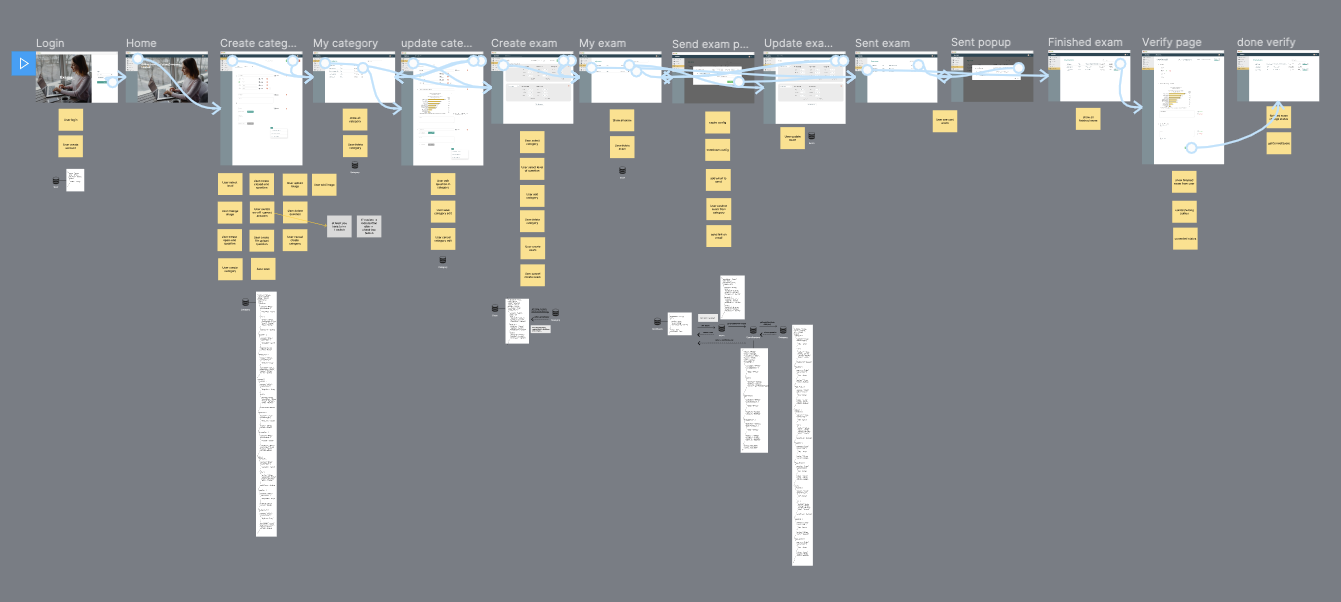
\includegraphics[width=0.9\columnwidth]{exama.png}
  \caption{แสดงตัวอย่างการใช้งาน Figma}
  \label{Fig:useFigma}
\end{figure}

\subsection{สร้างคอนเทนเนอร์}

ทั้งในส่วนต่อประสานกับผู้ใช้(front-end) และส่วนที่จัดการกับฐานข้อมูล(back-end) แต่ละส่วนจะถูกทำให้เป็นคอนเทนเนอร์โดยใช้ Docker เพื่อให้สะดวกต่อการ Deploy ด้วย Kubernetes โดยแต่ละส่วนจะมี Dockerfile ไว้สำหรับสร้างคอนเทนเนอร์อิมเมจของส่วนนั้นๆ โดยเราจะสร้างด้วยวิธี multi-stage build docker ที่จะมาช่วยในการลดขนาดของอิมเมจ ด้วยการนำของจากอิมเมจหนึ่งมาใส่ในอีกอิมเมจหนึ่ง เช่นดังรูป 3.4 

\begin{figure}[H]
  \centering
  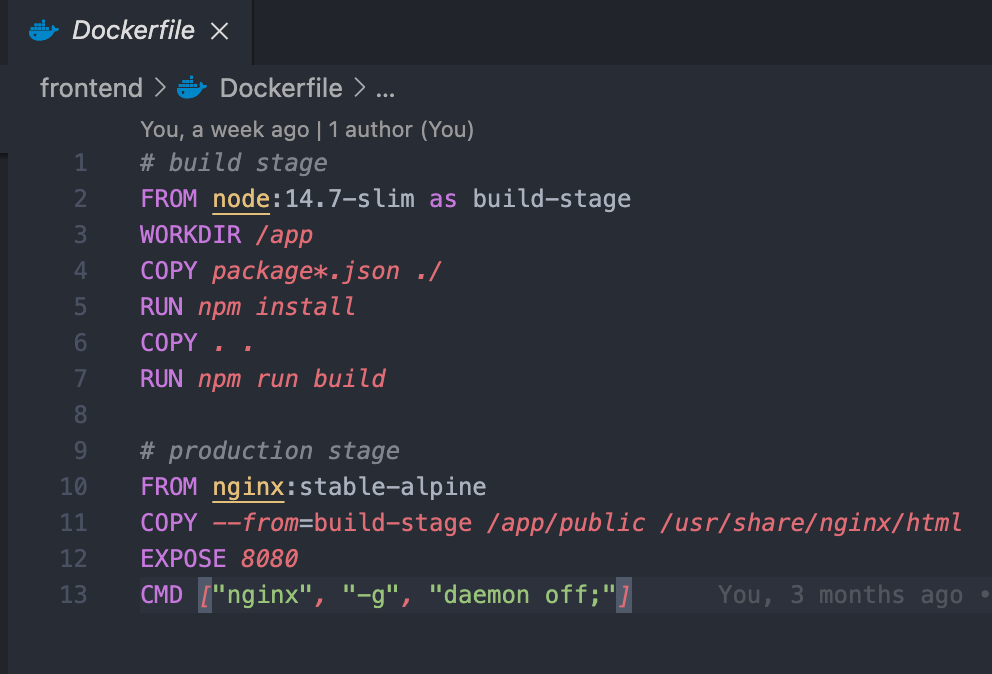
\includegraphics[width=0.9\columnwidth]{dokcerfile.png}
  \caption{แสดงการเขียน Dockerfile ด้วยการทำ multi-stage build docker}
  \label{Fig:useDockerFile}
\end{figure}